\documentclass[twoside]{book}

% Packages required by doxygen
\usepackage{calc}
\usepackage{doxygen}
\usepackage{graphicx}
\usepackage[utf8]{inputenc}
\usepackage{makeidx}
\usepackage{multicol}
\usepackage{multirow}
\usepackage{textcomp}
\usepackage[table]{xcolor}

% Font selection
\usepackage[T1]{fontenc}
\usepackage{mathptmx}
\usepackage[scaled=.90]{helvet}
\usepackage{courier}
\usepackage{amssymb}
\usepackage{sectsty}
\renewcommand{\familydefault}{\sfdefault}
\allsectionsfont{%
  \fontseries{bc}\selectfont%
  \color{darkgray}%
}
\renewcommand{\DoxyLabelFont}{%
  \fontseries{bc}\selectfont%
  \color{darkgray}%
}

% Page & text layout
\usepackage{geometry}
\geometry{%
  a4paper,%
  top=2.5cm,%
  bottom=2.5cm,%
  left=2.5cm,%
  right=2.5cm%
}
\tolerance=750
\hfuzz=15pt
\hbadness=750
\setlength{\emergencystretch}{15pt}
\setlength{\parindent}{0cm}
\setlength{\parskip}{0.2cm}
\makeatletter
\renewcommand{\paragraph}{%
  \@startsection{paragraph}{4}{0ex}{-1.0ex}{1.0ex}{%
    \normalfont\normalsize\bfseries\SS@parafont%
  }%
}
\renewcommand{\subparagraph}{%
  \@startsection{subparagraph}{5}{0ex}{-1.0ex}{1.0ex}{%
    \normalfont\normalsize\bfseries\SS@subparafont%
  }%
}
\makeatother

% Headers & footers
\usepackage{fancyhdr}
\pagestyle{fancyplain}
\fancyhead[LE]{\fancyplain{}{\bfseries\thepage}}
\fancyhead[CE]{\fancyplain{}{}}
\fancyhead[RE]{\fancyplain{}{\bfseries\leftmark}}
\fancyhead[LO]{\fancyplain{}{\bfseries\rightmark}}
\fancyhead[CO]{\fancyplain{}{}}
\fancyhead[RO]{\fancyplain{}{\bfseries\thepage}}
\fancyfoot[LE]{\fancyplain{}{}}
\fancyfoot[CE]{\fancyplain{}{}}
\fancyfoot[RE]{\fancyplain{}{\bfseries\scriptsize Generated on Tue Mar 18 2014 10:36:49 for NATriuM by Doxygen }}
\fancyfoot[LO]{\fancyplain{}{\bfseries\scriptsize Generated on Tue Mar 18 2014 10:36:49 for NATriuM by Doxygen }}
\fancyfoot[CO]{\fancyplain{}{}}
\fancyfoot[RO]{\fancyplain{}{}}
\renewcommand{\footrulewidth}{0.4pt}
\renewcommand{\chaptermark}[1]{%
  \markboth{#1}{}%
}
\renewcommand{\sectionmark}[1]{%
  \markright{\thesection\ #1}%
}

% Indices & bibliography
\usepackage{natbib}
\usepackage[titles]{tocloft}
\setcounter{tocdepth}{3}
\setcounter{secnumdepth}{5}
\makeindex

% Hyperlinks (required, but should be loaded last)
\usepackage{ifpdf}
\ifpdf
  \usepackage[pdftex,pagebackref=true]{hyperref}
\else
  \usepackage[ps2pdf,pagebackref=true]{hyperref}
\fi
\hypersetup{%
  colorlinks=true,%
  linkcolor=blue,%
  citecolor=blue,%
  unicode%
}

% Custom commands
\newcommand{\clearemptydoublepage}{%
  \newpage{\pagestyle{empty}\cleardoublepage}%
}


%===== C O N T E N T S =====

\begin{document}

% Titlepage & ToC
\hypersetup{pageanchor=false}
\pagenumbering{roman}
\begin{titlepage}
\vspace*{7cm}
\begin{center}%
{\Large N\-A\-Triu\-M }\\
\vspace*{1cm}
{\large Generated by Doxygen 1.8.4}\\
\vspace*{0.5cm}
{\small Tue Mar 18 2014 10:36:49}\\
\end{center}
\end{titlepage}
\clearemptydoublepage
\tableofcontents
\clearemptydoublepage
\pagenumbering{arabic}
\hypersetup{pageanchor=true}

%--- Begin generated contents ---
\chapter{Namespace Index}
\section{Namespace List}
Here is a list of all documented namespaces with brief descriptions:\begin{DoxyCompactList}
\item\contentsline{section}{\hyperlink{namespacenatrium_1_1DealIIExtensions}{natrium::DealIIExtensions} (Some extensions to deal.ii )}{\pageref{namespacenatrium_1_1DealIIExtensions}}{}
\item\contentsline{section}{\hyperlink{namespacenatrium_1_1Math}{natrium::Math} (Namespace which contains basic math functions )}{\pageref{namespacenatrium_1_1Math}}{}
\end{DoxyCompactList}

\chapter{Hierarchical Index}
\section{Class Hierarchy}
This inheritance list is sorted roughly, but not completely, alphabetically:\begin{DoxyCompactList}
\item \contentsline{section}{natrium::AdvectionOperator$<$ dim $>$}{\pageref{classnatrium_1_1AdvectionOperator}}{}
\begin{DoxyCompactList}
\item \contentsline{section}{natrium::SEDGMinLee$<$ dim $>$}{\pageref{classnatrium_1_1SEDGMinLee}}{}
\item \contentsline{section}{natrium::SemiLagrangian$<$ dim $>$}{\pageref{classnatrium_1_1SemiLagrangian}}{}
\end{DoxyCompactList}
\item \contentsline{section}{natrium::AdvectionBenchmark::AdvectionResult}{\pageref{structnatrium_1_1AdvectionBenchmark_1_1AdvectionResult}}{}
\item \contentsline{section}{natrium::TaylorGreenVortex2D::AnalyticDensity}{\pageref{classnatrium_1_1TaylorGreenVortex2D_1_1AnalyticDensity}}{}
\item \contentsline{section}{natrium::CouetteFlow2D::AnalyticVelocity}{\pageref{classnatrium_1_1CouetteFlow2D_1_1AnalyticVelocity}}{}
\item \contentsline{section}{natrium::CouetteFlow3D::AnalyticVelocity}{\pageref{classnatrium_1_1CouetteFlow3D_1_1AnalyticVelocity}}{}
\item \contentsline{section}{natrium::PoiseuilleFlow2D::AnalyticVelocity}{\pageref{classnatrium_1_1PoiseuilleFlow2D_1_1AnalyticVelocity}}{}
\item \contentsline{section}{natrium::PoiseuilleFlow3D::AnalyticVelocity}{\pageref{classnatrium_1_1PoiseuilleFlow3D_1_1AnalyticVelocity}}{}
\item \contentsline{section}{natrium::TaylorGreenVortex2D::AnalyticVelocity}{\pageref{classnatrium_1_1TaylorGreenVortex2D_1_1AnalyticVelocity}}{}
\item \contentsline{section}{natrium::Boundary$<$ dim $>$}{\pageref{classnatrium_1_1Boundary}}{}
\item \contentsline{section}{natrium::natrium::Boundary$<$ dim $>$}{\pageref{classnatrium_1_1natrium_1_1Boundary}}{}
\begin{DoxyCompactList}
\item \contentsline{section}{natrium::DoFBoundary$<$ dim $>$}{\pageref{classnatrium_1_1DoFBoundary}}{}
\begin{DoxyCompactList}
\item \contentsline{section}{natrium::GradsBoundary$<$ dim $>$}{\pageref{classnatrium_1_1GradsBoundary}}{}
\end{DoxyCompactList}
\item \contentsline{section}{natrium::LinearFluxBoundary$<$ dim $>$}{\pageref{classnatrium_1_1LinearFluxBoundary}}{}
\begin{DoxyCompactList}
\item \contentsline{section}{natrium::LinearFluxBoundaryRhoU$<$ dim $>$}{\pageref{classnatrium_1_1LinearFluxBoundaryRhoU}}{}
\end{DoxyCompactList}
\item \contentsline{section}{natrium::PeriodicBoundary$<$ dim $>$}{\pageref{classnatrium_1_1PeriodicBoundary}}{}
\end{DoxyCompactList}
\item \contentsline{section}{natrium::BoundaryCollection$<$ dim $>$}{\pageref{classnatrium_1_1BoundaryCollection}}{}
\item \contentsline{section}{natrium::BoundaryTools::BoundaryDensity$<$ dim $>$}{\pageref{classnatrium_1_1BoundaryTools_1_1BoundaryDensity}}{}
\item \contentsline{section}{natrium::BoundaryTestDensity}{\pageref{classnatrium_1_1BoundaryTestDensity}}{}
\item \contentsline{section}{natrium::BoundaryTestVelocity}{\pageref{classnatrium_1_1BoundaryTestVelocity}}{}
\item \contentsline{section}{natrium::BoundaryTools::BoundaryVelocity$<$ dim $>$}{\pageref{classnatrium_1_1BoundaryTools_1_1BoundaryVelocity}}{}
\item \contentsline{section}{natrium::CFDSolver$<$ dim $>$}{\pageref{classnatrium_1_1CFDSolver}}{}
\begin{DoxyCompactList}
\item \contentsline{section}{natrium::BenchmarkCFDSolver$<$ dim $>$}{\pageref{classnatrium_1_1BenchmarkCFDSolver}}{}
\end{DoxyCompactList}
\item \contentsline{section}{natrium::Checkpoint$<$ dim $>$}{\pageref{classnatrium_1_1Checkpoint}}{}
\item \contentsline{section}{natrium::CheckpointStatus}{\pageref{structnatrium_1_1CheckpointStatus}}{}
\item \contentsline{section}{natrium::CollisionModel}{\pageref{classnatrium_1_1CollisionModel}}{}
\begin{DoxyCompactList}
\item \contentsline{section}{natrium::BGK}{\pageref{classnatrium_1_1BGK}}{}
\begin{DoxyCompactList}
\item \contentsline{section}{natrium::BGKIncompressible}{\pageref{classnatrium_1_1BGKIncompressible}}{}
\item \contentsline{section}{natrium::BGKMultistep}{\pageref{classnatrium_1_1BGKMultistep}}{}
\item \contentsline{section}{natrium::BGKPseudopotential$<$ dim $>$}{\pageref{classnatrium_1_1BGKPseudopotential}}{}
\item \contentsline{section}{natrium::BGKStandard}{\pageref{classnatrium_1_1BGKStandard}}{}
\item \contentsline{section}{natrium::BGKStandardTransformed}{\pageref{classnatrium_1_1BGKStandardTransformed}}{}
\item \contentsline{section}{natrium::BGKSteadyState}{\pageref{classnatrium_1_1BGKSteadyState}}{}
\end{DoxyCompactList}
\item \contentsline{section}{natrium::MRT}{\pageref{classnatrium_1_1MRT}}{}
\begin{DoxyCompactList}
\item \contentsline{section}{natrium::KBCCentral}{\pageref{classnatrium_1_1KBCCentral}}{}
\item \contentsline{section}{natrium::KBCStandard}{\pageref{classnatrium_1_1KBCStandard}}{}
\item \contentsline{section}{natrium::MRTStandard}{\pageref{classnatrium_1_1MRTStandard}}{}
\end{DoxyCompactList}
\end{DoxyCompactList}
\item \contentsline{section}{natrium::ConstantExternalForce$<$ dim $>$}{\pageref{classnatrium_1_1ConstantExternalForce}}{}
\item \contentsline{section}{natrium::DataProcessor$<$ dim $>$}{\pageref{classnatrium_1_1DataProcessor}}{}
\begin{DoxyCompactList}
\item \contentsline{section}{natrium::GlobalTurbulenceStats$<$ dim $>$}{\pageref{classnatrium_1_1GlobalTurbulenceStats}}{}
\end{DoxyCompactList}
\item \contentsline{section}{natrium::DataProcessor$<$ 2 $>$}{\pageref{classnatrium_1_1DataProcessor}}{}
\begin{DoxyCompactList}
\item \contentsline{section}{EnstrophySubdomain}{\pageref{classEnstrophySubdomain}}{}
\item \contentsline{section}{natrium::CompareToBotella}{\pageref{classnatrium_1_1CompareToBotella}}{}
\item \contentsline{section}{natrium::CompareToErturk}{\pageref{classnatrium_1_1CompareToErturk}}{}
\item \contentsline{section}{natrium::CompareToGhia}{\pageref{classnatrium_1_1CompareToGhia}}{}
\end{DoxyCompactList}
\item \contentsline{section}{natrium::DataProcessor$<$ 3 $>$}{\pageref{classnatrium_1_1DataProcessor}}{}
\begin{DoxyCompactList}
\item \contentsline{section}{natrium::FinalChannelStatistics}{\pageref{classnatrium_1_1FinalChannelStatistics}}{}
\end{DoxyCompactList}
\item \contentsline{section}{natrium::DistributionFunctions}{\pageref{classnatrium_1_1DistributionFunctions}}{}
\item \contentsline{section}{natrium::ErrorStats$<$ dim $>$}{\pageref{classnatrium_1_1ErrorStats}}{}
\item \contentsline{section}{natrium::FFTW2D}{\pageref{classnatrium_1_1FFTW2D}}{}
\item \contentsline{section}{natrium::Filter$<$ dim $>$}{\pageref{classnatrium_1_1Filter}}{}
\begin{DoxyCompactList}
\item \contentsline{section}{natrium::ExponentialFilter$<$ dim $>$}{\pageref{classnatrium_1_1ExponentialFilter}}{}
\item \contentsline{section}{natrium::NewFilter$<$ dim $>$}{\pageref{classnatrium_1_1NewFilter}}{}
\end{DoxyCompactList}
\item \contentsline{section}{HtmlTrace}{\pageref{classHtmlTrace}}{}
\item \contentsline{section}{natrium::TurbulentChannelFlow3D::IncompressibleU}{\pageref{classnatrium_1_1TurbulentChannelFlow3D_1_1IncompressibleU}}{}
\item \contentsline{section}{natrium::BackwardFacingStep2D::InflowVelocity}{\pageref{classnatrium_1_1BackwardFacingStep2D_1_1InflowVelocity}}{}
\item \contentsline{section}{natrium::DiamondObstacle2D::InflowVelocity}{\pageref{classnatrium_1_1DiamondObstacle2D_1_1InflowVelocity}}{}
\item \contentsline{section}{natrium::Hill3D::InflowVelocity}{\pageref{classnatrium_1_1Hill3D_1_1InflowVelocity}}{}
\item \contentsline{section}{natrium::TaylorGreenVortex3D::InitialDensity}{\pageref{classnatrium_1_1TaylorGreenVortex3D_1_1InitialDensity}}{}
\item \contentsline{section}{natrium::Droplet2D::InitialDensity}{\pageref{classnatrium_1_1Droplet2D_1_1InitialDensity}}{}
\item \contentsline{section}{natrium::TaylorGreenVortex3D::InitialVelocity}{\pageref{classnatrium_1_1TaylorGreenVortex3D_1_1InitialVelocity}}{}
\item \contentsline{section}{natrium::DecayingTurbulence2D::InitialVelocity}{\pageref{classnatrium_1_1DecayingTurbulence2D_1_1InitialVelocity}}{}
\item \contentsline{section}{natrium::SteadyPeriodicTestFlow2D::InitialVelocity}{\pageref{classnatrium_1_1SteadyPeriodicTestFlow2D_1_1InitialVelocity}}{}
\item \contentsline{section}{natrium::BackwardFacingStep2D::InitialVelocity}{\pageref{classnatrium_1_1BackwardFacingStep2D_1_1InitialVelocity}}{}
\item \contentsline{section}{natrium::TurbulentChannelFlow3D::InitialVelocity}{\pageref{classnatrium_1_1TurbulentChannelFlow3D_1_1InitialVelocity}}{}
\item \contentsline{section}{natrium::Droplet2D::InitialVelocity}{\pageref{classnatrium_1_1Droplet2D_1_1InitialVelocity}}{}
\item \contentsline{section}{natrium::LubricationSine::InitialVelocity}{\pageref{classnatrium_1_1LubricationSine_1_1InitialVelocity}}{}
\item \contentsline{section}{natrium::ShearLayer2D::InitialVelocity}{\pageref{classnatrium_1_1ShearLayer2D_1_1InitialVelocity}}{}
\item \contentsline{section}{natrium::SinusoidalShear2D::InitialVelocity}{\pageref{classnatrium_1_1SinusoidalShear2D_1_1InitialVelocity}}{}
\item \contentsline{section}{natrium::InitMPI}{\pageref{structnatrium_1_1InitMPI}}{}
\item \contentsline{section}{natrium::SemiLagrangian$<$ dim $>$::LagrangianPathDestination}{\pageref{structnatrium_1_1SemiLagrangian_1_1LagrangianPathDestination}}{}
\item \contentsline{section}{natrium::SemiLagrangian$<$ dim $>$::LagrangianPathTracker}{\pageref{structnatrium_1_1SemiLagrangian_1_1LagrangianPathTracker}}{}
\item \contentsline{section}{natrium::Logging}{\pageref{classnatrium_1_1Logging}}{}
\item \contentsline{section}{natrium::matrixAnalysis$<$ dim $>$}{\pageref{classnatrium_1_1matrixAnalysis}}{}
\item \contentsline{section}{natrium::TurbulentChannelFlow3D::MeanVelocityProfile}{\pageref{classnatrium_1_1TurbulentChannelFlow3D_1_1MeanVelocityProfile}}{}
\item \contentsline{section}{plb::ModIncomprFlowParam$<$ T $>$}{\pageref{classplb_1_1ModIncomprFlowParam}}{}
\item \contentsline{section}{natrium::MPIGuard}{\pageref{classnatrium_1_1MPIGuard}}{}
\item \contentsline{section}{natrium::MultistepCollisionData}{\pageref{classnatrium_1_1MultistepCollisionData}}{}
\begin{DoxyCompactList}
\item \contentsline{section}{natrium::BGKMultistep}{\pageref{classnatrium_1_1BGKMultistep}}{}
\end{DoxyCompactList}
\item \contentsline{section}{natrium::NATriuMException}{\pageref{classnatrium_1_1NATriuMException}}{}
\begin{DoxyCompactList}
\item \contentsline{section}{natrium::AdvectionSolverException}{\pageref{classnatrium_1_1AdvectionSolverException}}{}
\item \contentsline{section}{natrium::BoundaryCollectionException}{\pageref{classnatrium_1_1BoundaryCollectionException}}{}
\item \contentsline{section}{natrium::BoundaryTools::BoundaryException}{\pageref{classnatrium_1_1BoundaryTools_1_1BoundaryException}}{}
\item \contentsline{section}{natrium::CFDSolverException}{\pageref{classnatrium_1_1CFDSolverException}}{}
\item \contentsline{section}{natrium::CFDSolverUtilities::CFDSolverUtilitiesException}{\pageref{classnatrium_1_1CFDSolverUtilities_1_1CFDSolverUtilitiesException}}{}
\item \contentsline{section}{natrium::CheckpointException}{\pageref{classnatrium_1_1CheckpointException}}{}
\item \contentsline{section}{natrium::CollisionException}{\pageref{classnatrium_1_1CollisionException}}{}
\item \contentsline{section}{natrium::ConfigurationException}{\pageref{classnatrium_1_1ConfigurationException}}{}
\item \contentsline{section}{natrium::PeriodicBoundaryNotPossible}{\pageref{classnatrium_1_1PeriodicBoundaryNotPossible}}{}
\item \contentsline{section}{natrium::SemiLagrangianException}{\pageref{classnatrium_1_1SemiLagrangianException}}{}
\end{DoxyCompactList}
\item \contentsline{section}{natrium::own\_\-double\_\-less}{\pageref{classnatrium_1_1own__double__less}}{}
\item \contentsline{section}{natrium::PhysicalProperties$<$ dim $>$}{\pageref{classnatrium_1_1PhysicalProperties}}{}
\item \contentsline{section}{natrium::BoundaryTools::point\_\-sorter}{\pageref{classnatrium_1_1BoundaryTools_1_1point__sorter}}{}
\item \contentsline{section}{natrium::ProblemDescription$<$ dim $>$}{\pageref{classnatrium_1_1ProblemDescription}}{}
\begin{DoxyCompactList}
\item \contentsline{section}{natrium::Benchmark$<$ 2 $>$}{\pageref{classnatrium_1_1Benchmark}}{}
\begin{DoxyCompactList}
\item \contentsline{section}{natrium::CouetteFlow2D}{\pageref{classnatrium_1_1CouetteFlow2D}}{}
\item \contentsline{section}{natrium::PoiseuilleFlow2D}{\pageref{classnatrium_1_1PoiseuilleFlow2D}}{}
\item \contentsline{section}{natrium::TaylorGreenVortex2D}{\pageref{classnatrium_1_1TaylorGreenVortex2D}}{}
\end{DoxyCompactList}
\item \contentsline{section}{natrium::Benchmark$<$ 3 $>$}{\pageref{classnatrium_1_1Benchmark}}{}
\begin{DoxyCompactList}
\item \contentsline{section}{natrium::CouetteFlow3D}{\pageref{classnatrium_1_1CouetteFlow3D}}{}
\item \contentsline{section}{natrium::PoiseuilleFlow3D}{\pageref{classnatrium_1_1PoiseuilleFlow3D}}{}
\end{DoxyCompactList}
\item \contentsline{section}{natrium::Benchmark$<$ dim $>$}{\pageref{classnatrium_1_1Benchmark}}{}
\end{DoxyCompactList}
\item \contentsline{section}{natrium::ProblemDescription$<$ 2 $>$}{\pageref{classnatrium_1_1ProblemDescription}}{}
\begin{DoxyCompactList}
\item \contentsline{section}{natrium::BackwardFacingStep2D}{\pageref{classnatrium_1_1BackwardFacingStep2D}}{}
\item \contentsline{section}{natrium::ComplexWall1}{\pageref{classnatrium_1_1ComplexWall1}}{}
\item \contentsline{section}{natrium::Cylinder2D}{\pageref{classnatrium_1_1Cylinder2D}}{}
\item \contentsline{section}{natrium::DecayingTurbulence2D}{\pageref{classnatrium_1_1DecayingTurbulence2D}}{}
\item \contentsline{section}{natrium::DensityFluctuation2D}{\pageref{classnatrium_1_1DensityFluctuation2D}}{}
\item \contentsline{section}{natrium::DiamondObstacle2D}{\pageref{classnatrium_1_1DiamondObstacle2D}}{}
\item \contentsline{section}{natrium::Droplet2D}{\pageref{classnatrium_1_1Droplet2D}}{}
\item \contentsline{section}{natrium::LidDrivenCavity2D}{\pageref{classnatrium_1_1LidDrivenCavity2D}}{}
\item \contentsline{section}{natrium::LubricationSine}{\pageref{classnatrium_1_1LubricationSine}}{}
\item \contentsline{section}{natrium::PeriodicTestDomain2D}{\pageref{classnatrium_1_1PeriodicTestDomain2D}}{}
\item \contentsline{section}{natrium::ShearLayer2D}{\pageref{classnatrium_1_1ShearLayer2D}}{}
\item \contentsline{section}{natrium::SinusoidalShear2D}{\pageref{classnatrium_1_1SinusoidalShear2D}}{}
\item \contentsline{section}{natrium::SteadyPeriodicTestFlow2D}{\pageref{classnatrium_1_1SteadyPeriodicTestFlow2D}}{}
\begin{DoxyCompactList}
\item \contentsline{section}{natrium::UnsteadyPeriodicTestFlow2D}{\pageref{classnatrium_1_1UnsteadyPeriodicTestFlow2D}}{}
\end{DoxyCompactList}
\item \contentsline{section}{TaylorGreenTest2D}{\pageref{classTaylorGreenTest2D}}{}
\item \contentsline{section}{WallTestDomain2D}{\pageref{classWallTestDomain2D}}{}
\end{DoxyCompactList}
\item \contentsline{section}{natrium::ProblemDescription$<$ 3 $>$}{\pageref{classnatrium_1_1ProblemDescription}}{}
\begin{DoxyCompactList}
\item \contentsline{section}{natrium::Hill3D}{\pageref{classnatrium_1_1Hill3D}}{}
\item \contentsline{section}{natrium::PeriodicTestDomain3D}{\pageref{classnatrium_1_1PeriodicTestDomain3D}}{}
\item \contentsline{section}{natrium::TaylorGreenVortex3D}{\pageref{classnatrium_1_1TaylorGreenVortex3D}}{}
\item \contentsline{section}{natrium::TurbulentChannelFlow3D}{\pageref{classnatrium_1_1TurbulentChannelFlow3D}}{}
\end{DoxyCompactList}
\item \contentsline{section}{natrium::PseudopotentialParameters}{\pageref{structnatrium_1_1PseudopotentialParameters}}{}
\item \contentsline{section}{natrium::SemiParallelMatrix$<$ VECTOR $>$}{\pageref{classnatrium_1_1SemiParallelMatrix}}{}
\item \contentsline{section}{SinusShapeDomain2D$<$ T $>$}{\pageref{classSinusShapeDomain2D}}{}
\item \contentsline{section}{natrium::SolverConfiguration}{\pageref{classnatrium_1_1SolverConfiguration}}{}
\item \contentsline{section}{natrium::SolverStats$<$ dim $>$}{\pageref{classnatrium_1_1SolverStats}}{}
\item \contentsline{section}{natrium::KBCCentral::stabilizer}{\pageref{structnatrium_1_1KBCCentral_1_1stabilizer}}{}
\item \contentsline{section}{natrium::KBCStandard::stabilizer}{\pageref{structnatrium_1_1KBCStandard_1_1stabilizer}}{}
\item \contentsline{section}{natrium::StatsInPlane$<$ dim $>$}{\pageref{classnatrium_1_1StatsInPlane}}{}
\item \contentsline{section}{natrium::Stencil}{\pageref{classnatrium_1_1Stencil}}{}
\begin{DoxyCompactList}
\item \contentsline{section}{natrium::D2Q9}{\pageref{classnatrium_1_1D2Q9}}{}
\item \contentsline{section}{natrium::D3Q15}{\pageref{classnatrium_1_1D3Q15}}{}
\item \contentsline{section}{natrium::D3Q19}{\pageref{classnatrium_1_1D3Q19}}{}
\item \contentsline{section}{natrium::D3Q27}{\pageref{classnatrium_1_1D3Q27}}{}
\end{DoxyCompactList}
\item \contentsline{section}{natrium::IntegrationTestCases::TestResult}{\pageref{structnatrium_1_1IntegrationTestCases_1_1TestResult}}{}
\item \contentsline{section}{natrium::TimeIntegrator$<$ MATRIX, VECTOR $>$}{\pageref{classnatrium_1_1TimeIntegrator}}{}
\begin{DoxyCompactList}
\item \contentsline{section}{natrium::DealIIWrapper$<$ MATRIX, VECTOR $>$}{\pageref{classnatrium_1_1DealIIWrapper}}{}
\item \contentsline{section}{natrium::ExponentialTimeIntegrator$<$ MATRIX, VECTOR $>$}{\pageref{classnatrium_1_1ExponentialTimeIntegrator}}{}
\item \contentsline{section}{natrium::RungeKutta5LowStorage$<$ MATRIX, VECTOR $>$}{\pageref{classnatrium_1_1RungeKutta5LowStorage}}{}
\item \contentsline{section}{natrium::ThetaMethod$<$ MATRIX, VECTOR $>$}{\pageref{classnatrium_1_1ThetaMethod}}{}
\end{DoxyCompactList}
\item \contentsline{section}{natrium::Timing}{\pageref{classnatrium_1_1Timing}}{}
\item \contentsline{section}{natrium::TurbulenceStats$<$ dim $>$}{\pageref{classnatrium_1_1TurbulenceStats}}{}
\item \contentsline{section}{natrium::UnsteadyPeriodicTestFlow2D::UnsteadyInitialVelocity}{\pageref{classnatrium_1_1UnsteadyPeriodicTestFlow2D_1_1UnsteadyInitialVelocity}}{}
\item \contentsline{section}{natrium::TurbulentChannelFlow3D::UnstructuredGridFunc}{\pageref{structnatrium_1_1TurbulentChannelFlow3D_1_1UnstructuredGridFunc}}{}
\item \contentsline{section}{natrium::VmultLimiter}{\pageref{classnatrium_1_1VmultLimiter}}{}
\end{DoxyCompactList}

\chapter{Class Index}
\section{Class List}
Here are the classes, structs, unions and interfaces with brief descriptions\-:\begin{DoxyCompactList}
\item\contentsline{section}{\hyperlink{classnatrium_1_1AdvectionOperator}{natrium\-::\-Advection\-Operator$<$ dim $>$} \\*Abstract class for spatial part of the Advection Operator e\-\_\-i $\ast$ dx\-\_\-i f }{\pageref{classnatrium_1_1AdvectionOperator}}{}
\item\contentsline{section}{\hyperlink{classnatrium_1_1AdvectionSolverException}{natrium\-::\-Advection\-Solver\-Exception} \\*Exception class for Advection\-Solver }{\pageref{classnatrium_1_1AdvectionSolverException}}{}
\item\contentsline{section}{\hyperlink{classnatrium_1_1BGKTransformed}{natrium\-::\-B\-G\-K\-Transformed} \\*Description of the B\-G\-K model for the transformed particle distributions, as described in Global data which is used by Min and Lee (2011)\-: A spectral-\/element discontinuous Galerkin lattice Boltzmann method for nearly incompressible flows, J\-C\-P 230 pp. 245-\/259 }{\pageref{classnatrium_1_1BGKTransformed}}{}
\item\contentsline{section}{\hyperlink{classnatrium_1_1BoltzmannModel}{natrium\-::\-Boltzmann\-Model} \\*Abstract class for the description of a boltzmann model, e.\-g. D2\-Q9 }{\pageref{classnatrium_1_1BoltzmannModel}}{}
\item\contentsline{section}{\hyperlink{classnatrium_1_1Boundary}{natrium\-::\-Boundary$<$ dim $>$} \\*Abstract class for the description of boundaries. Base class of \hyperlink{classnatrium_1_1PeriodicBoundary}{Periodic\-Boundary}, Inflow\-Boundary, etc }{\pageref{classnatrium_1_1Boundary}}{}
\item\contentsline{section}{\hyperlink{classnatrium_1_1BoundaryCollection}{natrium\-::\-Boundary\-Collection$<$ dim $>$} }{\pageref{classnatrium_1_1BoundaryCollection}}{}
\item\contentsline{section}{\hyperlink{classnatrium_1_1CFDSolver}{natrium\-::\-C\-F\-D\-Solver$<$ dim $>$} \\*The central class for the C\-F\-D simulation based on the D\-B\-E }{\pageref{classnatrium_1_1CFDSolver}}{}
\item\contentsline{section}{\hyperlink{classnatrium_1_1CFDSolverException}{natrium\-::\-C\-F\-D\-Solver\-Exception} \\*Exception class for \hyperlink{classnatrium_1_1CFDSolver}{C\-F\-D\-Solver} }{\pageref{classnatrium_1_1CFDSolverException}}{}
\item\contentsline{section}{\hyperlink{classnatrium_1_1CollisionModel}{natrium\-::\-Collision\-Model} \\*Abstract class for the description of collision schemes }{\pageref{classnatrium_1_1CollisionModel}}{}
\item\contentsline{section}{\hyperlink{classnatrium_1_1ConfigurationException}{natrium\-::\-Configuration\-Exception} \\*Exception class for \hyperlink{classnatrium_1_1CFDSolver}{C\-F\-D\-Solver} }{\pageref{classnatrium_1_1ConfigurationException}}{}
\item\contentsline{section}{\hyperlink{classnatrium_1_1CouetteFlow2D}{natrium\-::\-Couette\-Flow2\-D} \\*Description of a simple Couette Flow (regular channel flow in square domain). The domain is \mbox{[}0,1\mbox{]}$^\wedge$2. The top plate is moved with constant velocity. The domain consists of 8 x 8 = 64 Elements (contrast to Min and Lee, who have 6 x 6) }{\pageref{classnatrium_1_1CouetteFlow2D}}{}
\item\contentsline{section}{\hyperlink{classnatrium_1_1D2Q9IncompressibleModel}{natrium\-::\-D2\-Q9\-Incompressible\-Model} \\*D2\-Q9 model description for incompressible flow }{\pageref{classnatrium_1_1D2Q9IncompressibleModel}}{}
\item\contentsline{section}{\hyperlink{classnatrium_1_1D2Q9Model}{natrium\-::\-D2\-Q9\-Model} \\*D2\-Q9 Model }{\pageref{classnatrium_1_1D2Q9Model}}{}
\item\contentsline{section}{\hyperlink{classnatrium_1_1ExponentialTimeIntegrator}{natrium\-::\-Exponential\-Time\-Integrator} \\*Exponential time integration scheme for the solution of f' = L$\ast$f, as used in Uga etal. (2012) Spectral-\/element discontinuous Galerkin lattice Boltzmann simulation of flow past two cylinders in tandem with an exponential time integrator, C\-M\-W\-A 65 pp. 239-\/251 }{\pageref{classnatrium_1_1ExponentialTimeIntegrator}}{}
\item\contentsline{section}{\hyperlink{classnatrium_1_1Logging}{natrium\-::\-Logging} \\*This class is responsible for output streams to the command line and log file }{\pageref{classnatrium_1_1Logging}}{}
\item\contentsline{section}{\hyperlink{classnatrium_1_1own__double__less}{natrium\-::own\-\_\-double\-\_\-less} \\*Function to compare doubles as map keys; regards two doubles equal if they are in a epsilon(=1e-\/7)-\/range }{\pageref{classnatrium_1_1own__double__less}}{}
\item\contentsline{section}{\hyperlink{classnatrium_1_1PeriodicBoundary}{natrium\-::\-Periodic\-Boundary$<$ dim $>$} \\*A periodic boundary condition, }{\pageref{classnatrium_1_1PeriodicBoundary}}{}
\item\contentsline{section}{\hyperlink{classnatrium_1_1PeriodicBoundaryNotPossible}{natrium\-::\-Periodic\-Boundary\-Not\-Possible} \\*Exception for impossible periodic boundary, e.\-g. when the interfaces don't have the same length }{\pageref{classnatrium_1_1PeriodicBoundaryNotPossible}}{}
\item\contentsline{section}{\hyperlink{classnatrium_1_1PeriodicTestDomain2D}{natrium\-::\-Periodic\-Test\-Domain2\-D} \\*Description of a simple Periodic Flow (flow in square domain). The domain is \mbox{[}0,1\mbox{]}$^\wedge$2. The domain consists of 4 elements }{\pageref{classnatrium_1_1PeriodicTestDomain2D}}{}
\item\contentsline{section}{\hyperlink{classnatrium_1_1PoiseuilleFlow2D}{natrium\-::\-Poiseuille\-Flow2\-D} \\*Description of a simple Channel Flow The domain is \mbox{[}0,5\mbox{]}x\mbox{[}0,1\mbox{]} }{\pageref{classnatrium_1_1PoiseuilleFlow2D}}{}
\item\contentsline{section}{\hyperlink{classnatrium_1_1ProblemDescription}{natrium\-::\-Problem\-Description$<$ dim $>$} \\*Abstract class for the description of a C\-F\-D problem. The description includes the computational mesh, boundary description, viscosity and initial values }{\pageref{classnatrium_1_1ProblemDescription}}{}
\item\contentsline{section}{\hyperlink{classnatrium_1_1RungeKutta5LowStorage}{natrium\-::\-Runge\-Kutta5\-Low\-Storage} \\*Implementation of the fifth-\/order Runge-\/\-Kutta time integration scheme with low storage consumption }{\pageref{classnatrium_1_1RungeKutta5LowStorage}}{}
\item\contentsline{section}{\hyperlink{classnatrium_1_1SEDGMinLee}{natrium\-::\-S\-E\-D\-G\-Min\-Lee$<$ dim $>$} \\*This class solves the linear advection equations by a scheme which is used, e.\-g., by Min and Lee (2011)\-: A spectral-\/element discontinuous Galerkin lattice Boltzmann method for nearly incompressible flows, J\-C\-P 230 pp. 245-\/259. The advection equations used in the Lattice Boltzmann on unstructured grids are \[ \partial_t f_i + e_i \partial_x f_i = 0,\quad \forall i = 1,\dots,Q-1 \] where $ f_i(x,t) $ are the particle distribution functions, and $ e_i $ are the particle velocities. The discontinuous Galerkin (D\-G) method turns these P\-D\-Es into a large system of O\-D\-Es which can then be solved by a time integration scheme. Whereas this class implements the S\-E\-D\-G spatial discretization, the time integration is done by a subclass of \hyperlink{classnatrium_1_1TimeIntegrator}{Time\-Integrator}, e.\-g. \hyperlink{classnatrium_1_1RungeKutta5LowStorage}{Runge\-Kutta5\-Low\-Storage}. In other Finite Element schemes, degrees of freedom can belong to different elements (e.\-g. at corners of elements). In contrast, D\-G methods have the degrees of freedom belonging to a single element, which can lead to discontinuities at the element faces. To connect neighbor cells, the integral over the boundary of each cell incorporates the solution on neighbor cells. These contributions are called numerical fluxes. The D\-G scheme uses the weak formulation of the above equations on quadrilateral elements \$\$\-: \[ \left( \partial_t f_i + \partial_x (e_i f_i), \Phi \right)_{\Omega_e} = \left(n \left[ e_i f_i - F^{\ast}_{i}(f) \right], \Phi \right)_{\partial \Omega_e}. \] In this formulation $ F^{\ast}_{i}(f) $ denotes the numerical fluxes. They can be be calculated as central fluxes or Lax-\/\-Friedrichs fluxes. Lax-\/\-Friedrichs is in general more accurate for the advection equation. For detailed information on the fluxes, see the cited paper. For spatial integration a Gauss-\/\-Lobatto quadrature is used, which has the advantage that the resulting mass matrix M\-\_\-i = (, )\-\_\-\{\} is diagonal. This circumvents the solution of a linear equation system. including particle distributions f, system matrix L, diagonal mass matrix M, gradient matrices Dx, Dy, (Dz) and boundary matrix R }{\pageref{classnatrium_1_1SEDGMinLee}}{}
\item\contentsline{section}{\hyperlink{classnatrium_1_1SolverConfiguration}{natrium\-::\-Solver\-Configuration} \\*Class that stores the configuration for a C\-F\-D simulation based on the Discrete Boltzmann Equation (D\-B\-E) }{\pageref{classnatrium_1_1SolverConfiguration}}{}
\item\contentsline{section}{\hyperlink{classnatrium_1_1SteadyPeriodicTestFlow2D}{natrium\-::\-Steady\-Periodic\-Test\-Flow2\-D} \\*Description of a simple Periodic Flow (flow in square domain). The domain is \mbox{[}0,1\mbox{]}$^\wedge$2. The domain consists of 8 x 8 = 64 Elements (contrast to Min and Lee, who have 6 x 6) }{\pageref{classnatrium_1_1SteadyPeriodicTestFlow2D}}{}
\item\contentsline{section}{\hyperlink{classnatrium_1_1TaylorGreenVortex2D}{natrium\-::\-Taylor\-Green\-Vortex2\-D} \\*Description of a simple Periodic Flow (flow in square domain). The domain is \mbox{[}0,1\mbox{]}$^\wedge$2. The domain consists of 8 x 8 = 64 Elements (contrast to Min and Lee, who have 6 x 6) }{\pageref{classnatrium_1_1TaylorGreenVortex2D}}{}
\item\contentsline{section}{\hyperlink{classnatrium_1_1TimeIntegrator}{natrium\-::\-Time\-Integrator} \\*Abstract class for time integration (solution of ordinary differential equations (O\-D\-E)) }{\pageref{classnatrium_1_1TimeIntegrator}}{}
\item\contentsline{section}{\hyperlink{classnatrium_1_1UnsteadyPeriodicTestFlow2D}{natrium\-::\-Unsteady\-Periodic\-Test\-Flow2\-D} }{\pageref{classnatrium_1_1UnsteadyPeriodicTestFlow2D}}{}
\end{DoxyCompactList}

\chapter{File Index}
\section{\-File \-List}
\-Here is a list of all documented files with brief descriptions\-:\begin{DoxyCompactList}
\item\contentsline{section}{/home/kraemer/eclipse\-\_\-workspace/\-N\-A\-Triu\-M/src/benchmarks/\hyperlink{CouetteFlow2D_8cpp}{\-Couette\-Flow2\-D.\-cpp} }{\pageref{CouetteFlow2D_8cpp}}{}
\item\contentsline{section}{/home/kraemer/eclipse\-\_\-workspace/\-N\-A\-Triu\-M/src/benchmarks/\hyperlink{CouetteFlow2D_8h}{\-Couette\-Flow2\-D.\-h} \\*\-Description of a simple \-Couette \-Flow (regular channel flow in rectangular domain) }{\pageref{CouetteFlow2D_8h}}{}
\item\contentsline{section}{/home/kraemer/eclipse\-\_\-workspace/\-N\-A\-Triu\-M/src/boltzmannmodels/\hyperlink{BoltzmannModel_8cpp}{\-Boltzmann\-Model.\-cpp} \\*\-Abstract class for the description of a boltzmann model }{\pageref{BoltzmannModel_8cpp}}{}
\item\contentsline{section}{/home/kraemer/eclipse\-\_\-workspace/\-N\-A\-Triu\-M/src/boltzmannmodels/\hyperlink{BoltzmannModel_8h}{\-Boltzmann\-Model.\-h} \\*\-Abstract class for the description of a boltzmann model }{\pageref{BoltzmannModel_8h}}{}
\item\contentsline{section}{/home/kraemer/eclipse\-\_\-workspace/\-N\-A\-Triu\-M/src/boltzmannmodels/{\bfseries \-D2\-Q9\-Incompressible\-Model.\-h} }{\pageref{D2Q9IncompressibleModel_8h}}{}
\item\contentsline{section}{/home/kraemer/eclipse\-\_\-workspace/\-N\-A\-Triu\-M/src/boltzmannmodels/\hyperlink{D2Q9Model_8cpp}{\-D2\-Q9\-Model.\-cpp} }{\pageref{D2Q9Model_8cpp}}{}
\item\contentsline{section}{/home/kraemer/eclipse\-\_\-workspace/\-N\-A\-Triu\-M/src/boltzmannmodels/\hyperlink{D2Q9Model_8h}{\-D2\-Q9\-Model.\-h} \\*\-D2\-Q9 \-Boltzmann \-Model }{\pageref{D2Q9Model_8h}}{}
\item\contentsline{section}{/home/kraemer/eclipse\-\_\-workspace/\-N\-A\-Triu\-M/src/collisionmodels/\hyperlink{BGKTransformed_8cpp}{\-B\-G\-K\-Transformed.\-cpp} }{\pageref{BGKTransformed_8cpp}}{}
\item\contentsline{section}{/home/kraemer/eclipse\-\_\-workspace/\-N\-A\-Triu\-M/src/collisionmodels/\hyperlink{BGKTransformed_8h}{\-B\-G\-K\-Transformed.\-h} \\*\-Description of the \-B\-G\-K model for the transformed particle distributions, as described in \-Global data which is used by \-Min and \-Lee (2011)\-: \-A spectral-\/elemennt discontinuous \-Galerkin lattice \-Boltzmann method for nearly incompressible flows, \-J\-C\-P 230 pp. 245-\/259 }{\pageref{BGKTransformed_8h}}{}
\item\contentsline{section}{/home/kraemer/eclipse\-\_\-workspace/\-N\-A\-Triu\-M/src/collisionmodels/\hyperlink{CollisionModel_8cpp}{\-Collision\-Model.\-cpp} }{\pageref{CollisionModel_8cpp}}{}
\item\contentsline{section}{/home/kraemer/eclipse\-\_\-workspace/\-N\-A\-Triu\-M/src/collisionmodels/\hyperlink{CollisionModel_8h}{\-Collision\-Model.\-h} \\*\-Abstract class for the description of collision schemes }{\pageref{CollisionModel_8h}}{}
\item\contentsline{section}{/home/kraemer/eclipse\-\_\-workspace/\-N\-A\-Triu\-M/src/problemdescription/\hyperlink{ProblemDescription_8cpp}{\-Problem\-Description.\-cpp} }{\pageref{ProblemDescription_8cpp}}{}
\item\contentsline{section}{/home/kraemer/eclipse\-\_\-workspace/\-N\-A\-Triu\-M/src/problemdescription/\hyperlink{ProblemDescription_8h}{\-Problem\-Description.\-h} \\*\-Abstract class for the description of a \-C\-F\-D problem. \-The description includes the computational mesh, boundary description, viscosity and initial values }{\pageref{ProblemDescription_8h}}{}
\item\contentsline{section}{/home/kraemer/eclipse\-\_\-workspace/\-N\-A\-Triu\-M/src/problemdescription/\hyperlink{SimpleProblemDescription2D_8cpp}{\-Simple\-Problem\-Description2\-D.\-cpp} }{\pageref{SimpleProblemDescription2D_8cpp}}{}
\item\contentsline{section}{/home/kraemer/eclipse\-\_\-workspace/\-N\-A\-Triu\-M/src/problemdescription/\hyperlink{SimpleProblemDescription2D_8h}{\-Simple\-Problem\-Description2\-D.\-h} \\*\-Description of simple 2\-D test problems, using boundary \-I\-Ds and easy-\/to-\/use boundary functions }{\pageref{SimpleProblemDescription2D_8h}}{}
\item\contentsline{section}{/home/kraemer/eclipse\-\_\-workspace/\-N\-A\-Triu\-M/src/solver/\hyperlink{CFDSolver_8cpp}{\-C\-F\-D\-Solver.\-cpp} }{\pageref{CFDSolver_8cpp}}{}
\item\contentsline{section}{/home/kraemer/eclipse\-\_\-workspace/\-N\-A\-Triu\-M/src/solver/\hyperlink{CFDSolver_8h}{\-C\-F\-D\-Solver.\-h} \\*\-Central class of the \-C\-F\-D \-Simulation based on the \-Discrete \-Boltzmann \-Equation (\-D\-B\-E) }{\pageref{CFDSolver_8h}}{}
\item\contentsline{section}{/home/kraemer/eclipse\-\_\-workspace/\-N\-A\-Triu\-M/src/solver/\hyperlink{SolverConfiguration_8cpp}{\-Solver\-Configuration.\-cpp} }{\pageref{SolverConfiguration_8cpp}}{}
\item\contentsline{section}{/home/kraemer/eclipse\-\_\-workspace/\-N\-A\-Triu\-M/src/solver/\hyperlink{SolverConfiguration_8h}{\-Solver\-Configuration.\-h} \\*\-Class that stores the configuration for a \-C\-F\-D simulation based on the \-Discrete \-Boltzmann \-Equation (\-D\-B\-E) }{\pageref{SolverConfiguration_8h}}{}
\item\contentsline{section}{/home/kraemer/eclipse\-\_\-workspace/\-N\-A\-Triu\-M/src/streamingdata/\hyperlink{DataMinLee2011_8cpp}{\-Data\-Min\-Lee2011.\-cpp} }{\pageref{DataMinLee2011_8cpp}}{}
\item\contentsline{section}{/home/kraemer/eclipse\-\_\-workspace/\-N\-A\-Triu\-M/src/streamingdata/\hyperlink{DataMinLee2011_8h}{\-Data\-Min\-Lee2011.\-h} \\*\-Global data which is used by \-Min and \-Lee (2011)\-: \-A spectral-\/elemennt discontinuous \-Galerkin lattice \-Boltzmann method for nearly incompressible flows, \-J\-C\-P 230 pp. 245-\/259 }{\pageref{DataMinLee2011_8h}}{}
\item\contentsline{section}{/home/kraemer/eclipse\-\_\-workspace/\-N\-A\-Triu\-M/src/streamingdata/\hyperlink{StreamingData_8cpp}{\-Streaming\-Data.\-cpp} }{\pageref{StreamingData_8cpp}}{}
\item\contentsline{section}{/home/kraemer/eclipse\-\_\-workspace/\-N\-A\-Triu\-M/src/streamingdata/\hyperlink{StreamingData_8h}{\-Streaming\-Data.\-h} \\*\-Abstract class to store global streaming data like the particle distributions and assemble the matrices }{\pageref{StreamingData_8h}}{}
\item\contentsline{section}{/home/kraemer/eclipse\-\_\-workspace/\-N\-A\-Triu\-M/src/test/\hyperlink{MainTest_8cpp}{\-Main\-Test.\-cpp} }{\pageref{MainTest_8cpp}}{}
\item\contentsline{section}{/home/kraemer/eclipse\-\_\-workspace/\-N\-A\-Triu\-M/src/test/benchmarks/\hyperlink{CouetteFlow2D__test_8cpp}{\-Couette\-Flow2\-D\-\_\-test.\-cpp} }{\pageref{CouetteFlow2D__test_8cpp}}{}
\item\contentsline{section}{/home/kraemer/eclipse\-\_\-workspace/\-N\-A\-Triu\-M/src/test/collisionmodels/\hyperlink{BGKTransformed__test_8cpp}{\-B\-G\-K\-Transformed\-\_\-test.\-cpp} }{\pageref{BGKTransformed__test_8cpp}}{}
\item\contentsline{section}{/home/kraemer/eclipse\-\_\-workspace/\-N\-A\-Triu\-M/src/test/collisionmodels/\hyperlink{CollisionModel__test_8cpp}{\-Collision\-Model\-\_\-test.\-cpp} }{\pageref{CollisionModel__test_8cpp}}{}
\item\contentsline{section}{/home/kraemer/eclipse\-\_\-workspace/\-N\-A\-Triu\-M/src/test/problemdescription/\hyperlink{ProblemDescription__test_8cpp}{\-Problem\-Description\-\_\-test.\-cpp} }{\pageref{ProblemDescription__test_8cpp}}{}
\item\contentsline{section}{/home/kraemer/eclipse\-\_\-workspace/\-N\-A\-Triu\-M/src/test/problemdescription/\hyperlink{SimpleProblemDescription2D__test_8cpp}{\-Simple\-Problem\-Description2\-D\-\_\-test.\-cpp} }{\pageref{SimpleProblemDescription2D__test_8cpp}}{}
\item\contentsline{section}{/home/kraemer/eclipse\-\_\-workspace/\-N\-A\-Triu\-M/src/test/solver/\hyperlink{CFDSolver__test_8cpp}{\-C\-F\-D\-Solver\-\_\-test.\-cpp} }{\pageref{CFDSolver__test_8cpp}}{}
\item\contentsline{section}{/home/kraemer/eclipse\-\_\-workspace/\-N\-A\-Triu\-M/src/test/solver/\hyperlink{SolverConfiguration__test_8cpp}{\-Solver\-Configuration\-\_\-test.\-cpp} }{\pageref{SolverConfiguration__test_8cpp}}{}
\item\contentsline{section}{/home/kraemer/eclipse\-\_\-workspace/\-N\-A\-Triu\-M/src/test/streamingdata/\hyperlink{DataMinLee2011__test_8cpp}{\-Data\-Min\-Lee2011\-\_\-test.\-cpp} }{\pageref{DataMinLee2011__test_8cpp}}{}
\item\contentsline{section}{/home/kraemer/eclipse\-\_\-workspace/\-N\-A\-Triu\-M/src/test/streamingdata/\hyperlink{StreamingData__test_8cpp}{\-Streaming\-Data\-\_\-test.\-cpp} }{\pageref{StreamingData__test_8cpp}}{}
\item\contentsline{section}{/home/kraemer/eclipse\-\_\-workspace/\-N\-A\-Triu\-M/src/test/timeintegration/\hyperlink{ExponentialTimeIntegrator__test_8cpp}{\-Exponential\-Time\-Integrator\-\_\-test.\-cpp} }{\pageref{ExponentialTimeIntegrator__test_8cpp}}{}
\item\contentsline{section}{/home/kraemer/eclipse\-\_\-workspace/\-N\-A\-Triu\-M/src/test/timeintegration/\hyperlink{RungeKutta5LowStorage__test_8cpp}{\-Runge\-Kutta5\-Low\-Storage\-\_\-test.\-cpp} }{\pageref{RungeKutta5LowStorage__test_8cpp}}{}
\item\contentsline{section}{/home/kraemer/eclipse\-\_\-workspace/\-N\-A\-Triu\-M/src/test/timeintegration/\hyperlink{TimeIntegrator__test_8cpp}{\-Time\-Integrator\-\_\-test.\-cpp} }{\pageref{TimeIntegrator__test_8cpp}}{}
\item\contentsline{section}{/home/kraemer/eclipse\-\_\-workspace/\-N\-A\-Triu\-M/src/timeintegration/\hyperlink{ExponentialTimeIntegrator_8cpp}{\-Exponential\-Time\-Integrator.\-cpp} }{\pageref{ExponentialTimeIntegrator_8cpp}}{}
\item\contentsline{section}{/home/kraemer/eclipse\-\_\-workspace/\-N\-A\-Triu\-M/src/timeintegration/\hyperlink{ExponentialTimeIntegrator_8h}{\-Exponential\-Time\-Integrator.\-h} \\*\-Exponential time integration scheme for the solution of f' = \-L$\ast$f }{\pageref{ExponentialTimeIntegrator_8h}}{}
\item\contentsline{section}{/home/kraemer/eclipse\-\_\-workspace/\-N\-A\-Triu\-M/src/timeintegration/\hyperlink{RungeKutta5LowStorage_8cpp}{\-Runge\-Kutta5\-Low\-Storage.\-cpp} }{\pageref{RungeKutta5LowStorage_8cpp}}{}
\item\contentsline{section}{/home/kraemer/eclipse\-\_\-workspace/\-N\-A\-Triu\-M/src/timeintegration/\hyperlink{RungeKutta5LowStorage_8h}{\-Runge\-Kutta5\-Low\-Storage.\-h} \\*\-Fifth-\/order \-Runge-\/\-Kutta time integration scheme with low storage consumption }{\pageref{RungeKutta5LowStorage_8h}}{}
\item\contentsline{section}{/home/kraemer/eclipse\-\_\-workspace/\-N\-A\-Triu\-M/src/timeintegration/\hyperlink{TimeIntegrator_8cpp}{\-Time\-Integrator.\-cpp} }{\pageref{TimeIntegrator_8cpp}}{}
\item\contentsline{section}{/home/kraemer/eclipse\-\_\-workspace/\-N\-A\-Triu\-M/src/timeintegration/\hyperlink{TimeIntegrator_8h}{\-Time\-Integrator.\-h} \\*\-Abstract class for time integrationof ordinary differential equations (\-O\-D\-Es) }{\pageref{TimeIntegrator_8h}}{}
\item\contentsline{section}{/home/kraemer/eclipse\-\_\-workspace/\-N\-A\-Triu\-M/src/utilities/\hyperlink{BasicNames_8h}{\-Basic\-Names.\-h} }{\pageref{BasicNames_8h}}{}
\end{DoxyCompactList}

\chapter{Namespace Documentation}
\hypertarget{namespacenatrium_1_1Math}{
\section{natrium::Math Namespace Reference}
\label{namespacenatrium_1_1Math}\index{natrium::Math@{natrium::Math}}
}


namespace which contains basic math functions  
\subsection*{Functions}
\begin{DoxyCompactItemize}
\item 
\hypertarget{namespacenatrium_1_1Math_a679e2186fce3ecd63b28f12abe85d6c8}{
template double {\bfseries maxVelocityNorm$<$ numeric\_\-vector $>$} (const vector$<$ \hyperlink{namespacenatrium_a67c39077adc6634f8fa3762b8eef24c4}{numeric\_\-vector} $>$ \&velocity, const dealii::IndexSet \&locally\_\-owned\_\-dofs)}
\label{namespacenatrium_1_1Math_a679e2186fce3ecd63b28f12abe85d6c8}

\item 
\hypertarget{namespacenatrium_1_1Math_a2e30b25874b35438b936980fded05cea}{
{\footnotesize template$<$$>$ }\\double {\bfseries velocity2Norm$<$ numeric\_\-vector $>$} (const vector$<$ \hyperlink{namespacenatrium_a67c39077adc6634f8fa3762b8eef24c4}{numeric\_\-vector} $>$ \&velocity, const dealii::IndexSet \&locally\_\-owned\_\-dofs)}
\label{namespacenatrium_1_1Math_a2e30b25874b35438b936980fded05cea}

\item 
\hypertarget{namespacenatrium_1_1Math_a5d090f1b2fa0e48d746ec70877178a8f}{
template double {\bfseries maxVelocityNorm$<$ distributed\_\-vector $>$} (const vector$<$ \hyperlink{namespacenatrium_a903d2b92917f582f2ff05f52160ab811}{distributed\_\-vector} $>$ \&velocity, const dealii::IndexSet \&locally\_\-owned\_\-dofs)}
\label{namespacenatrium_1_1Math_a5d090f1b2fa0e48d746ec70877178a8f}

\item 
\hypertarget{namespacenatrium_1_1Math_a2e8a1b8caedd5cd6c1140bdc1f4cf2d5}{
{\footnotesize template$<$$>$ }\\double {\bfseries velocity2Norm$<$ distributed\_\-vector $>$} (const vector$<$ \hyperlink{namespacenatrium_a903d2b92917f582f2ff05f52160ab811}{distributed\_\-vector} $>$ \&velocity, const dealii::IndexSet \&locally\_\-owned\_\-dofs)}
\label{namespacenatrium_1_1Math_a2e8a1b8caedd5cd6c1140bdc1f4cf2d5}

\item 
\hypertarget{namespacenatrium_1_1Math_a60a79394533003516ee1895b0cb93c73}{
double \hyperlink{namespacenatrium_1_1Math_a60a79394533003516ee1895b0cb93c73}{scalar\_\-product} (const \hyperlink{namespacenatrium_a67c39077adc6634f8fa3762b8eef24c4}{numeric\_\-vector} \&x, const \hyperlink{namespacenatrium_a67c39077adc6634f8fa3762b8eef24c4}{numeric\_\-vector} \&y)}
\label{namespacenatrium_1_1Math_a60a79394533003516ee1895b0cb93c73}

\begin{DoxyCompactList}\small\item\em scalar product \item\end{DoxyCompactList}\item 
\hypertarget{namespacenatrium_1_1Math_a951fe967a78de6add632ac1944465bf3}{
void \hyperlink{namespacenatrium_1_1Math_a951fe967a78de6add632ac1944465bf3}{scale\_\-vector} (double a, \hyperlink{namespacenatrium_a67c39077adc6634f8fa3762b8eef24c4}{numeric\_\-vector} \&x)}
\label{namespacenatrium_1_1Math_a951fe967a78de6add632ac1944465bf3}

\begin{DoxyCompactList}\small\item\em scale existing vector \item\end{DoxyCompactList}\item 
\hypertarget{namespacenatrium_1_1Math_af6c85a423e8c6ec87858a3d48669a271}{
\hyperlink{namespacenatrium_a67c39077adc6634f8fa3762b8eef24c4}{numeric\_\-vector} \hyperlink{namespacenatrium_1_1Math_af6c85a423e8c6ec87858a3d48669a271}{scalar\_\-vector} (double a, const \hyperlink{namespacenatrium_a67c39077adc6634f8fa3762b8eef24c4}{numeric\_\-vector} \&x)}
\label{namespacenatrium_1_1Math_af6c85a423e8c6ec87858a3d48669a271}

\begin{DoxyCompactList}\small\item\em scalar times vector \item\end{DoxyCompactList}\item 
\hypertarget{namespacenatrium_1_1Math_adce2097ce0c14661aac3eaff3a03e183}{
void {\bfseries add\_\-vector} (\hyperlink{namespacenatrium_a67c39077adc6634f8fa3762b8eef24c4}{numeric\_\-vector} \&x, const \hyperlink{namespacenatrium_a67c39077adc6634f8fa3762b8eef24c4}{numeric\_\-vector} \&y)}
\label{namespacenatrium_1_1Math_adce2097ce0c14661aac3eaff3a03e183}

\item 
\hypertarget{namespacenatrium_1_1Math_aa836548ce124ae68fe267d0c988add9b}{
void {\bfseries subtract\_\-vector} (\hyperlink{namespacenatrium_a67c39077adc6634f8fa3762b8eef24c4}{numeric\_\-vector} \&x, const \hyperlink{namespacenatrium_a67c39077adc6634f8fa3762b8eef24c4}{numeric\_\-vector} \&y)}
\label{namespacenatrium_1_1Math_aa836548ce124ae68fe267d0c988add9b}

\item 
\hypertarget{namespacenatrium_1_1Math_a3fbf64e851a081a568d1fce928380074}{
double {\bfseries euclidean\_\-norm} (\hyperlink{namespacenatrium_a67c39077adc6634f8fa3762b8eef24c4}{numeric\_\-vector} \&x)}
\label{namespacenatrium_1_1Math_a3fbf64e851a081a568d1fce928380074}

\item 
\hypertarget{namespacenatrium_1_1Math_a5e27b57b0c8ef5db261c6fd6cc7f8b08}{
bool {\bfseries is\_\-angle\_\-small} (dealii::Tensor$<$ 1, 2 $>$ vector1, dealii::Tensor$<$ 1, 2 $>$ vector2, double thresholdDegrees=0.0)}
\label{namespacenatrium_1_1Math_a5e27b57b0c8ef5db261c6fd6cc7f8b08}

\item 
{\footnotesize template$<$class VECTOR $>$ }\\double \hyperlink{namespacenatrium_1_1Math_afdfb0b93daae2db1221dc22e268c631d}{maxVelocityNorm} (const vector$<$ VECTOR $>$ \&velocity, const dealii::IndexSet \&locally\_\-owned\_\-dofs)
\begin{DoxyCompactList}\small\item\em Calculate the maximum of the euclidean velocity norm. \item\end{DoxyCompactList}\item 
{\footnotesize template$<$class VECTOR $>$ }\\double \hyperlink{namespacenatrium_1_1Math_ac6abc916cc66dda84a4e5c28e61be560}{velocity2Norm} (const vector$<$ VECTOR $>$ \&velocity, const dealii::IndexSet \&locally\_\-owned\_\-dofs)
\begin{DoxyCompactList}\small\item\em Calculate the euclidean norm of the velocity over all points (not in the finite element space, but element-\/wise). \item\end{DoxyCompactList}\end{DoxyCompactItemize}
\subsection*{Variables}
\begin{DoxyCompactItemize}
\item 
\hypertarget{namespacenatrium_1_1Math_a1ef5edf004cf147f3b3e9d36a7af4b00}{
const double {\bfseries PI} = 3.141592653589793238462}
\label{namespacenatrium_1_1Math_a1ef5edf004cf147f3b3e9d36a7af4b00}

\end{DoxyCompactItemize}


\subsection{Detailed Description}
namespace which contains basic math functions 

\subsection{Function Documentation}
\hypertarget{namespacenatrium_1_1Math_afdfb0b93daae2db1221dc22e268c631d}{
\index{natrium::Math@{natrium::Math}!maxVelocityNorm@{maxVelocityNorm}}
\index{maxVelocityNorm@{maxVelocityNorm}!natrium::Math@{natrium::Math}}
\subsubsection[{maxVelocityNorm}]{\setlength{\rightskip}{0pt plus 5cm}template$<$class VECTOR $>$ double natrium::Math::maxVelocityNorm (const vector$<$ VECTOR $>$ \& {\em velocity}, \/  const dealii::IndexSet \& {\em locally\_\-owned\_\-dofs})\hspace{0.3cm}{\ttfamily  \mbox{[}inline\mbox{]}}}}
\label{namespacenatrium_1_1Math_afdfb0b93daae2db1221dc22e268c631d}


Calculate the maximum of the euclidean velocity norm. 
\begin{DoxyParams}{Parameters}
\item[\mbox{$\leftarrow$} {\em velocity}]Velocity vector. \item[\mbox{$\leftarrow$} {\em locally\_\-owned\_\-dofs}]Index set that contains the locally owned degrees of freedom. \end{DoxyParams}
\begin{DoxyNote}{Note}
not implemented for block vectors, because the velocity should not come as a block vector in \hyperlink{namespacenatrium}{natrium} 
\end{DoxyNote}
\hypertarget{namespacenatrium_1_1Math_ac6abc916cc66dda84a4e5c28e61be560}{
\index{natrium::Math@{natrium::Math}!velocity2Norm@{velocity2Norm}}
\index{velocity2Norm@{velocity2Norm}!natrium::Math@{natrium::Math}}
\subsubsection[{velocity2Norm}]{\setlength{\rightskip}{0pt plus 5cm}template$<$class VECTOR $>$ double natrium::Math::velocity2Norm (const vector$<$ VECTOR $>$ \& {\em velocity}, \/  const dealii::IndexSet \& {\em locally\_\-owned\_\-dofs})\hspace{0.3cm}{\ttfamily  \mbox{[}inline\mbox{]}}}}
\label{namespacenatrium_1_1Math_ac6abc916cc66dda84a4e5c28e61be560}


Calculate the euclidean norm of the velocity over all points (not in the finite element space, but element-\/wise). 
\begin{DoxyParams}{Parameters}
\item[\mbox{$\leftarrow$} {\em velocity}]Velocity vector. \item[\mbox{$\leftarrow$} {\em locally\_\-owned\_\-dofs}]Index set that contains the locally owned degrees of freedom. \end{DoxyParams}
\begin{DoxyNote}{Note}
not implemented for block vectors, because the velocity should not come as a block vector in \hyperlink{namespacenatrium}{natrium} 

In contrast to maxVelocityNorm, this function is seperately implemented for distributed vectors, (specialized template instantiation) because a global sum would corrupt the solution, when using local vectors. This does not allow to declare the function as inline. 
\end{DoxyNote}

\chapter{Class Documentation}
\hypertarget{classnatrium_1_1AdvectionOperator}{\section{natrium\-:\-:Advection\-Operator$<$ dim $>$ Class Template Reference}
\label{classnatrium_1_1AdvectionOperator}\index{natrium\-::\-Advection\-Operator$<$ dim $>$@{natrium\-::\-Advection\-Operator$<$ dim $>$}}
}


Abstract class for spatial part of the Advection Operator e\-\_\-i $\ast$ dx\-\_\-i f.  




{\ttfamily \#include $<$Advection\-Operator.\-h$>$}

Inheritance diagram for natrium\-:\-:Advection\-Operator$<$ dim $>$\-:\begin{figure}[H]
\begin{center}
\leavevmode
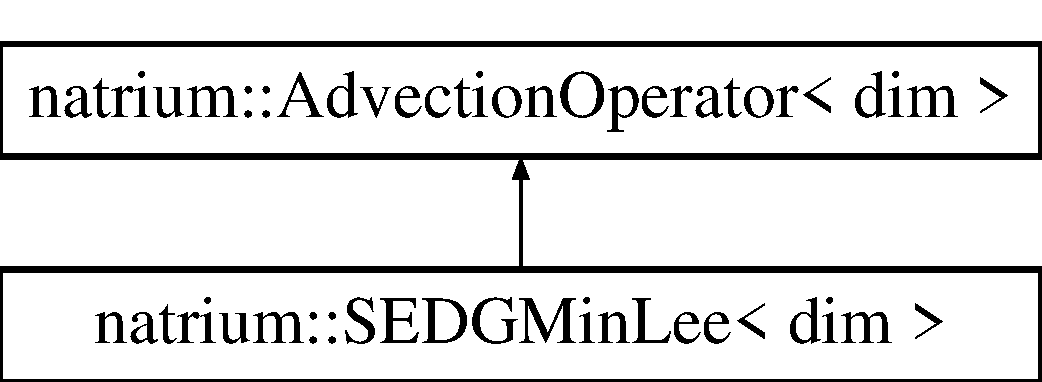
\includegraphics[height=2.000000cm]{classnatrium_1_1AdvectionOperator}
\end{center}
\end{figure}
\subsection*{Public Member Functions}
\begin{DoxyCompactItemize}
\item 
\hypertarget{classnatrium_1_1AdvectionOperator_a48d3a57e3433d9f6c3768ad2f392df56}{\hyperlink{classnatrium_1_1AdvectionOperator_a48d3a57e3433d9f6c3768ad2f392df56}{Advection\-Operator} ()}\label{classnatrium_1_1AdvectionOperator_a48d3a57e3433d9f6c3768ad2f392df56}

\begin{DoxyCompactList}\small\item\em constructor \end{DoxyCompactList}\item 
\hypertarget{classnatrium_1_1AdvectionOperator_a691156dace41e3075fd89953f30ae83f}{virtual \hyperlink{classnatrium_1_1AdvectionOperator_a691156dace41e3075fd89953f30ae83f}{$\sim$\-Advection\-Operator} ()}\label{classnatrium_1_1AdvectionOperator_a691156dace41e3075fd89953f30ae83f}

\begin{DoxyCompactList}\small\item\em destructor \end{DoxyCompactList}\item 
\hypertarget{classnatrium_1_1AdvectionOperator_a89c25c3dae9a1e5973cd89fab8c2c052}{virtual void \hyperlink{classnatrium_1_1AdvectionOperator_a89c25c3dae9a1e5973cd89fab8c2c052}{reassemble} ()=0}\label{classnatrium_1_1AdvectionOperator_a89c25c3dae9a1e5973cd89fab8c2c052}

\begin{DoxyCompactList}\small\item\em function to (re-\/)assemble linear system \end{DoxyCompactList}\item 
\hypertarget{classnatrium_1_1AdvectionOperator_aacdf6096f40166c5ec64686655c906a0}{virtual void \hyperlink{classnatrium_1_1AdvectionOperator_aacdf6096f40166c5ec64686655c906a0}{stream} ()=0}\label{classnatrium_1_1AdvectionOperator_aacdf6096f40166c5ec64686655c906a0}

\begin{DoxyCompactList}\small\item\em make streaming step \end{DoxyCompactList}\item 
\hypertarget{classnatrium_1_1AdvectionOperator_a2cbaee43740d976492e6c9d6d2b84ad0}{virtual const \\*
distributed\-\_\-sparse\-\_\-block\-\_\-matrix \& {\bfseries get\-System\-Matrix} () const =0}\label{classnatrium_1_1AdvectionOperator_a2cbaee43740d976492e6c9d6d2b84ad0}

\item 
\hypertarget{classnatrium_1_1AdvectionOperator_aa1eb5cd5a2c1b6b3b8f6395bac67ef55}{virtual const \\*
distributed\-\_\-block\-\_\-vector \& {\bfseries get\-System\-Vector} () const =0}\label{classnatrium_1_1AdvectionOperator_aa1eb5cd5a2c1b6b3b8f6395bac67ef55}

\item 
\hypertarget{classnatrium_1_1AdvectionOperator_a68f51edd8cc34b61f32ded0a8db82f7b}{virtual const shared\-\_\-ptr\\*
$<$ dealii\-::\-Do\-F\-Handler$<$ dim $>$ $>$ \& {\bfseries get\-Do\-F\-Handler} () const =0}\label{classnatrium_1_1AdvectionOperator_a68f51edd8cc34b61f32ded0a8db82f7b}

\item 
\hypertarget{classnatrium_1_1AdvectionOperator_adc118010e30df45b5906d35743e5ec2e}{virtual void {\bfseries map\-Do\-Fs\-To\-Support\-Points} (vector$<$ dealii\-::\-Point$<$ dim $>$ $>$ \&support\-Points) const =0}\label{classnatrium_1_1AdvectionOperator_adc118010e30df45b5906d35743e5ec2e}

\item 
\hypertarget{classnatrium_1_1AdvectionOperator_a419e94f5534d7871cee47c027a2501c4}{virtual const \\*
dealii\-::\-Mapping\-Q1$<$ dim $>$ \& {\bfseries get\-Mapping} () const =0}\label{classnatrium_1_1AdvectionOperator_a419e94f5534d7871cee47c027a2501c4}

\item 
virtual void \hyperlink{classnatrium_1_1AdvectionOperator_aca14260bae100874b0050a2a96d7a564}{save\-Checkpoint} (const string \&directory) const =0
\begin{DoxyCompactList}\small\item\em save matrices and status to files \end{DoxyCompactList}\item 
\hypertarget{classnatrium_1_1AdvectionOperator_a251e21d1dd023926d4c5f7fd973b90bf}{virtual size\-\_\-t {\bfseries get\-Number\-Of\-Do\-Fs} () const =0}\label{classnatrium_1_1AdvectionOperator_a251e21d1dd023926d4c5f7fd973b90bf}

\end{DoxyCompactItemize}


\subsection{Detailed Description}
\subsubsection*{template$<$size\-\_\-t dim$>$class natrium\-::\-Advection\-Operator$<$ dim $>$}

Abstract class for spatial part of the Advection Operator e\-\_\-i $\ast$ dx\-\_\-i f. 


\begin{DoxyTemplParams}{Template Parameters}
{\em dim} & The dimension of the flow (2 or 3). \\
\hline
\end{DoxyTemplParams}


\subsection{Member Function Documentation}
\hypertarget{classnatrium_1_1AdvectionOperator_aca14260bae100874b0050a2a96d7a564}{\index{natrium\-::\-Advection\-Operator@{natrium\-::\-Advection\-Operator}!save\-Checkpoint@{save\-Checkpoint}}
\index{save\-Checkpoint@{save\-Checkpoint}!natrium::AdvectionOperator@{natrium\-::\-Advection\-Operator}}
\subsubsection[{save\-Checkpoint}]{\setlength{\rightskip}{0pt plus 5cm}template$<$size\-\_\-t dim$>$ virtual void {\bf natrium\-::\-Advection\-Operator}$<$ dim $>$\-::save\-Checkpoint (
\begin{DoxyParamCaption}
\item[{const string \&}]{directory}
\end{DoxyParamCaption}
) const\hspace{0.3cm}{\ttfamily [pure virtual]}}}\label{classnatrium_1_1AdvectionOperator_aca14260bae100874b0050a2a96d7a564}


save matrices and status to files 


\begin{DoxyParams}[1]{Parameters}
\mbox{\tt in}  & {\em directory} & directory to save the matrix files to \\
\hline
\end{DoxyParams}

\begin{DoxyExceptions}{Exceptions}
{\em \hyperlink{classnatrium_1_1AdvectionSolverException}{Advection\-Solver\-Exception}} & \\
\hline
\end{DoxyExceptions}


Implemented in \hyperlink{classnatrium_1_1SEDGMinLee_ab3cf80e18230ee7f08f4ed9883b9dadd}{natrium\-::\-S\-E\-D\-G\-Min\-Lee$<$ dim $>$}.



The documentation for this class was generated from the following file\-:\begin{DoxyCompactItemize}
\item 
/home/kraemer/eclipse\-\_\-workspace/\-N\-A\-Triu\-M/src/natrium/advection/\hyperlink{AdvectionOperator_8h}{Advection\-Operator.\-h}\end{DoxyCompactItemize}

\hypertarget{classnatrium_1_1AdvectionSolverException}{
\section{natrium::AdvectionSolverException Class Reference}
\label{classnatrium_1_1AdvectionSolverException}\index{natrium::AdvectionSolverException@{natrium::AdvectionSolverException}}
}


Exception class for \hyperlink{classnatrium_1_1AdvectionOperator}{AdvectionOperator}.  


{\ttfamily \#include $<$AdvectionTools.h$>$}Inheritance diagram for natrium::AdvectionSolverException::\begin{figure}[H]
\begin{center}
\leavevmode
\includegraphics[height=2cm]{classnatrium_1_1AdvectionSolverException}
\end{center}
\end{figure}
\subsection*{Public Member Functions}
\begin{DoxyCompactItemize}
\item 
\hypertarget{classnatrium_1_1AdvectionSolverException_a443084a12dee879bdfbfc900202a0706}{
{\bfseries AdvectionSolverException} (const char $\ast$msg)}
\label{classnatrium_1_1AdvectionSolverException_a443084a12dee879bdfbfc900202a0706}

\item 
\hypertarget{classnatrium_1_1AdvectionSolverException_a9cda3faa279e3528f96c3780a91545bd}{
{\bfseries AdvectionSolverException} (const string \&msg)}
\label{classnatrium_1_1AdvectionSolverException_a9cda3faa279e3528f96c3780a91545bd}

\item 
\hypertarget{classnatrium_1_1AdvectionSolverException_aeb13fafe3f75de7cfd4e282a8a0fb5b0}{
const char $\ast$ {\bfseries what} () const   throw ()}
\label{classnatrium_1_1AdvectionSolverException_aeb13fafe3f75de7cfd4e282a8a0fb5b0}

\end{DoxyCompactItemize}


\subsection{Detailed Description}
Exception class for \hyperlink{classnatrium_1_1AdvectionOperator}{AdvectionOperator}. 

The documentation for this class was generated from the following file:\begin{DoxyCompactItemize}
\item 
/mnt/fdrive/akraem3m/workspace/NATriuM/src/library/natrium/advection/AdvectionTools.h\end{DoxyCompactItemize}

\hypertarget{classnatrium_1_1BGKTransformed}{\section{natrium\-:\-:B\-G\-K\-Transformed Class Reference}
\label{classnatrium_1_1BGKTransformed}\index{natrium\-::\-B\-G\-K\-Transformed@{natrium\-::\-B\-G\-K\-Transformed}}
}


Description of the B\-G\-K model for the transformed particle distributions, as described in Global data which is used by Min and Lee (2011)\-: A spectral-\/element discontinuous Galerkin lattice Boltzmann method for nearly incompressible flows, J\-C\-P 230 pp. 245-\/259.  




{\ttfamily \#include $<$B\-G\-K\-Transformed.\-h$>$}

Inheritance diagram for natrium\-:\-:B\-G\-K\-Transformed\-:\begin{figure}[H]
\begin{center}
\leavevmode
\includegraphics[height=2.000000cm]{classnatrium_1_1BGKTransformed}
\end{center}
\end{figure}
\subsection*{Public Member Functions}
\begin{DoxyCompactItemize}
\item 
\hyperlink{classnatrium_1_1BGKTransformed_aafd0ed5b888da93e496c0a29e092bf5b}{B\-G\-K\-Transformed} (double relaxation\-Parameter, boost\-::shared\-\_\-ptr$<$ \hyperlink{classnatrium_1_1BoltzmannModel}{Boltzmann\-Model} $>$ boltzmann\-Model)
\begin{DoxyCompactList}\small\item\em constructor \end{DoxyCompactList}\item 
\hypertarget{classnatrium_1_1BGKTransformed_a554c68facfbd2b126f24504f215eb193}{virtual \hyperlink{classnatrium_1_1BGKTransformed_a554c68facfbd2b126f24504f215eb193}{$\sim$\-B\-G\-K\-Transformed} ()}\label{classnatrium_1_1BGKTransformed_a554c68facfbd2b126f24504f215eb193}

\begin{DoxyCompactList}\small\item\em destructor \end{DoxyCompactList}\item 
virtual void \hyperlink{classnatrium_1_1BGKTransformed_a2e40159e5f5204431b1acb84b15910c0}{collide\-Single\-Point} (vector$<$ double $>$ \&distributions) const 
\begin{DoxyCompactList}\small\item\em function for collision \end{DoxyCompactList}\item 
virtual void \hyperlink{classnatrium_1_1BGKTransformed_a6bb41acd37234d2f92a9d868ff2486e1}{collide\-Single\-Do\-F} (size\-\_\-t do\-F, const vector$<$ double $>$ \&feq, \hyperlink{classnatrium_1_1DistributionFunctions}{Distribution\-Functions} \&f) const 
\begin{DoxyCompactList}\small\item\em virtual function for collision \end{DoxyCompactList}\end{DoxyCompactItemize}
\subsection*{Additional Inherited Members}


\subsection{Detailed Description}
Description of the B\-G\-K model for the transformed particle distributions, as described in Global data which is used by Min and Lee (2011)\-: A spectral-\/element discontinuous Galerkin lattice Boltzmann method for nearly incompressible flows, J\-C\-P 230 pp. 245-\/259. 

\subsection{Constructor \& Destructor Documentation}
\hypertarget{classnatrium_1_1BGKTransformed_aafd0ed5b888da93e496c0a29e092bf5b}{\index{natrium\-::\-B\-G\-K\-Transformed@{natrium\-::\-B\-G\-K\-Transformed}!B\-G\-K\-Transformed@{B\-G\-K\-Transformed}}
\index{B\-G\-K\-Transformed@{B\-G\-K\-Transformed}!natrium::BGKTransformed@{natrium\-::\-B\-G\-K\-Transformed}}
\subsubsection[{B\-G\-K\-Transformed}]{\setlength{\rightskip}{0pt plus 5cm}natrium\-::\-B\-G\-K\-Transformed\-::\-B\-G\-K\-Transformed (
\begin{DoxyParamCaption}
\item[{double}]{relaxation\-Parameter, }
\item[{boost\-::shared\-\_\-ptr$<$ {\bf Boltzmann\-Model} $>$}]{boltzmann\-Model}
\end{DoxyParamCaption}
)}}\label{classnatrium_1_1BGKTransformed_aafd0ed5b888da93e496c0a29e092bf5b}


constructor 


\begin{DoxyParams}[1]{Parameters}
\mbox{\tt in}  & {\em relaxation\-Parameter} & relaxation parameter tau \\
\hline
\end{DoxyParams}


\subsection{Member Function Documentation}
\hypertarget{classnatrium_1_1BGKTransformed_a6bb41acd37234d2f92a9d868ff2486e1}{\index{natrium\-::\-B\-G\-K\-Transformed@{natrium\-::\-B\-G\-K\-Transformed}!collide\-Single\-Do\-F@{collide\-Single\-Do\-F}}
\index{collide\-Single\-Do\-F@{collide\-Single\-Do\-F}!natrium::BGKTransformed@{natrium\-::\-B\-G\-K\-Transformed}}
\subsubsection[{collide\-Single\-Do\-F}]{\setlength{\rightskip}{0pt plus 5cm}void natrium\-::\-B\-G\-K\-Transformed\-::collide\-Single\-Do\-F (
\begin{DoxyParamCaption}
\item[{size\-\_\-t}]{do\-F, }
\item[{const vector$<$ double $>$ \&}]{feq, }
\item[{{\bf Distribution\-Functions} \&}]{f}
\end{DoxyParamCaption}
) const\hspace{0.3cm}{\ttfamily [virtual]}}}\label{classnatrium_1_1BGKTransformed_a6bb41acd37234d2f92a9d868ff2486e1}


virtual function for collision 


\begin{DoxyParams}[1]{Parameters}
\mbox{\tt in}  & {\em do\-F} & the do\-F index for which collision is done \\
\hline
\mbox{\tt in}  & {\em feq} & the vector of local equilibrium distributions \\
\hline
\mbox{\tt in}  & {\em f} & the vector of global distribution functions \\
\hline
\end{DoxyParams}


Implements \hyperlink{classnatrium_1_1CollisionModel_abe4f58658074680b679db7b7fddd6113}{natrium\-::\-Collision\-Model}.

\hypertarget{classnatrium_1_1BGKTransformed_a2e40159e5f5204431b1acb84b15910c0}{\index{natrium\-::\-B\-G\-K\-Transformed@{natrium\-::\-B\-G\-K\-Transformed}!collide\-Single\-Point@{collide\-Single\-Point}}
\index{collide\-Single\-Point@{collide\-Single\-Point}!natrium::BGKTransformed@{natrium\-::\-B\-G\-K\-Transformed}}
\subsubsection[{collide\-Single\-Point}]{\setlength{\rightskip}{0pt plus 5cm}void natrium\-::\-B\-G\-K\-Transformed\-::collide\-Single\-Point (
\begin{DoxyParamCaption}
\item[{vector$<$ double $>$ \&}]{distributions}
\end{DoxyParamCaption}
) const\hspace{0.3cm}{\ttfamily [virtual]}}}\label{classnatrium_1_1BGKTransformed_a2e40159e5f5204431b1acb84b15910c0}


function for collision 


\begin{DoxyParams}{Parameters}
{\em in/out\mbox{]}} & distributions the particle distribution functions \\
\hline
\end{DoxyParams}


Implements \hyperlink{classnatrium_1_1CollisionModel_acde767e924eb2124ab3eb725543111e8}{natrium\-::\-Collision\-Model}.



The documentation for this class was generated from the following files\-:\begin{DoxyCompactItemize}
\item 
/home/kraemer/eclipse\-\_\-workspace/\-N\-A\-Triu\-M/src/natrium/collisionmodels/\hyperlink{BGKTransformed_8h}{B\-G\-K\-Transformed.\-h}\item 
/home/kraemer/eclipse\-\_\-workspace/\-N\-A\-Triu\-M/src/natrium/collisionmodels/\hyperlink{BGKTransformed_8cpp}{B\-G\-K\-Transformed.\-cpp}\end{DoxyCompactItemize}

\hypertarget{classnatrium_1_1BoltzmannModel}{\section{natrium\-:\-:\-Boltzmann\-Model \-Class \-Reference}
\label{classnatrium_1_1BoltzmannModel}\index{natrium\-::\-Boltzmann\-Model@{natrium\-::\-Boltzmann\-Model}}
}


\-Abstract class for the description of a boltzmann model, e.\-g. \-D2\-Q9.  




{\ttfamily \#include $<$\-Boltzmann\-Model.\-h$>$}

\-Inheritance diagram for natrium\-:\-:\-Boltzmann\-Model\-:\begin{figure}[H]
\begin{center}
\leavevmode
\includegraphics[height=3.000000cm]{classnatrium_1_1BoltzmannModel}
\end{center}
\end{figure}
\subsection*{\-Public \-Member \-Functions}
\begin{DoxyCompactItemize}
\item 
\hyperlink{classnatrium_1_1BoltzmannModel_a0547ee3c88330d7a2ac44ad3ece8d560}{\-Boltzmann\-Model} (size\-\_\-t d, size\-\_\-t q, const vector$<$ numeric\-\_\-vector $>$ \&directions, const vector$<$ float\-\_\-t $>$ \&weights, \-Stencil\-Type stencil\-Type)
\begin{DoxyCompactList}\small\item\em constructor \end{DoxyCompactList}\item 
\hypertarget{classnatrium_1_1BoltzmannModel_ac2e3dabcbe15c1e37ff09ec1c53dafa5}{virtual \hyperlink{classnatrium_1_1BoltzmannModel_ac2e3dabcbe15c1e37ff09ec1c53dafa5}{$\sim$\-Boltzmann\-Model} ()}\label{classnatrium_1_1BoltzmannModel_ac2e3dabcbe15c1e37ff09ec1c53dafa5}

\begin{DoxyCompactList}\small\item\em destructor \end{DoxyCompactList}\item 
const vector$<$ numeric\-\_\-vector $>$ \& \hyperlink{classnatrium_1_1BoltzmannModel_aeabed4142acd04a57ba41ca26dfbe666}{get\-Directions} () const 
\begin{DoxyCompactList}\small\item\em get a reference to the vector of directions \end{DoxyCompactList}\item 
const numeric\-\_\-vector \& \hyperlink{classnatrium_1_1BoltzmannModel_a0b258b2c7cc4cba5ac666a06ca2a8f49}{get\-Direction} (size\-\_\-t i) const 
\begin{DoxyCompactList}\small\item\em get the i-\/th direction \end{DoxyCompactList}\item 
size\-\_\-t \hyperlink{classnatrium_1_1BoltzmannModel_ae7cfcd108a085d3215cdc8c00e826107}{get\-Q} () const 
\begin{DoxyCompactList}\small\item\em get q, the number of directions in the \-Dd\-Qq-\/stencil \end{DoxyCompactList}\item 
size\-\_\-t \hyperlink{classnatrium_1_1BoltzmannModel_a8d16745a0dab65cb0324d6b076e53d15}{get\-D} () const 
\begin{DoxyCompactList}\small\item\em get d, the dimension of the \-Dd\-Qq-\/stencil \end{DoxyCompactList}\item 
const vector$<$ float\-\_\-t $>$ \& \hyperlink{classnatrium_1_1BoltzmannModel_a3158e70071707c169486d87d26727f3c}{get\-Weights} () const 
\begin{DoxyCompactList}\small\item\em get the weights of the equilibrium distributions \end{DoxyCompactList}\item 
float\-\_\-t \hyperlink{classnatrium_1_1BoltzmannModel_aae549c1f5dd48a92fc9e174afc5de1a5}{get\-Weight} (size\-\_\-t i) const 
\begin{DoxyCompactList}\small\item\em get the weight belonging to a certain direction \end{DoxyCompactList}\item 
const \-Stencil\-Type \hyperlink{classnatrium_1_1BoltzmannModel_ac95c2547a37e380d8d7b3de3c0f8a4c2}{get\-Stencil\-Type} () const 
\begin{DoxyCompactList}\small\item\em get stencil type \end{DoxyCompactList}\item 
float\-\_\-t \hyperlink{classnatrium_1_1BoltzmannModel_adf8901da899eef5d11b0cbf80200ee32}{calculate\-Density} (const vector$<$ float\-\_\-t $>$ \&distributions) const 
\begin{DoxyCompactList}\small\item\em calculate macroscopic density \end{DoxyCompactList}\item 
numeric\-\_\-vector \hyperlink{classnatrium_1_1BoltzmannModel_a2c7e3465bb3541e420f15a7970533047}{calculate\-Velocity} (const vector$<$ float\-\_\-t $>$ \&distributions) const 
\begin{DoxyCompactList}\small\item\em calculate macroscopic velocity \end{DoxyCompactList}\item 
void \hyperlink{classnatrium_1_1BoltzmannModel_a3d5a504ad3dc0b3847c5db412b1988b8}{calculate\-Velocity} (const vector$<$ float\-\_\-t $>$ \&distributions, const float\-\_\-t rho, numeric\-\_\-vector \&u) const 
\begin{DoxyCompactList}\small\item\em calculate macroscopic velocity; saves the double calculation of the density \end{DoxyCompactList}\item 
virtual float\-\_\-t \hyperlink{classnatrium_1_1BoltzmannModel_ac5615f43cd5c03c881734d4826ce31be}{get\-Equilibrium\-Distribution} (size\-\_\-t i, const numeric\-\_\-vector \&u, const float\-\_\-t rho=1) const =0
\begin{DoxyCompactList}\small\item\em virtual function for the calculation of the equilibrium distribution \end{DoxyCompactList}\item 
virtual void \hyperlink{classnatrium_1_1BoltzmannModel_aab8d824211e65a394536333c5537b325}{get\-Equilibrium\-Distributions} (vector$<$ float\-\_\-t $>$ \&feq, const numeric\-\_\-vector \&u, const float\-\_\-t rho=1) const 
\begin{DoxyCompactList}\small\item\em function for the calculation of all equilibrium distributions \end{DoxyCompactList}\end{DoxyCompactItemize}


\subsection{\-Detailed \-Description}
\-Abstract class for the description of a boltzmann model, e.\-g. \-D2\-Q9. 

\subsection{\-Constructor \& \-Destructor \-Documentation}
\hypertarget{classnatrium_1_1BoltzmannModel_a0547ee3c88330d7a2ac44ad3ece8d560}{\index{natrium\-::\-Boltzmann\-Model@{natrium\-::\-Boltzmann\-Model}!\-Boltzmann\-Model@{\-Boltzmann\-Model}}
\index{\-Boltzmann\-Model@{\-Boltzmann\-Model}!natrium::BoltzmannModel@{natrium\-::\-Boltzmann\-Model}}
\subsubsection[{\-Boltzmann\-Model}]{\setlength{\rightskip}{0pt plus 5cm}{\bf natrium\-::\-Boltzmann\-Model\-::\-Boltzmann\-Model} (
\begin{DoxyParamCaption}
\item[{size\-\_\-t}]{d, }
\item[{size\-\_\-t}]{q, }
\item[{const vector$<$ numeric\-\_\-vector $>$ \&}]{directions, }
\item[{const vector$<$ float\-\_\-t $>$ \&}]{weights, }
\item[{\-Stencil\-Type}]{stencil\-Type}
\end{DoxyParamCaption}
)}}\label{classnatrium_1_1BoltzmannModel_a0547ee3c88330d7a2ac44ad3ece8d560}


constructor 


\begin{DoxyParams}{\-Parameters}
{\em d} & dimension \\
\hline
{\em q} & number of directions \\
\hline
{\em directions} & the directions of the stencil \\
\hline
{\em weights} & the weights of the equilibrium distribution \\
\hline
{\em stencil\-Type} & type of the stencil (e.\-g. \-D2\-Q9) \\
\hline
\end{DoxyParams}


\subsection{\-Member \-Function \-Documentation}
\hypertarget{classnatrium_1_1BoltzmannModel_adf8901da899eef5d11b0cbf80200ee32}{\index{natrium\-::\-Boltzmann\-Model@{natrium\-::\-Boltzmann\-Model}!calculate\-Density@{calculate\-Density}}
\index{calculate\-Density@{calculate\-Density}!natrium::BoltzmannModel@{natrium\-::\-Boltzmann\-Model}}
\subsubsection[{calculate\-Density}]{\setlength{\rightskip}{0pt plus 5cm}float\-\_\-t {\bf natrium\-::\-Boltzmann\-Model\-::calculate\-Density} (
\begin{DoxyParamCaption}
\item[{const vector$<$ float\-\_\-t $>$ \&}]{distributions}
\end{DoxyParamCaption}
) const\hspace{0.3cm}{\ttfamily  \mbox{[}inline\mbox{]}}}}\label{classnatrium_1_1BoltzmannModel_adf8901da899eef5d11b0cbf80200ee32}


calculate macroscopic density 


\begin{DoxyParams}[1]{\-Parameters}
\mbox{\tt in}  & {\em distributions} & particle distribution functions at a given point \\
\hline
\end{DoxyParams}
\begin{DoxyReturn}{\-Returns}
macroscopic density (sum of all distributions) 
\end{DoxyReturn}
\hypertarget{classnatrium_1_1BoltzmannModel_a2c7e3465bb3541e420f15a7970533047}{\index{natrium\-::\-Boltzmann\-Model@{natrium\-::\-Boltzmann\-Model}!calculate\-Velocity@{calculate\-Velocity}}
\index{calculate\-Velocity@{calculate\-Velocity}!natrium::BoltzmannModel@{natrium\-::\-Boltzmann\-Model}}
\subsubsection[{calculate\-Velocity}]{\setlength{\rightskip}{0pt plus 5cm}numeric\-\_\-vector {\bf natrium\-::\-Boltzmann\-Model\-::calculate\-Velocity} (
\begin{DoxyParamCaption}
\item[{const vector$<$ float\-\_\-t $>$ \&}]{distributions}
\end{DoxyParamCaption}
) const\hspace{0.3cm}{\ttfamily  \mbox{[}inline\mbox{]}}}}\label{classnatrium_1_1BoltzmannModel_a2c7e3465bb3541e420f15a7970533047}


calculate macroscopic velocity 


\begin{DoxyParams}[1]{\-Parameters}
\mbox{\tt in}  & {\em distributions} & particle distribution functions at a given point \\
\hline
\end{DoxyParams}
\begin{DoxyReturn}{\-Returns}
macroscopic velocity 
\end{DoxyReturn}
\hypertarget{classnatrium_1_1BoltzmannModel_a3d5a504ad3dc0b3847c5db412b1988b8}{\index{natrium\-::\-Boltzmann\-Model@{natrium\-::\-Boltzmann\-Model}!calculate\-Velocity@{calculate\-Velocity}}
\index{calculate\-Velocity@{calculate\-Velocity}!natrium::BoltzmannModel@{natrium\-::\-Boltzmann\-Model}}
\subsubsection[{calculate\-Velocity}]{\setlength{\rightskip}{0pt plus 5cm}void {\bf natrium\-::\-Boltzmann\-Model\-::calculate\-Velocity} (
\begin{DoxyParamCaption}
\item[{const vector$<$ float\-\_\-t $>$ \&}]{distributions, }
\item[{const float\-\_\-t}]{rho, }
\item[{numeric\-\_\-vector \&}]{u}
\end{DoxyParamCaption}
) const\hspace{0.3cm}{\ttfamily  \mbox{[}inline\mbox{]}}}}\label{classnatrium_1_1BoltzmannModel_a3d5a504ad3dc0b3847c5db412b1988b8}


calculate macroscopic velocity; saves the double calculation of the density 

\begin{DoxyNote}{\-Note}
more efficient 
\end{DoxyNote}

\begin{DoxyParams}[1]{\-Parameters}
\mbox{\tt in}  & {\em distributions} & particle distribution functions at a given point \\
\hline
\mbox{\tt in}  & {\em rho} & macroscopic density \\
\hline
\mbox{\tt out}  & {\em u} & macroscopic velocity \\
\hline
\end{DoxyParams}
\hypertarget{classnatrium_1_1BoltzmannModel_a8d16745a0dab65cb0324d6b076e53d15}{\index{natrium\-::\-Boltzmann\-Model@{natrium\-::\-Boltzmann\-Model}!get\-D@{get\-D}}
\index{get\-D@{get\-D}!natrium::BoltzmannModel@{natrium\-::\-Boltzmann\-Model}}
\subsubsection[{get\-D}]{\setlength{\rightskip}{0pt plus 5cm}size\-\_\-t {\bf natrium\-::\-Boltzmann\-Model\-::get\-D} (
\begin{DoxyParamCaption}
{}
\end{DoxyParamCaption}
) const\hspace{0.3cm}{\ttfamily  \mbox{[}inline\mbox{]}}}}\label{classnatrium_1_1BoltzmannModel_a8d16745a0dab65cb0324d6b076e53d15}


get d, the dimension of the \-Dd\-Qq-\/stencil 

\begin{DoxyReturn}{\-Returns}
d 
\end{DoxyReturn}
\hypertarget{classnatrium_1_1BoltzmannModel_a0b258b2c7cc4cba5ac666a06ca2a8f49}{\index{natrium\-::\-Boltzmann\-Model@{natrium\-::\-Boltzmann\-Model}!get\-Direction@{get\-Direction}}
\index{get\-Direction@{get\-Direction}!natrium::BoltzmannModel@{natrium\-::\-Boltzmann\-Model}}
\subsubsection[{get\-Direction}]{\setlength{\rightskip}{0pt plus 5cm}const numeric\-\_\-vector\& {\bf natrium\-::\-Boltzmann\-Model\-::get\-Direction} (
\begin{DoxyParamCaption}
\item[{size\-\_\-t}]{i}
\end{DoxyParamCaption}
) const\hspace{0.3cm}{\ttfamily  \mbox{[}inline\mbox{]}}}}\label{classnatrium_1_1BoltzmannModel_a0b258b2c7cc4cba5ac666a06ca2a8f49}


get the i-\/th direction 


\begin{DoxyParams}{\-Parameters}
{\em i} & index i \\
\hline
\end{DoxyParams}
\begin{DoxyReturn}{\-Returns}
a reference to the i-\/th direction of the \-Dd\-Qq-\/stencil 
\end{DoxyReturn}
\hypertarget{classnatrium_1_1BoltzmannModel_aeabed4142acd04a57ba41ca26dfbe666}{\index{natrium\-::\-Boltzmann\-Model@{natrium\-::\-Boltzmann\-Model}!get\-Directions@{get\-Directions}}
\index{get\-Directions@{get\-Directions}!natrium::BoltzmannModel@{natrium\-::\-Boltzmann\-Model}}
\subsubsection[{get\-Directions}]{\setlength{\rightskip}{0pt plus 5cm}const vector$<$numeric\-\_\-vector$>$\& {\bf natrium\-::\-Boltzmann\-Model\-::get\-Directions} (
\begin{DoxyParamCaption}
{}
\end{DoxyParamCaption}
) const\hspace{0.3cm}{\ttfamily  \mbox{[}inline\mbox{]}}}}\label{classnatrium_1_1BoltzmannModel_aeabed4142acd04a57ba41ca26dfbe666}


get a reference to the vector of directions 

\begin{DoxyReturn}{\-Returns}
a ublas\-\_\-vector, which contains the directions of the \-Dd\-Qq-\/stencil as ublas\-\_\-vectors 
\end{DoxyReturn}
\hypertarget{classnatrium_1_1BoltzmannModel_ac5615f43cd5c03c881734d4826ce31be}{\index{natrium\-::\-Boltzmann\-Model@{natrium\-::\-Boltzmann\-Model}!get\-Equilibrium\-Distribution@{get\-Equilibrium\-Distribution}}
\index{get\-Equilibrium\-Distribution@{get\-Equilibrium\-Distribution}!natrium::BoltzmannModel@{natrium\-::\-Boltzmann\-Model}}
\subsubsection[{get\-Equilibrium\-Distribution}]{\setlength{\rightskip}{0pt plus 5cm}virtual float\-\_\-t {\bf natrium\-::\-Boltzmann\-Model\-::get\-Equilibrium\-Distribution} (
\begin{DoxyParamCaption}
\item[{size\-\_\-t}]{i, }
\item[{const numeric\-\_\-vector \&}]{u, }
\item[{const float\-\_\-t}]{rho = {\ttfamily 1}}
\end{DoxyParamCaption}
) const\hspace{0.3cm}{\ttfamily  \mbox{[}pure virtual\mbox{]}}}}\label{classnatrium_1_1BoltzmannModel_ac5615f43cd5c03c881734d4826ce31be}


virtual function for the calculation of the equilibrium distribution 


\begin{DoxyParams}{\-Parameters}
{\em i} & index of the direction \\
\hline
{\em u} & macroscopic velocity \\
\hline
{\em rho} & macroscopic density \\
\hline
\end{DoxyParams}
\begin{DoxyReturn}{\-Returns}
value of the equilibrium distribution 
\end{DoxyReturn}
\begin{DoxyNote}{\-Note}
\-The calculation can surely be done more efficiently by passing different arguments, e.\-g. u$\ast$u or u/(c$^\wedge$2) 
\end{DoxyNote}


\-Implemented in \hyperlink{classnatrium_1_1D2Q9IncompressibleModel_a437bce6e0d6f35ca3ff2df4bbe650043}{natrium\-::\-D2\-Q9\-Incompressible\-Model}.

\hypertarget{classnatrium_1_1BoltzmannModel_aab8d824211e65a394536333c5537b325}{\index{natrium\-::\-Boltzmann\-Model@{natrium\-::\-Boltzmann\-Model}!get\-Equilibrium\-Distributions@{get\-Equilibrium\-Distributions}}
\index{get\-Equilibrium\-Distributions@{get\-Equilibrium\-Distributions}!natrium::BoltzmannModel@{natrium\-::\-Boltzmann\-Model}}
\subsubsection[{get\-Equilibrium\-Distributions}]{\setlength{\rightskip}{0pt plus 5cm}void {\bf natrium\-::\-Boltzmann\-Model\-::get\-Equilibrium\-Distributions} (
\begin{DoxyParamCaption}
\item[{vector$<$ float\-\_\-t $>$ \&}]{feq, }
\item[{const numeric\-\_\-vector \&}]{u, }
\item[{const float\-\_\-t}]{rho = {\ttfamily 1}}
\end{DoxyParamCaption}
) const\hspace{0.3cm}{\ttfamily  \mbox{[}virtual\mbox{]}}}}\label{classnatrium_1_1BoltzmannModel_aab8d824211e65a394536333c5537b325}


function for the calculation of all equilibrium distributions 


\begin{DoxyParams}[1]{\-Parameters}
\mbox{\tt out}  & {\em feq} & vector of all equality distributions, must have size \-Q \\
\hline
\mbox{\tt in}  & {\em u} & macroscopic velocity \\
\hline
\mbox{\tt in}  & {\em rho} & macroscopic density \\
\hline
\end{DoxyParams}
\begin{DoxyNote}{\-Note}
\-The calculation can surely be done more efficiently by passing different arguments, e.\-g. u$\ast$u or u/(c$^\wedge$2) 
\end{DoxyNote}
\hypertarget{classnatrium_1_1BoltzmannModel_ae7cfcd108a085d3215cdc8c00e826107}{\index{natrium\-::\-Boltzmann\-Model@{natrium\-::\-Boltzmann\-Model}!get\-Q@{get\-Q}}
\index{get\-Q@{get\-Q}!natrium::BoltzmannModel@{natrium\-::\-Boltzmann\-Model}}
\subsubsection[{get\-Q}]{\setlength{\rightskip}{0pt plus 5cm}size\-\_\-t {\bf natrium\-::\-Boltzmann\-Model\-::get\-Q} (
\begin{DoxyParamCaption}
{}
\end{DoxyParamCaption}
) const\hspace{0.3cm}{\ttfamily  \mbox{[}inline\mbox{]}}}}\label{classnatrium_1_1BoltzmannModel_ae7cfcd108a085d3215cdc8c00e826107}


get q, the number of directions in the \-Dd\-Qq-\/stencil 

\begin{DoxyReturn}{\-Returns}
q 
\end{DoxyReturn}
\hypertarget{classnatrium_1_1BoltzmannModel_ac95c2547a37e380d8d7b3de3c0f8a4c2}{\index{natrium\-::\-Boltzmann\-Model@{natrium\-::\-Boltzmann\-Model}!get\-Stencil\-Type@{get\-Stencil\-Type}}
\index{get\-Stencil\-Type@{get\-Stencil\-Type}!natrium::BoltzmannModel@{natrium\-::\-Boltzmann\-Model}}
\subsubsection[{get\-Stencil\-Type}]{\setlength{\rightskip}{0pt plus 5cm}const \-Stencil\-Type {\bf natrium\-::\-Boltzmann\-Model\-::get\-Stencil\-Type} (
\begin{DoxyParamCaption}
{}
\end{DoxyParamCaption}
) const\hspace{0.3cm}{\ttfamily  \mbox{[}inline\mbox{]}}}}\label{classnatrium_1_1BoltzmannModel_ac95c2547a37e380d8d7b3de3c0f8a4c2}


get stencil type 

\begin{DoxyReturn}{\-Returns}
stencil type, e.\-g. \-D2\-Q9 
\end{DoxyReturn}
\hypertarget{classnatrium_1_1BoltzmannModel_aae549c1f5dd48a92fc9e174afc5de1a5}{\index{natrium\-::\-Boltzmann\-Model@{natrium\-::\-Boltzmann\-Model}!get\-Weight@{get\-Weight}}
\index{get\-Weight@{get\-Weight}!natrium::BoltzmannModel@{natrium\-::\-Boltzmann\-Model}}
\subsubsection[{get\-Weight}]{\setlength{\rightskip}{0pt plus 5cm}float\-\_\-t {\bf natrium\-::\-Boltzmann\-Model\-::get\-Weight} (
\begin{DoxyParamCaption}
\item[{size\-\_\-t}]{i}
\end{DoxyParamCaption}
) const\hspace{0.3cm}{\ttfamily  \mbox{[}inline\mbox{]}}}}\label{classnatrium_1_1BoltzmannModel_aae549c1f5dd48a92fc9e174afc5de1a5}


get the weight belonging to a certain direction 


\begin{DoxyParams}{\-Parameters}
{\em i} & index i of the direction (1 $<$= i $<$= q) \\
\hline
\end{DoxyParams}
\begin{DoxyReturn}{\-Returns}
the i-\/th weight 
\end{DoxyReturn}
\hypertarget{classnatrium_1_1BoltzmannModel_a3158e70071707c169486d87d26727f3c}{\index{natrium\-::\-Boltzmann\-Model@{natrium\-::\-Boltzmann\-Model}!get\-Weights@{get\-Weights}}
\index{get\-Weights@{get\-Weights}!natrium::BoltzmannModel@{natrium\-::\-Boltzmann\-Model}}
\subsubsection[{get\-Weights}]{\setlength{\rightskip}{0pt plus 5cm}const vector$<$float\-\_\-t$>$\& {\bf natrium\-::\-Boltzmann\-Model\-::get\-Weights} (
\begin{DoxyParamCaption}
{}
\end{DoxyParamCaption}
) const\hspace{0.3cm}{\ttfamily  \mbox{[}inline\mbox{]}}}}\label{classnatrium_1_1BoltzmannModel_a3158e70071707c169486d87d26727f3c}


get the weights of the equilibrium distributions 

\begin{DoxyReturn}{\-Returns}
a reference to the vector of weights 
\end{DoxyReturn}


\-The documentation for this class was generated from the following files\-:\begin{DoxyCompactItemize}
\item 
/home/kraemer/eclipse\-\_\-workspace/\-N\-A\-Triu\-M/src/boltzmannmodels/\hyperlink{BoltzmannModel_8h}{\-Boltzmann\-Model.\-h}\item 
/home/kraemer/eclipse\-\_\-workspace/\-N\-A\-Triu\-M/src/boltzmannmodels/\hyperlink{BoltzmannModel_8cpp}{\-Boltzmann\-Model.\-cpp}\end{DoxyCompactItemize}

\hypertarget{classnatrium_1_1Boundary}{
\section{natrium::Boundary$<$ dim $>$ Class Template Reference}
\label{classnatrium_1_1Boundary}\index{natrium::Boundary@{natrium::Boundary}}
}


Abstract class for the description of boundaries. Base class of \hyperlink{classnatrium_1_1PeriodicBoundary}{PeriodicBoundary}, InflowBoundary, etc.  


{\ttfamily \#include $<$Boundary.h$>$}Inheritance diagram for natrium::Boundary$<$ dim $>$::\begin{figure}[H]
\begin{center}
\leavevmode
\includegraphics[height=3cm]{classnatrium_1_1Boundary}
\end{center}
\end{figure}
\subsection*{Public Member Functions}
\begin{DoxyCompactItemize}
\item 
\hypertarget{classnatrium_1_1Boundary_a987978143b16ef0bbadd2b465dc1882d}{
\hyperlink{classnatrium_1_1Boundary_a987978143b16ef0bbadd2b465dc1882d}{Boundary} ()}
\label{classnatrium_1_1Boundary_a987978143b16ef0bbadd2b465dc1882d}

\begin{DoxyCompactList}\small\item\em constructor \item\end{DoxyCompactList}\item 
\hypertarget{classnatrium_1_1Boundary_a63e8fb8ec44288b9145f819b515ae6d9}{
virtual \hyperlink{classnatrium_1_1Boundary_a63e8fb8ec44288b9145f819b515ae6d9}{$\sim$Boundary} ()}
\label{classnatrium_1_1Boundary_a63e8fb8ec44288b9145f819b515ae6d9}

\begin{DoxyCompactList}\small\item\em destructor \item\end{DoxyCompactList}\item 
\hypertarget{classnatrium_1_1Boundary_acb651f4148b4e00f08258e1321c43235}{
virtual bool \hyperlink{classnatrium_1_1Boundary_acb651f4148b4e00f08258e1321c43235}{isPeriodic} () const }
\label{classnatrium_1_1Boundary_acb651f4148b4e00f08258e1321c43235}

\begin{DoxyCompactList}\small\item\em is the boundary a periodic boundary ? \item\end{DoxyCompactList}\end{DoxyCompactItemize}


\subsection{Detailed Description}
\subsubsection*{template$<$size\_\-t dim$>$ class natrium::Boundary$<$ dim $>$}

Abstract class for the description of boundaries. Base class of \hyperlink{classnatrium_1_1PeriodicBoundary}{PeriodicBoundary}, InflowBoundary, etc. 
\begin{DoxyTemplParams}{Template Parameters}
\item[{\em dim}]The dimension of the boundary is the dimension of the domain -\/1 ( e.g. 2-\/dim meshes have 1-\/dim boundary) \end{DoxyTemplParams}


The documentation for this class was generated from the following file:\begin{DoxyCompactItemize}
\item 
/mnt/fdrive/akraem3m/workspace/NATriuM/src/library/natrium/problemdescription/\hyperlink{Boundary_8h}{Boundary.h}\end{DoxyCompactItemize}

\hypertarget{classnatrium_1_1BoundaryCollection}{\section{natrium\-:\-:Boundary\-Collection$<$ dim $>$ Class Template Reference}
\label{classnatrium_1_1BoundaryCollection}\index{natrium\-::\-Boundary\-Collection$<$ dim $>$@{natrium\-::\-Boundary\-Collection$<$ dim $>$}}
}
\subsection*{Public Member Functions}
\begin{DoxyCompactItemize}
\item 
\hypertarget{classnatrium_1_1BoundaryCollection_a60d5efd5fa9bf2107705ee1a38508dd4}{void {\bfseries add\-Boundary} (shared\-\_\-ptr$<$ \hyperlink{classnatrium_1_1PeriodicBoundary}{Periodic\-Boundary}$<$ dim $>$ $>$ boundary)}\label{classnatrium_1_1BoundaryCollection_a60d5efd5fa9bf2107705ee1a38508dd4}

\item 
\hypertarget{classnatrium_1_1BoundaryCollection_a89de2718a8813905dc1487f812e363a2}{void {\bfseries apply\-Boundaries} (const shared\-\_\-ptr$<$ dealii\-::\-Do\-F\-Handler$<$ dim $>$ $>$ do\-F\-Handler)}\label{classnatrium_1_1BoundaryCollection_a89de2718a8813905dc1487f812e363a2}

\item 
\hypertarget{classnatrium_1_1BoundaryCollection_a165425d13fc67c25f13c56ba49468102}{const vector$<$ shared\-\_\-ptr\\*
$<$ \hyperlink{classnatrium_1_1Boundary}{Boundary}$<$ dim $>$ $>$ $>$ \& {\bfseries get\-Boundaries} () const }\label{classnatrium_1_1BoundaryCollection_a165425d13fc67c25f13c56ba49468102}

\item 
\hypertarget{classnatrium_1_1BoundaryCollection_a1d7ac8cc1b11c7b241f16be4a41c4582}{const vector$<$ shared\-\_\-ptr\\*
$<$ \hyperlink{classnatrium_1_1PeriodicBoundary}{Periodic\-Boundary}$<$ dim $>$ $>$ $>$ \& {\bfseries get\-Periodic\-Boundaries} () const }\label{classnatrium_1_1BoundaryCollection_a1d7ac8cc1b11c7b241f16be4a41c4582}

\item 
\hypertarget{classnatrium_1_1BoundaryCollection_aaebf4e5f32663f1f94c08fdc9902c06f}{const size\-\_\-t {\bfseries number\-Of\-Boundaries} () const }\label{classnatrium_1_1BoundaryCollection_aaebf4e5f32663f1f94c08fdc9902c06f}

\item 
\hypertarget{classnatrium_1_1BoundaryCollection_a29d1d56e79872df40cbdd9a8150dd6d3}{const size\-\_\-t {\bfseries number\-Of\-Periodic\-Boundaries} () const }\label{classnatrium_1_1BoundaryCollection_a29d1d56e79872df40cbdd9a8150dd6d3}

\end{DoxyCompactItemize}


The documentation for this class was generated from the following file\-:\begin{DoxyCompactItemize}
\item 
/home/kraemer/eclipse\-\_\-workspace/\-N\-A\-Triu\-M/src/natrium/problemdescription/Boundary\-Collection.\-h\end{DoxyCompactItemize}

\hypertarget{classnatrium_1_1CFDSolver}{\section{natrium\-:\-:C\-F\-D\-Solver$<$ dim $>$ Class Template Reference}
\label{classnatrium_1_1CFDSolver}\index{natrium\-::\-C\-F\-D\-Solver$<$ dim $>$@{natrium\-::\-C\-F\-D\-Solver$<$ dim $>$}}
}


The central class for the C\-F\-D simulation based on the D\-B\-E.  




{\ttfamily \#include $<$C\-F\-D\-Solver.\-h$>$}

\subsection*{Public Member Functions}
\begin{DoxyCompactItemize}
\item 
\hyperlink{classnatrium_1_1CFDSolver_a2a459e7f9d5feb0d216f869812723af2}{C\-F\-D\-Solver} (shared\-\_\-ptr$<$ \hyperlink{classnatrium_1_1SolverConfiguration}{Solver\-Configuration} $>$ configuration, shared\-\_\-ptr$<$ \hyperlink{classnatrium_1_1ProblemDescription}{Problem\-Description}$<$ dim $>$ $>$ problem\-Description)
\item 
\hypertarget{classnatrium_1_1CFDSolver_a7ca9bd709255ac87b34f869c984b913b}{virtual \hyperlink{classnatrium_1_1CFDSolver_a7ca9bd709255ac87b34f869c984b913b}{$\sim$\-C\-F\-D\-Solver} ()}\label{classnatrium_1_1CFDSolver_a7ca9bd709255ac87b34f869c984b913b}

\begin{DoxyCompactList}\small\item\em destructor \end{DoxyCompactList}\item 
\hypertarget{classnatrium_1_1CFDSolver_abe627b0bbde0635abb30b9bea4c72dc1}{void \hyperlink{classnatrium_1_1CFDSolver_abe627b0bbde0635abb30b9bea4c72dc1}{initialize\-Distributions} ()}\label{classnatrium_1_1CFDSolver_abe627b0bbde0635abb30b9bea4c72dc1}

\begin{DoxyCompactList}\small\item\em initialize distribution functions \end{DoxyCompactList}\item 
\hypertarget{classnatrium_1_1CFDSolver_ac32a318e504b31195eb61c2cdc2659fe}{void \hyperlink{classnatrium_1_1CFDSolver_ac32a318e504b31195eb61c2cdc2659fe}{stream} ()}\label{classnatrium_1_1CFDSolver_ac32a318e504b31195eb61c2cdc2659fe}

\begin{DoxyCompactList}\small\item\em Advection in all directions. \end{DoxyCompactList}\item 
\hypertarget{classnatrium_1_1CFDSolver_ac9bec7d0c4bcd5e02c5213ec09438c02}{void \hyperlink{classnatrium_1_1CFDSolver_ac9bec7d0c4bcd5e02c5213ec09438c02}{collide} ()}\label{classnatrium_1_1CFDSolver_ac9bec7d0c4bcd5e02c5213ec09438c02}

\begin{DoxyCompactList}\small\item\em Low-\/level collide function. \end{DoxyCompactList}\item 
\hypertarget{classnatrium_1_1CFDSolver_a604212a1f6cd2549b8f60ab26b14de00}{void \hyperlink{classnatrium_1_1CFDSolver_a604212a1f6cd2549b8f60ab26b14de00}{reassemble} ()}\label{classnatrium_1_1CFDSolver_a604212a1f6cd2549b8f60ab26b14de00}

\begin{DoxyCompactList}\small\item\em reassembly of all matrices \end{DoxyCompactList}\item 
\hypertarget{classnatrium_1_1CFDSolver_a11f503bc3f3c306b240874c74a38025b}{void \hyperlink{classnatrium_1_1CFDSolver_a11f503bc3f3c306b240874c74a38025b}{run} ()}\label{classnatrium_1_1CFDSolver_a11f503bc3f3c306b240874c74a38025b}

\begin{DoxyCompactList}\small\item\em run C\-F\-D solver \end{DoxyCompactList}\item 
\hypertarget{classnatrium_1_1CFDSolver_abf6804f132885502b61877fc1f9ca4a2}{void \hyperlink{classnatrium_1_1CFDSolver_abf6804f132885502b61877fc1f9ca4a2}{output} (size\-\_\-t iteration)}\label{classnatrium_1_1CFDSolver_abf6804f132885502b61877fc1f9ca4a2}

\begin{DoxyCompactList}\small\item\em create output data and write to file \end{DoxyCompactList}\item 
\hypertarget{classnatrium_1_1CFDSolver_adf0b4e4da292bcb195d926d3174ba2a9}{const distributed\-\_\-vector \& {\bfseries get\-Density} () const }\label{classnatrium_1_1CFDSolver_adf0b4e4da292bcb195d926d3174ba2a9}

\item 
\hypertarget{classnatrium_1_1CFDSolver_aa7a6591ab785a87d60bcc12da9daf8ff}{const vector\\*
$<$ distributed\-\_\-vector $>$ \& {\bfseries get\-F} () const }\label{classnatrium_1_1CFDSolver_aa7a6591ab785a87d60bcc12da9daf8ff}

\item 
\hypertarget{classnatrium_1_1CFDSolver_a0e5ec3dc278216d5827410b7db82af59}{const vector\\*
$<$ distributed\-\_\-vector $>$ \& {\bfseries get\-Velocity} () const }\label{classnatrium_1_1CFDSolver_a0e5ec3dc278216d5827410b7db82af59}

\item 
\hypertarget{classnatrium_1_1CFDSolver_a1aea207c81089c2e46092489557bb139}{const shared\-\_\-ptr\\*
$<$ \hyperlink{classnatrium_1_1AdvectionOperator}{Advection\-Operator}$<$ dim $>$ $>$ \& {\bfseries get\-Advection\-Operator} () const }\label{classnatrium_1_1CFDSolver_a1aea207c81089c2e46092489557bb139}

\item 
\hypertarget{classnatrium_1_1CFDSolver_a3733dbd256b6d38659cee3cb044c1446}{const shared\-\_\-ptr\\*
$<$ \hyperlink{classnatrium_1_1BoltzmannModel}{Boltzmann\-Model} $>$ \& {\bfseries get\-Boltzmann\-Model} () const }\label{classnatrium_1_1CFDSolver_a3733dbd256b6d38659cee3cb044c1446}

\item 
\hypertarget{classnatrium_1_1CFDSolver_abb4b632b524bd68afcdff7d54c2d3d97}{const shared\-\_\-ptr\\*
$<$ \hyperlink{classnatrium_1_1CollisionModel}{Collision\-Model} $>$ \& {\bfseries get\-Collision\-Model} () const }\label{classnatrium_1_1CFDSolver_abb4b632b524bd68afcdff7d54c2d3d97}

\item 
\hypertarget{classnatrium_1_1CFDSolver_a413691491ac82f384a03293be2294de5}{const shared\-\_\-ptr\\*
$<$ \hyperlink{classnatrium_1_1SolverConfiguration}{Solver\-Configuration} $>$ \& {\bfseries get\-Configuration} () const }\label{classnatrium_1_1CFDSolver_a413691491ac82f384a03293be2294de5}

\item 
\hypertarget{classnatrium_1_1CFDSolver_a8b1131e8fd6b022bea5ddce72469c289}{const shared\-\_\-ptr\\*
$<$ \hyperlink{classnatrium_1_1ProblemDescription}{Problem\-Description}$<$ dim $>$ $>$ \& {\bfseries get\-Problem\-Description} () const }\label{classnatrium_1_1CFDSolver_a8b1131e8fd6b022bea5ddce72469c289}

\item 
\hypertarget{classnatrium_1_1CFDSolver_adc432b8516f531639914001616d36ab9}{const shared\-\_\-ptr\\*
$<$ \hyperlink{classnatrium_1_1TimeIntegrator}{Time\-Integrator}\\*
$<$ distributed\-\_\-vector, \\*
distributed\-\_\-sparse\-\_\-matrix $>$ $>$ \& {\bfseries get\-Time\-Integrator} () const }\label{classnatrium_1_1CFDSolver_adc432b8516f531639914001616d36ab9}

\item 
\hypertarget{classnatrium_1_1CFDSolver_a74d459ef4f43d42e04ceb2178bb006f4}{size\-\_\-t {\bfseries get\-Number\-Of\-Do\-Fs} () const }\label{classnatrium_1_1CFDSolver_a74d459ef4f43d42e04ceb2178bb006f4}

\item 
\hypertarget{classnatrium_1_1CFDSolver_ae9c44bb0f33e2c73ee96fbe100061842}{double {\bfseries get\-Max\-Velocity\-Norm} () const }\label{classnatrium_1_1CFDSolver_ae9c44bb0f33e2c73ee96fbe100061842}

\item 
\hypertarget{classnatrium_1_1CFDSolver_ade641431988a82cb47d88a9d600e1c92}{double {\bfseries get\-Max\-Density\-Deviation\-From} (double reference\-Density) const }\label{classnatrium_1_1CFDSolver_ade641431988a82cb47d88a9d600e1c92}

\item 
\hypertarget{classnatrium_1_1CFDSolver_a33c4bfd63b8d457a5bc15f0c0da02c38}{size\-\_\-t {\bfseries get\-Iteration\-Start} () const }\label{classnatrium_1_1CFDSolver_a33c4bfd63b8d457a5bc15f0c0da02c38}

\end{DoxyCompactItemize}
\subsection*{Protected Member Functions}
\begin{DoxyCompactItemize}
\item 
\hypertarget{classnatrium_1_1CFDSolver_a9a2592ea549fa10427c84f0a1e380c1e}{void \hyperlink{classnatrium_1_1CFDSolver_a9a2592ea549fa10427c84f0a1e380c1e}{save\-Distribution\-Functions\-To\-Files} (const string \&directory)}\label{classnatrium_1_1CFDSolver_a9a2592ea549fa10427c84f0a1e380c1e}

\begin{DoxyCompactList}\small\item\em save the distribution functions to files for checkpointing \end{DoxyCompactList}\item 
\hypertarget{classnatrium_1_1CFDSolver_a42245d22e289d079a3b06a0c26f50050}{void \hyperlink{classnatrium_1_1CFDSolver_a42245d22e289d079a3b06a0c26f50050}{load\-Distribution\-Functions\-From\-Files} (const string \&directory)}\label{classnatrium_1_1CFDSolver_a42245d22e289d079a3b06a0c26f50050}

\begin{DoxyCompactList}\small\item\em load the distribution functions from files for checkpointing \end{DoxyCompactList}\end{DoxyCompactItemize}


\subsection{Detailed Description}
\subsubsection*{template$<$size\-\_\-t dim$>$class natrium\-::\-C\-F\-D\-Solver$<$ dim $>$}

The central class for the C\-F\-D simulation based on the D\-B\-E. 

\begin{DoxyNote}{Note}
The \hyperlink{classnatrium_1_1CFDSolver}{C\-F\-D\-Solver} itself is quite static but it contains interchangeable modules, e.\-g. for the Boltzmann model or the time integrator. By these means, a variety of different simulation methods can be covered. 
\end{DoxyNote}

\begin{DoxyTemplParams}{Template Parameters}
{\em dim} & The dimension of the flow (2 or 3). \\
\hline
\end{DoxyTemplParams}


\subsection{Constructor \& Destructor Documentation}
\hypertarget{classnatrium_1_1CFDSolver_a2a459e7f9d5feb0d216f869812723af2}{\index{natrium\-::\-C\-F\-D\-Solver@{natrium\-::\-C\-F\-D\-Solver}!C\-F\-D\-Solver@{C\-F\-D\-Solver}}
\index{C\-F\-D\-Solver@{C\-F\-D\-Solver}!natrium::CFDSolver@{natrium\-::\-C\-F\-D\-Solver}}
\subsubsection[{C\-F\-D\-Solver}]{\setlength{\rightskip}{0pt plus 5cm}template$<$size\-\_\-t dim$>$ template {\bf natrium\-::\-C\-F\-D\-Solver}$<$ dim $>$\-::{\bf C\-F\-D\-Solver} (
\begin{DoxyParamCaption}
\item[{shared\-\_\-ptr$<$ {\bf Solver\-Configuration} $>$}]{configuration, }
\item[{shared\-\_\-ptr$<$ {\bf Problem\-Description}$<$ dim $>$ $>$}]{problem\-Description}
\end{DoxyParamCaption}
)}}\label{classnatrium_1_1CFDSolver_a2a459e7f9d5feb0d216f869812723af2}
constructor \begin{DoxyNote}{Note}
\-: has to be inlined, if the template parameter is not made explicit 
\end{DoxyNote}
check if problem and solver configuration fit together

Build boltzmann model

Build streaming data object

Calculate relaxation parameter and build collision model

Build time integrator 

The documentation for this class was generated from the following files\-:\begin{DoxyCompactItemize}
\item 
/home/kraemer/eclipse\-\_\-workspace/\-N\-A\-Triu\-M/src/natrium/solver/\hyperlink{CFDSolver_8h}{C\-F\-D\-Solver.\-h}\item 
/home/kraemer/eclipse\-\_\-workspace/\-N\-A\-Triu\-M/src/natrium/solver/\hyperlink{CFDSolver_8cpp}{C\-F\-D\-Solver.\-cpp}\end{DoxyCompactItemize}

\hypertarget{classnatrium_1_1CFDSolverException}{
\section{natrium::CFDSolverException Class Reference}
\label{classnatrium_1_1CFDSolverException}\index{natrium::CFDSolverException@{natrium::CFDSolverException}}
}


Exception class for \hyperlink{classnatrium_1_1CFDSolver}{CFDSolver}.  


{\ttfamily \#include $<$CFDSolver.h$>$}Inheritance diagram for natrium::CFDSolverException::\begin{figure}[H]
\begin{center}
\leavevmode
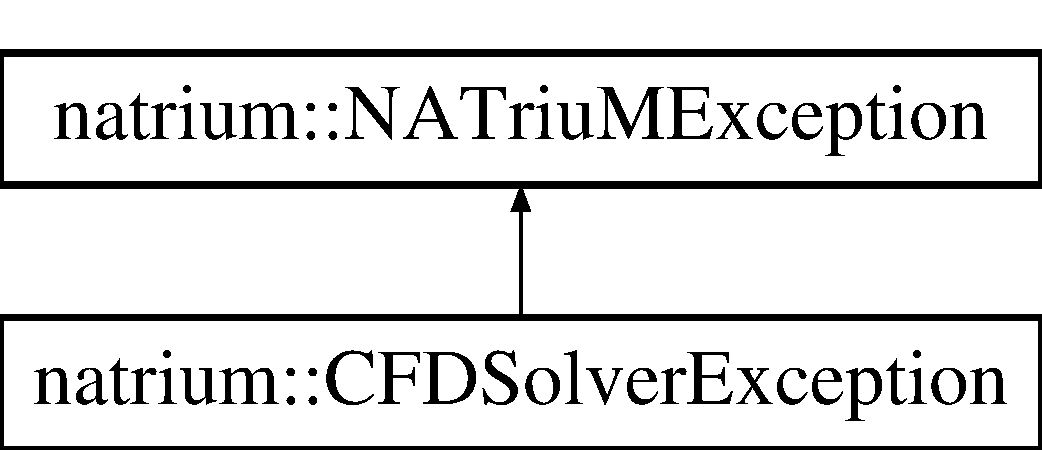
\includegraphics[height=2cm]{classnatrium_1_1CFDSolverException}
\end{center}
\end{figure}
\subsection*{Public Member Functions}
\begin{DoxyCompactItemize}
\item 
\hypertarget{classnatrium_1_1CFDSolverException_a1256570132b679d57fe046f648656051}{
{\bfseries CFDSolverException} (const char $\ast$msg)}
\label{classnatrium_1_1CFDSolverException_a1256570132b679d57fe046f648656051}

\item 
\hypertarget{classnatrium_1_1CFDSolverException_a1fc20604a6925cd3577fe3fa7c0f585e}{
{\bfseries CFDSolverException} (const string \&msg)}
\label{classnatrium_1_1CFDSolverException_a1fc20604a6925cd3577fe3fa7c0f585e}

\item 
\hypertarget{classnatrium_1_1CFDSolverException_ae1e5d3d088b808ab4c995d1209a86a1f}{
const char $\ast$ {\bfseries what} () const   throw ()}
\label{classnatrium_1_1CFDSolverException_ae1e5d3d088b808ab4c995d1209a86a1f}

\end{DoxyCompactItemize}


\subsection{Detailed Description}
Exception class for \hyperlink{classnatrium_1_1CFDSolver}{CFDSolver}. 

The documentation for this class was generated from the following file:\begin{DoxyCompactItemize}
\item 
/mnt/fdrive/akraem3m/workspace/NATriuM/src/library/natrium/solver/\hyperlink{CFDSolver_8h}{CFDSolver.h}\end{DoxyCompactItemize}

\hypertarget{classnatrium_1_1CollisionModel}{
\section{natrium::CollisionModel Class Reference}
\label{classnatrium_1_1CollisionModel}\index{natrium::CollisionModel@{natrium::CollisionModel}}
}


Abstract collision model. Required to have a common parent of all template specializations of Collision.  


{\ttfamily \#include $<$CollisionModel.h$>$}Inheritance diagram for natrium::CollisionModel::\begin{figure}[H]
\begin{center}
\leavevmode
\includegraphics[height=5cm]{classnatrium_1_1CollisionModel}
\end{center}
\end{figure}
\subsection*{Public Member Functions}
\begin{DoxyCompactItemize}
\item 
\hypertarget{classnatrium_1_1CollisionModel_a443734919886ea5880be3bba1257758d}{
{\bfseries CollisionModel} (const boost::shared\_\-ptr$<$ \hyperlink{classnatrium_1_1Stencil}{Stencil} $>$ stencil, ForceType force\_\-type=NO\_\-FORCING)}
\label{classnatrium_1_1CollisionModel_a443734919886ea5880be3bba1257758d}

\item 
\hypertarget{classnatrium_1_1CollisionModel_ac6c6d95633d62209a04528af86807025}{
virtual void {\bfseries collideAll} (\hyperlink{classnatrium_1_1DistributionFunctions}{DistributionFunctions} \&f, \hyperlink{namespacenatrium_a903d2b92917f582f2ff05f52160ab811}{distributed\_\-vector} \&densities, vector$<$ \hyperlink{namespacenatrium_a903d2b92917f582f2ff05f52160ab811}{distributed\_\-vector} $>$ \&velocities, const dealii::IndexSet \&locally\_\-owned\_\-dofs, bool inInitializationProcedure=false) const =0}
\label{classnatrium_1_1CollisionModel_ac6c6d95633d62209a04528af86807025}

\item 
\hypertarget{classnatrium_1_1CollisionModel_ab1ec1368662524bb87006f9038b4972d}{
virtual void {\bfseries setTimeStep} (double dt)}
\label{classnatrium_1_1CollisionModel_ab1ec1368662524bb87006f9038b4972d}

\item 
\hypertarget{classnatrium_1_1CollisionModel_ac10edd12e081a6eb48a36568f1bc1c0f}{
const boost::shared\_\-ptr$<$ \hyperlink{classnatrium_1_1Stencil}{Stencil} $>$ \& {\bfseries getStencil} () const }
\label{classnatrium_1_1CollisionModel_ac10edd12e081a6eb48a36568f1bc1c0f}

\item 
virtual double \hyperlink{classnatrium_1_1CollisionModel_ae1c879c87ac210a227a8e3da2d0ac385}{calculateDensity} (const vector$<$ double $>$ \&distributions) const 
\begin{DoxyCompactList}\small\item\em calculate macroscopic density \item\end{DoxyCompactList}\item 
virtual \hyperlink{namespacenatrium_a67c39077adc6634f8fa3762b8eef24c4}{numeric\_\-vector} \hyperlink{classnatrium_1_1CollisionModel_a90428f4c29916641de3de872803dde0f}{calculateVelocity} (const vector$<$ double $>$ \&distributions) const 
\begin{DoxyCompactList}\small\item\em calculate macroscopic velocity \item\end{DoxyCompactList}\item 
virtual void \hyperlink{classnatrium_1_1CollisionModel_a667f0e36da1bfb1c5102adb8f3afdcde}{calculateVelocity} (const vector$<$ double $>$ \&distributions, const double rho, \hyperlink{namespacenatrium_a67c39077adc6634f8fa3762b8eef24c4}{numeric\_\-vector} \&u) const 
\begin{DoxyCompactList}\small\item\em calculate macroscopic velocity; saves the double calculation of the density \item\end{DoxyCompactList}\item 
virtual double \hyperlink{classnatrium_1_1CollisionModel_a88b382d63da80e950bc58e8afad769a6}{getEquilibriumDistribution} (size\_\-t i, const \hyperlink{namespacenatrium_a67c39077adc6634f8fa3762b8eef24c4}{numeric\_\-vector} \&u, const double rho=1) const =0
\begin{DoxyCompactList}\small\item\em virtual function for the calculation of the equilibrium distribution \item\end{DoxyCompactList}\item 
virtual void \hyperlink{classnatrium_1_1CollisionModel_a296474961c4501bc23228be1d30ebf82}{getEquilibriumDistributions} (vector$<$ double $>$ \&feq, const \hyperlink{namespacenatrium_a67c39077adc6634f8fa3762b8eef24c4}{numeric\_\-vector} \&u, const double rho=1) const 
\begin{DoxyCompactList}\small\item\em function for the calculation of all equilibrium distributions \item\end{DoxyCompactList}\item 
\hypertarget{classnatrium_1_1CollisionModel_a44bababd58cae1fea650fe2bd86555b5}{
void {\bfseries setExternalForce} (const \hyperlink{classnatrium_1_1ConstantExternalForce}{ConstantExternalForce}$<$ 2 $>$ \&external\_\-force)}
\label{classnatrium_1_1CollisionModel_a44bababd58cae1fea650fe2bd86555b5}

\item 
\hypertarget{classnatrium_1_1CollisionModel_ae899a80c7dcfbbdb68dd6b4e4fff5a49}{
void {\bfseries setExternalForce} (const \hyperlink{classnatrium_1_1ConstantExternalForce}{ConstantExternalForce}$<$ 3 $>$ \&external\_\-force)}
\label{classnatrium_1_1CollisionModel_ae899a80c7dcfbbdb68dd6b4e4fff5a49}

\item 
\hypertarget{classnatrium_1_1CollisionModel_a6806e1494a2bbb03c27b146261af408b}{
ForceType {\bfseries getForceType} () const }
\label{classnatrium_1_1CollisionModel_a6806e1494a2bbb03c27b146261af408b}

\item 
\hypertarget{classnatrium_1_1CollisionModel_a366ae27de1bf045fd9bf0159e251054a}{
double {\bfseries getForceX} () const }
\label{classnatrium_1_1CollisionModel_a366ae27de1bf045fd9bf0159e251054a}

\item 
\hypertarget{classnatrium_1_1CollisionModel_a1282b42d5c270b9f031def96dbe15866}{
double {\bfseries getForceY} () const }
\label{classnatrium_1_1CollisionModel_a1282b42d5c270b9f031def96dbe15866}

\item 
\hypertarget{classnatrium_1_1CollisionModel_a60fa9f8c1614789027c553264524fb5e}{
double {\bfseries getForceZ} () const }
\label{classnatrium_1_1CollisionModel_a60fa9f8c1614789027c553264524fb5e}

\item 
\hypertarget{classnatrium_1_1CollisionModel_acff518f0353a95dfbf3ddeba2a7ed7f6}{
void {\bfseries setForceType} (ForceType forceType)}
\label{classnatrium_1_1CollisionModel_acff518f0353a95dfbf3ddeba2a7ed7f6}

\item 
\hypertarget{classnatrium_1_1CollisionModel_aa2a154a99039deb620501ef2e525089f}{
double {\bfseries getTimeStep} () const }
\label{classnatrium_1_1CollisionModel_aa2a154a99039deb620501ef2e525089f}

\item 
\hypertarget{classnatrium_1_1CollisionModel_a4ee445caf75fff704811e29fc46f431e}{
double {\bfseries getViscosity} () const }
\label{classnatrium_1_1CollisionModel_a4ee445caf75fff704811e29fc46f431e}

\item 
\hypertarget{classnatrium_1_1CollisionModel_a43cfd1efe035afb6f170b7b05c18113a}{
void {\bfseries setViscosity} (double viscosity)}
\label{classnatrium_1_1CollisionModel_a43cfd1efe035afb6f170b7b05c18113a}

\end{DoxyCompactItemize}


\subsection{Detailed Description}
Abstract collision model. Required to have a common parent of all template specializations of Collision. 

\subsection{Member Function Documentation}
\hypertarget{classnatrium_1_1CollisionModel_ae1c879c87ac210a227a8e3da2d0ac385}{
\index{natrium::CollisionModel@{natrium::CollisionModel}!calculateDensity@{calculateDensity}}
\index{calculateDensity@{calculateDensity}!natrium::CollisionModel@{natrium::CollisionModel}}
\subsubsection[{calculateDensity}]{\setlength{\rightskip}{0pt plus 5cm}virtual double natrium::CollisionModel::calculateDensity (const vector$<$ double $>$ \& {\em distributions}) const\hspace{0.3cm}{\ttfamily  \mbox{[}inline, virtual\mbox{]}}}}
\label{classnatrium_1_1CollisionModel_ae1c879c87ac210a227a8e3da2d0ac385}


calculate macroscopic density 
\begin{DoxyParams}{Parameters}
\item[\mbox{$\leftarrow$} {\em distributions}]particle distribution functions at a given point \end{DoxyParams}
\begin{DoxyReturn}{Returns}
macroscopic density (sum of all distributions) 
\end{DoxyReturn}


Reimplemented in \hyperlink{classnatrium_1_1BGKStandardTransformed_a58c4dc0c67ff4898c6555b614afc1ace}{natrium::BGKStandardTransformed}.\hypertarget{classnatrium_1_1CollisionModel_a667f0e36da1bfb1c5102adb8f3afdcde}{
\index{natrium::CollisionModel@{natrium::CollisionModel}!calculateVelocity@{calculateVelocity}}
\index{calculateVelocity@{calculateVelocity}!natrium::CollisionModel@{natrium::CollisionModel}}
\subsubsection[{calculateVelocity}]{\setlength{\rightskip}{0pt plus 5cm}virtual void natrium::CollisionModel::calculateVelocity (const vector$<$ double $>$ \& {\em distributions}, \/  const double {\em rho}, \/  {\bf numeric\_\-vector} \& {\em u}) const\hspace{0.3cm}{\ttfamily  \mbox{[}inline, virtual\mbox{]}}}}
\label{classnatrium_1_1CollisionModel_a667f0e36da1bfb1c5102adb8f3afdcde}


calculate macroscopic velocity; saves the double calculation of the density \begin{DoxyNote}{Note}
more efficient 
\end{DoxyNote}

\begin{DoxyParams}{Parameters}
\item[\mbox{$\leftarrow$} {\em distributions}]particle distribution functions at a given point \item[\mbox{$\leftarrow$} {\em rho}]macroscopic density \item[\mbox{$\rightarrow$} {\em u}]macroscopic velocity \end{DoxyParams}
\hypertarget{classnatrium_1_1CollisionModel_a90428f4c29916641de3de872803dde0f}{
\index{natrium::CollisionModel@{natrium::CollisionModel}!calculateVelocity@{calculateVelocity}}
\index{calculateVelocity@{calculateVelocity}!natrium::CollisionModel@{natrium::CollisionModel}}
\subsubsection[{calculateVelocity}]{\setlength{\rightskip}{0pt plus 5cm}virtual {\bf numeric\_\-vector} natrium::CollisionModel::calculateVelocity (const vector$<$ double $>$ \& {\em distributions}) const\hspace{0.3cm}{\ttfamily  \mbox{[}inline, virtual\mbox{]}}}}
\label{classnatrium_1_1CollisionModel_a90428f4c29916641de3de872803dde0f}


calculate macroscopic velocity 
\begin{DoxyParams}{Parameters}
\item[\mbox{$\leftarrow$} {\em distributions}]particle distribution functions at a given point \end{DoxyParams}
\begin{DoxyReturn}{Returns}
macroscopic velocity 
\end{DoxyReturn}
\hypertarget{classnatrium_1_1CollisionModel_a88b382d63da80e950bc58e8afad769a6}{
\index{natrium::CollisionModel@{natrium::CollisionModel}!getEquilibriumDistribution@{getEquilibriumDistribution}}
\index{getEquilibriumDistribution@{getEquilibriumDistribution}!natrium::CollisionModel@{natrium::CollisionModel}}
\subsubsection[{getEquilibriumDistribution}]{\setlength{\rightskip}{0pt plus 5cm}virtual double natrium::CollisionModel::getEquilibriumDistribution (size\_\-t {\em i}, \/  const {\bf numeric\_\-vector} \& {\em u}, \/  const double {\em rho} = {\ttfamily 1}) const\hspace{0.3cm}{\ttfamily  \mbox{[}pure virtual\mbox{]}}}}
\label{classnatrium_1_1CollisionModel_a88b382d63da80e950bc58e8afad769a6}


virtual function for the calculation of the equilibrium distribution 
\begin{DoxyParams}{Parameters}
\item[{\em i}]index of the direction \item[{\em u}]macroscopic velocity \item[{\em rho}]macroscopic density \end{DoxyParams}
\begin{DoxyReturn}{Returns}
value of the equilibrium distribution 
\end{DoxyReturn}
\begin{DoxyNote}{Note}
The calculation can surely be done more efficiently by passing different arguments, e.g. u$\ast$u or u/(c$^\wedge$2) 
\end{DoxyNote}


Implemented in \hyperlink{classnatrium_1_1BGKIncompressible_a26dd8954261b04f8383ca9d37f5ac8c0}{natrium::BGKIncompressible}, \hyperlink{classnatrium_1_1BGKMultistep_a034cd475974bcce0db64e52245efd91d}{natrium::BGKMultistep}, \hyperlink{classnatrium_1_1BGKPseudopotential_a366ccd417ca4ad5fa37ce0572e0d6fe4}{natrium::BGKPseudopotential$<$ dim $>$}, \hyperlink{classnatrium_1_1BGKStandard_a3d45ef2fe5536bf14914f99297477754}{natrium::BGKStandard}, \hyperlink{classnatrium_1_1BGKStandardTransformed_a870465cc026f92c8ffba899af6f95634}{natrium::BGKStandardTransformed}, \hyperlink{classnatrium_1_1BGKSteadyState_ad99d9159cc14b5897bea7f145c3b39ca}{natrium::BGKSteadyState}, \hyperlink{classnatrium_1_1KBCStandard_a1dac2deaafb93027bf168887dd2e002d}{natrium::KBCStandard}, and \hyperlink{classnatrium_1_1MRT_a3f96915f9f67680f4a1d7b952e70be55}{natrium::MRT}.\hypertarget{classnatrium_1_1CollisionModel_a296474961c4501bc23228be1d30ebf82}{
\index{natrium::CollisionModel@{natrium::CollisionModel}!getEquilibriumDistributions@{getEquilibriumDistributions}}
\index{getEquilibriumDistributions@{getEquilibriumDistributions}!natrium::CollisionModel@{natrium::CollisionModel}}
\subsubsection[{getEquilibriumDistributions}]{\setlength{\rightskip}{0pt plus 5cm}void natrium::CollisionModel::getEquilibriumDistributions (vector$<$ double $>$ \& {\em feq}, \/  const {\bf numeric\_\-vector} \& {\em u}, \/  const double {\em rho} = {\ttfamily 1}) const\hspace{0.3cm}{\ttfamily  \mbox{[}virtual\mbox{]}}}}
\label{classnatrium_1_1CollisionModel_a296474961c4501bc23228be1d30ebf82}


function for the calculation of all equilibrium distributions 
\begin{DoxyParams}{Parameters}
\item[\mbox{$\rightarrow$} {\em feq}]vector of all equality distributions, must have size Q \item[\mbox{$\leftarrow$} {\em u}]macroscopic velocity \item[\mbox{$\leftarrow$} {\em rho}]macroscopic density \end{DoxyParams}
\begin{DoxyNote}{Note}
The calculation can surely be done more efficiently by passing different arguments, e.g. u$\ast$u or u/(c$^\wedge$2) 
\end{DoxyNote}


The documentation for this class was generated from the following files:\begin{DoxyCompactItemize}
\item 
/mnt/fdrive/akraem3m/workspace/NATriuM/src/library/natrium/collision/\hyperlink{CollisionModel_8h}{CollisionModel.h}\item 
/mnt/fdrive/akraem3m/workspace/NATriuM/src/library/natrium/collision/\hyperlink{CollisionModel_8cpp}{CollisionModel.cpp}\end{DoxyCompactItemize}

\hypertarget{classnatrium_1_1ConfigurationException}{\section{natrium\-:\-:Configuration\-Exception Class Reference}
\label{classnatrium_1_1ConfigurationException}\index{natrium\-::\-Configuration\-Exception@{natrium\-::\-Configuration\-Exception}}
}


Exception class for \hyperlink{classnatrium_1_1CFDSolver}{C\-F\-D\-Solver}.  




{\ttfamily \#include $<$Solver\-Configuration.\-h$>$}

Inheritance diagram for natrium\-:\-:Configuration\-Exception\-:\begin{figure}[H]
\begin{center}
\leavevmode
\includegraphics[height=2.000000cm]{classnatrium_1_1ConfigurationException}
\end{center}
\end{figure}
\subsection*{Public Member Functions}
\begin{DoxyCompactItemize}
\item 
\hypertarget{classnatrium_1_1ConfigurationException_ac9248a6224570c873784f201ef9ae34f}{{\bfseries Configuration\-Exception} (const char $\ast$msg)}\label{classnatrium_1_1ConfigurationException_ac9248a6224570c873784f201ef9ae34f}

\item 
\hypertarget{classnatrium_1_1ConfigurationException_a9f622f88d955e5c5e01719b7fcb273a6}{{\bfseries Configuration\-Exception} (const string \&msg)}\label{classnatrium_1_1ConfigurationException_a9f622f88d955e5c5e01719b7fcb273a6}

\item 
\hypertarget{classnatrium_1_1ConfigurationException_a48c72bd9bbae81e098a1f214899b3de6}{const char $\ast$ {\bfseries what} () const   throw ()}\label{classnatrium_1_1ConfigurationException_a48c72bd9bbae81e098a1f214899b3de6}

\end{DoxyCompactItemize}


\subsection{Detailed Description}
Exception class for \hyperlink{classnatrium_1_1CFDSolver}{C\-F\-D\-Solver}. 

The documentation for this class was generated from the following file\-:\begin{DoxyCompactItemize}
\item 
/home/kraemer/eclipse\-\_\-workspace/\-N\-A\-Triu\-M/src/natrium/solver/\hyperlink{SolverConfiguration_8h}{Solver\-Configuration.\-h}\end{DoxyCompactItemize}

\hypertarget{classnatrium_1_1CouetteFlow2D}{\section{natrium\-:\-:Couette\-Flow2\-D Class Reference}
\label{classnatrium_1_1CouetteFlow2D}\index{natrium\-::\-Couette\-Flow2\-D@{natrium\-::\-Couette\-Flow2\-D}}
}


Description of a simple Couette Flow (regular channel flow in square domain). The domain is \mbox{[}0,1\mbox{]}$^\wedge$2. The top plate is moved with constant velocity. The domain consists of 8 x 8 = 64 Elements (contrast to Min and Lee, who have 6 x 6).  




{\ttfamily \#include $<$Couette\-Flow2\-D.\-h$>$}

Inheritance diagram for natrium\-:\-:Couette\-Flow2\-D\-:\begin{figure}[H]
\begin{center}
\leavevmode
\includegraphics[height=3.000000cm]{classnatrium_1_1CouetteFlow2D}
\end{center}
\end{figure}
\subsection*{Public Member Functions}
\begin{DoxyCompactItemize}
\item 
\hyperlink{classnatrium_1_1CouetteFlow2D_ac5abfdca75a910fb11cad175942de50f}{Couette\-Flow2\-D} (double viscosity, double top\-Plate\-Velocity, size\-\_\-t refinement\-Level, double L=1.\-0, double start\-Time=0.\-0)
\begin{DoxyCompactList}\small\item\em constructor \end{DoxyCompactList}\item 
\hypertarget{classnatrium_1_1CouetteFlow2D_a97b61b0f71dc653427ba3db46e185873}{virtual \hyperlink{classnatrium_1_1CouetteFlow2D_a97b61b0f71dc653427ba3db46e185873}{$\sim$\-Couette\-Flow2\-D} ()}\label{classnatrium_1_1CouetteFlow2D_a97b61b0f71dc653427ba3db46e185873}

\begin{DoxyCompactList}\small\item\em destructor \end{DoxyCompactList}\item 
\hypertarget{classnatrium_1_1CouetteFlow2D_a3953d81acbab33424dfc4135930253df}{virtual void \hyperlink{classnatrium_1_1CouetteFlow2D_a3953d81acbab33424dfc4135930253df}{get\-Analytic\-Velocity} (const dealii\-::\-Point$<$ 2 $>$ \&x, double t, dealii\-::\-Point$<$ 2 $>$ \&velocity) const }\label{classnatrium_1_1CouetteFlow2D_a3953d81acbab33424dfc4135930253df}

\begin{DoxyCompactList}\small\item\em analytic solution of the Taylor-\/\-Green vortex \end{DoxyCompactList}\item 
\hypertarget{classnatrium_1_1CouetteFlow2D_a74429d98c455a0c06430a665505d8375}{virtual double {\bfseries get\-Characteristic\-Velocity} () const }\label{classnatrium_1_1CouetteFlow2D_a74429d98c455a0c06430a665505d8375}

\end{DoxyCompactItemize}


\subsection{Detailed Description}
Description of a simple Couette Flow (regular channel flow in square domain). The domain is \mbox{[}0,1\mbox{]}$^\wedge$2. The top plate is moved with constant velocity. The domain consists of 8 x 8 = 64 Elements (contrast to Min and Lee, who have 6 x 6). 

\begin{DoxyNote}{Note}
The analytic solution is obtained by a formula stated in Min and Lee (2011). 
\end{DoxyNote}


\subsection{Constructor \& Destructor Documentation}
\hypertarget{classnatrium_1_1CouetteFlow2D_ac5abfdca75a910fb11cad175942de50f}{\index{natrium\-::\-Couette\-Flow2\-D@{natrium\-::\-Couette\-Flow2\-D}!Couette\-Flow2\-D@{Couette\-Flow2\-D}}
\index{Couette\-Flow2\-D@{Couette\-Flow2\-D}!natrium::CouetteFlow2D@{natrium\-::\-Couette\-Flow2\-D}}
\subsubsection[{Couette\-Flow2\-D}]{\setlength{\rightskip}{0pt plus 5cm}natrium\-::\-Couette\-Flow2\-D\-::\-Couette\-Flow2\-D (
\begin{DoxyParamCaption}
\item[{double}]{viscosity, }
\item[{double}]{top\-Plate\-Velocity, }
\item[{size\-\_\-t}]{refinement\-Level, }
\item[{double}]{L = {\ttfamily 1.0}, }
\item[{double}]{start\-Time = {\ttfamily 0.0}}
\end{DoxyParamCaption}
)}}\label{classnatrium_1_1CouetteFlow2D_ac5abfdca75a910fb11cad175942de50f}


constructor 

apply boundary values 

The documentation for this class was generated from the following files\-:\begin{DoxyCompactItemize}
\item 
/home/kraemer/eclipse\-\_\-workspace/\-N\-A\-Triu\-M/src/examples/step-\/2/\hyperlink{CouetteFlow2D_8h}{Couette\-Flow2\-D.\-h}\item 
/home/kraemer/eclipse\-\_\-workspace/\-N\-A\-Triu\-M/src/examples/step-\/2/\hyperlink{CouetteFlow2D_8cpp}{Couette\-Flow2\-D.\-cpp}\end{DoxyCompactItemize}

\hypertarget{classnatrium_1_1D2Q9IncompressibleModel}{\section{natrium\-:\-:\-D2\-Q9\-Incompressible\-Model \-Class \-Reference}
\label{classnatrium_1_1D2Q9IncompressibleModel}\index{natrium\-::\-D2\-Q9\-Incompressible\-Model@{natrium\-::\-D2\-Q9\-Incompressible\-Model}}
}


\-D2\-Q9 model description for incompressible flow.  




{\ttfamily \#include $<$\-D2\-Q9\-Incompressible\-Model.\-h$>$}

\-Inheritance diagram for natrium\-:\-:\-D2\-Q9\-Incompressible\-Model\-:\begin{figure}[H]
\begin{center}
\leavevmode
\includegraphics[height=3.000000cm]{classnatrium_1_1D2Q9IncompressibleModel}
\end{center}
\end{figure}
\subsection*{\-Public \-Member \-Functions}
\begin{DoxyCompactItemize}
\item 
\hypertarget{classnatrium_1_1D2Q9IncompressibleModel_a50cce01cb87eb811013079d73c4baaf0}{\hyperlink{classnatrium_1_1D2Q9IncompressibleModel_a50cce01cb87eb811013079d73c4baaf0}{\-D2\-Q9\-Incompressible\-Model} ()}\label{classnatrium_1_1D2Q9IncompressibleModel_a50cce01cb87eb811013079d73c4baaf0}

\begin{DoxyCompactList}\small\item\em constructor \end{DoxyCompactList}\item 
virtual \hyperlink{classnatrium_1_1D2Q9IncompressibleModel_a6e757941f7ca2c5a6148893147211724}{$\sim$\-D2\-Q9\-Incompressible\-Model} ()
\begin{DoxyCompactList}\small\item\em destructor \end{DoxyCompactList}\item 
virtual float\-\_\-t \hyperlink{classnatrium_1_1D2Q9IncompressibleModel_a437bce6e0d6f35ca3ff2df4bbe650043}{get\-Equilibrium\-Distribution} (size\-\_\-t i, const numeric\-\_\-vector \&u, const float\-\_\-t rho=1) const 
\begin{DoxyCompactList}\small\item\em function for the calculation of the equilibrium distribution in the incompressible \-D2\-Q9 model \end{DoxyCompactList}\end{DoxyCompactItemize}


\subsection{\-Detailed \-Description}
\-D2\-Q9 model description for incompressible flow. 

\subsection{\-Constructor \& \-Destructor \-Documentation}
\hypertarget{classnatrium_1_1D2Q9IncompressibleModel_a6e757941f7ca2c5a6148893147211724}{\index{natrium\-::\-D2\-Q9\-Incompressible\-Model@{natrium\-::\-D2\-Q9\-Incompressible\-Model}!$\sim$\-D2\-Q9\-Incompressible\-Model@{$\sim$\-D2\-Q9\-Incompressible\-Model}}
\index{$\sim$\-D2\-Q9\-Incompressible\-Model@{$\sim$\-D2\-Q9\-Incompressible\-Model}!natrium::D2Q9IncompressibleModel@{natrium\-::\-D2\-Q9\-Incompressible\-Model}}
\subsubsection[{$\sim$\-D2\-Q9\-Incompressible\-Model}]{\setlength{\rightskip}{0pt plus 5cm}{\bf natrium\-::\-D2\-Q9\-Incompressible\-Model\-::$\sim$\-D2\-Q9\-Incompressible\-Model} (
\begin{DoxyParamCaption}
{}
\end{DoxyParamCaption}
)\hspace{0.3cm}{\ttfamily  \mbox{[}virtual\mbox{]}}}}\label{classnatrium_1_1D2Q9IncompressibleModel_a6e757941f7ca2c5a6148893147211724}


destructor 

constructor 

\subsection{\-Member \-Function \-Documentation}
\hypertarget{classnatrium_1_1D2Q9IncompressibleModel_a437bce6e0d6f35ca3ff2df4bbe650043}{\index{natrium\-::\-D2\-Q9\-Incompressible\-Model@{natrium\-::\-D2\-Q9\-Incompressible\-Model}!get\-Equilibrium\-Distribution@{get\-Equilibrium\-Distribution}}
\index{get\-Equilibrium\-Distribution@{get\-Equilibrium\-Distribution}!natrium::D2Q9IncompressibleModel@{natrium\-::\-D2\-Q9\-Incompressible\-Model}}
\subsubsection[{get\-Equilibrium\-Distribution}]{\setlength{\rightskip}{0pt plus 5cm}float\-\_\-t {\bf natrium\-::\-D2\-Q9\-Incompressible\-Model\-::get\-Equilibrium\-Distribution} (
\begin{DoxyParamCaption}
\item[{size\-\_\-t}]{i, }
\item[{const numeric\-\_\-vector \&}]{u, }
\item[{const float\-\_\-t}]{rho = {\ttfamily 1}}
\end{DoxyParamCaption}
) const\hspace{0.3cm}{\ttfamily  \mbox{[}virtual\mbox{]}}}}\label{classnatrium_1_1D2Q9IncompressibleModel_a437bce6e0d6f35ca3ff2df4bbe650043}


function for the calculation of the equilibrium distribution in the incompressible \-D2\-Q9 model 

destructor


\begin{DoxyParams}{\-Parameters}
{\em i} & index of the direction \\
\hline
{\em u} & macroscopic velocity \\
\hline
{\em rho} & macroscopic density \\
\hline
\end{DoxyParams}
\begin{DoxyReturn}{\-Returns}
value of the equilibrium distribution 
\end{DoxyReturn}
\begin{DoxyNote}{\-Note}
\-The calculation can surely be done more efficiently by passing different arguments, e.\-g. u$\ast$u or u/(c$^\wedge$2)
\end{DoxyNote}
get\-Equilibrium\-Distribution 

\-Implements \hyperlink{classnatrium_1_1BoltzmannModel_ac5615f43cd5c03c881734d4826ce31be}{natrium\-::\-Boltzmann\-Model}.



\-The documentation for this class was generated from the following files\-:\begin{DoxyCompactItemize}
\item 
/home/kraemer/eclipse\-\_\-workspace/\-N\-A\-Triu\-M/src/boltzmannmodels/\-D2\-Q9\-Incompressible\-Model.\-h\item 
/home/kraemer/eclipse\-\_\-workspace/\-N\-A\-Triu\-M/src/boltzmannmodels/\-D2\-Q9\-Incompressible\-Model.\-cpp\end{DoxyCompactItemize}

\hypertarget{classnatrium_1_1D2Q9Model}{\section{natrium\-:\-:D2\-Q9\-Model Class Reference}
\label{classnatrium_1_1D2Q9Model}\index{natrium\-::\-D2\-Q9\-Model@{natrium\-::\-D2\-Q9\-Model}}
}


D2\-Q9 Model.  




{\ttfamily \#include $<$D2\-Q9\-Model.\-h$>$}

Inheritance diagram for natrium\-:\-:D2\-Q9\-Model\-:\begin{figure}[H]
\begin{center}
\leavevmode
\includegraphics[height=3.000000cm]{classnatrium_1_1D2Q9Model}
\end{center}
\end{figure}
\subsection*{Public Member Functions}
\begin{DoxyCompactItemize}
\item 
\hypertarget{classnatrium_1_1D2Q9Model_af498c14d311e9172d96b5d962ccc5202}{\hyperlink{classnatrium_1_1D2Q9Model_af498c14d311e9172d96b5d962ccc5202}{D2\-Q9\-Model} (double scaling)}\label{classnatrium_1_1D2Q9Model_af498c14d311e9172d96b5d962ccc5202}

\begin{DoxyCompactList}\small\item\em constructor \end{DoxyCompactList}\item 
\hypertarget{classnatrium_1_1D2Q9Model_aec7d8c160f430e14fbede9ecda368797}{virtual \hyperlink{classnatrium_1_1D2Q9Model_aec7d8c160f430e14fbede9ecda368797}{$\sim$\-D2\-Q9\-Model} ()}\label{classnatrium_1_1D2Q9Model_aec7d8c160f430e14fbede9ecda368797}

\begin{DoxyCompactList}\small\item\em destructor \end{DoxyCompactList}\item 
\hypertarget{classnatrium_1_1D2Q9Model_ac9b53eb73e84ecd13afcf9f3a0b0e195}{virtual double {\bfseries get\-Speed\-Of\-Sound} () const }\label{classnatrium_1_1D2Q9Model_ac9b53eb73e84ecd13afcf9f3a0b0e195}

\item 
\hypertarget{classnatrium_1_1D2Q9Model_aa83e54b682ec7081c298324ee9688a8e}{virtual double {\bfseries get\-Speed\-Of\-Sound\-Square} () const }\label{classnatrium_1_1D2Q9Model_aa83e54b682ec7081c298324ee9688a8e}

\item 
\hypertarget{classnatrium_1_1D2Q9Model_ae29e3df458e24802467ca9c2209cc0ca}{virtual size\-\_\-t {\bfseries get\-Index\-Of\-Opposite\-Direction} (size\-\_\-t index) const }\label{classnatrium_1_1D2Q9Model_ae29e3df458e24802467ca9c2209cc0ca}

\item 
\hypertarget{classnatrium_1_1D2Q9Model_a3e853f0d03f85f2c6eea3bd799c3b040}{virtual double {\bfseries get\-Max\-Particle\-Velocity\-Magnitude} () const }\label{classnatrium_1_1D2Q9Model_a3e853f0d03f85f2c6eea3bd799c3b040}

\item 
\hypertarget{classnatrium_1_1D2Q9Model_a4a72be5ee163c19b9e2a0210ff54cd57}{const double {\bfseries get\-Scaling} () const }\label{classnatrium_1_1D2Q9Model_a4a72be5ee163c19b9e2a0210ff54cd57}

\end{DoxyCompactItemize}
\subsection*{Static Public Attributes}
\begin{DoxyCompactItemize}
\item 
\hypertarget{classnatrium_1_1D2Q9Model_a81532a1067ba5f280698a1a84711ede5}{static const size\-\_\-t \hyperlink{classnatrium_1_1D2Q9Model_a81532a1067ba5f280698a1a84711ede5}{D} = 2}\label{classnatrium_1_1D2Q9Model_a81532a1067ba5f280698a1a84711ede5}

\begin{DoxyCompactList}\small\item\em D. \end{DoxyCompactList}\item 
\hypertarget{classnatrium_1_1D2Q9Model_ad3d102dfb9c8ad7b56a8f82c3f4286f6}{static const size\-\_\-t \hyperlink{classnatrium_1_1D2Q9Model_ad3d102dfb9c8ad7b56a8f82c3f4286f6}{Q} = 9}\label{classnatrium_1_1D2Q9Model_ad3d102dfb9c8ad7b56a8f82c3f4286f6}

\begin{DoxyCompactList}\small\item\em Q. \end{DoxyCompactList}\end{DoxyCompactItemize}
\subsection*{Protected Attributes}
\begin{DoxyCompactItemize}
\item 
\hypertarget{classnatrium_1_1D2Q9Model_ab212c0c04921591f16c1970d93878cf9}{const double \hyperlink{classnatrium_1_1D2Q9Model_ab212c0c04921591f16c1970d93878cf9}{m\-\_\-speed\-Of\-Sound}}\label{classnatrium_1_1D2Q9Model_ab212c0c04921591f16c1970d93878cf9}

\begin{DoxyCompactList}\small\item\em speed of sound \end{DoxyCompactList}\item 
\hypertarget{classnatrium_1_1D2Q9Model_afa28316438de5055d51674d89a0075ba}{const double \hyperlink{classnatrium_1_1D2Q9Model_afa28316438de5055d51674d89a0075ba}{m\-\_\-speed\-Of\-Sound\-Square}}\label{classnatrium_1_1D2Q9Model_afa28316438de5055d51674d89a0075ba}

\begin{DoxyCompactList}\small\item\em (speed of sound)$^\wedge$2 \end{DoxyCompactList}\item 
\hypertarget{classnatrium_1_1D2Q9Model_ab0aa145ad44fe849371f8bda592eadf2}{const double \hyperlink{classnatrium_1_1D2Q9Model_ab0aa145ad44fe849371f8bda592eadf2}{m\-\_\-scaling}}\label{classnatrium_1_1D2Q9Model_ab0aa145ad44fe849371f8bda592eadf2}

\begin{DoxyCompactList}\small\item\em scaling of the stencil \end{DoxyCompactList}\end{DoxyCompactItemize}


\subsection{Detailed Description}
D2\-Q9 Model. 

The documentation for this class was generated from the following files\-:\begin{DoxyCompactItemize}
\item 
/home/kraemer/eclipse\-\_\-workspace/\-N\-A\-Triu\-M/src/natrium/boltzmannmodels/\hyperlink{D2Q9Model_8h}{D2\-Q9\-Model.\-h}\item 
/home/kraemer/eclipse\-\_\-workspace/\-N\-A\-Triu\-M/src/natrium/boltzmannmodels/\hyperlink{D2Q9Model_8cpp}{D2\-Q9\-Model.\-cpp}\end{DoxyCompactItemize}

\hypertarget{classnatrium_1_1ExponentialTimeIntegrator}{\section{natrium\-:\-:Exponential\-Time\-Integrator Class Reference}
\label{classnatrium_1_1ExponentialTimeIntegrator}\index{natrium\-::\-Exponential\-Time\-Integrator@{natrium\-::\-Exponential\-Time\-Integrator}}
}


Exponential time integration scheme for the solution of f' = L$\ast$f, as used in Uga etal. (2012) Spectral-\/element discontinuous Galerkin lattice Boltzmann simulation of flow past two cylinders in tandem with an exponential time integrator, C\-M\-W\-A 65 pp. 239-\/251.  




{\ttfamily \#include $<$Exponential\-Time\-Integrator.\-h$>$}

\subsection*{Public Member Functions}
\begin{DoxyCompactItemize}
\item 
\hypertarget{classnatrium_1_1ExponentialTimeIntegrator_a91472d03faddf0e2166fb5d77e6cb062}{\hyperlink{classnatrium_1_1ExponentialTimeIntegrator_a91472d03faddf0e2166fb5d77e6cb062}{Exponential\-Time\-Integrator} ()}\label{classnatrium_1_1ExponentialTimeIntegrator_a91472d03faddf0e2166fb5d77e6cb062}

\begin{DoxyCompactList}\small\item\em constructor \end{DoxyCompactList}\item 
\hypertarget{classnatrium_1_1ExponentialTimeIntegrator_a7114f9845feb896b3129492de36a60b3}{virtual \hyperlink{classnatrium_1_1ExponentialTimeIntegrator_a7114f9845feb896b3129492de36a60b3}{$\sim$\-Exponential\-Time\-Integrator} ()}\label{classnatrium_1_1ExponentialTimeIntegrator_a7114f9845feb896b3129492de36a60b3}

\begin{DoxyCompactList}\small\item\em destructor \end{DoxyCompactList}\end{DoxyCompactItemize}


\subsection{Detailed Description}
Exponential time integration scheme for the solution of f' = L$\ast$f, as used in Uga etal. (2012) Spectral-\/element discontinuous Galerkin lattice Boltzmann simulation of flow past two cylinders in tandem with an exponential time integrator, C\-M\-W\-A 65 pp. 239-\/251. 

The documentation for this class was generated from the following files\-:\begin{DoxyCompactItemize}
\item 
/home/kraemer/eclipse\-\_\-workspace/\-N\-A\-Triu\-M/src/natrium/timeintegration/\hyperlink{ExponentialTimeIntegrator_8h}{Exponential\-Time\-Integrator.\-h}\item 
/home/kraemer/eclipse\-\_\-workspace/\-N\-A\-Triu\-M/src/natrium/timeintegration/\hyperlink{ExponentialTimeIntegrator_8cpp}{Exponential\-Time\-Integrator.\-cpp}\end{DoxyCompactItemize}

\hypertarget{classnatrium_1_1Logging}{\section{natrium\-:\-:Logging Class Reference}
\label{classnatrium_1_1Logging}\index{natrium\-::\-Logging@{natrium\-::\-Logging}}
}


this class is responsible for output streams to the command line and log file  




{\ttfamily \#include $<$Logging.\-h$>$}

Inheritance diagram for natrium\-:\-:Logging\-:\begin{figure}[H]
\begin{center}
\leavevmode
\includegraphics[height=2.000000cm]{classnatrium_1_1Logging}
\end{center}
\end{figure}
\subsection*{Public Member Functions}
\begin{DoxyCompactItemize}
\item 
\hypertarget{classnatrium_1_1Logging_a255455c6e8a6c109a8e7e905bdd57ea3}{\hyperlink{classnatrium_1_1Logging_a255455c6e8a6c109a8e7e905bdd57ea3}{Logging} ()}\label{classnatrium_1_1Logging_a255455c6e8a6c109a8e7e905bdd57ea3}

\begin{DoxyCompactList}\small\item\em constructor \end{DoxyCompactList}\item 
\hypertarget{classnatrium_1_1Logging_a2bfeafec90e8b3fdceddc2866fda6e3d}{\hyperlink{classnatrium_1_1Logging}{Logging} \& \hyperlink{classnatrium_1_1Logging_a2bfeafec90e8b3fdceddc2866fda6e3d}{operator()} (Log\-Level level)}\label{classnatrium_1_1Logging_a2bfeafec90e8b3fdceddc2866fda6e3d}

\begin{DoxyCompactList}\small\item\em set log level for command line output \end{DoxyCompactList}\item 
\hypertarget{classnatrium_1_1Logging_a6dc3bdfa386b24a031578f9293a24403}{void \hyperlink{classnatrium_1_1Logging_a6dc3bdfa386b24a031578f9293a24403}{set\-Log\-File} (string log\-File)}\label{classnatrium_1_1Logging_a6dc3bdfa386b24a031578f9293a24403}

\begin{DoxyCompactList}\small\item\em set log file \end{DoxyCompactList}\item 
\hypertarget{classnatrium_1_1Logging_aae32db6189a7c963323a869821bb26d9}{void \hyperlink{classnatrium_1_1Logging_aae32db6189a7c963323a869821bb26d9}{unset\-Log\-File} (string log\-File)}\label{classnatrium_1_1Logging_aae32db6189a7c963323a869821bb26d9}

\begin{DoxyCompactList}\small\item\em detach log file \end{DoxyCompactList}\item 
\hypertarget{classnatrium_1_1Logging_a1bfdfbdfdf8a69e9aa9d6ffa78cb3d45}{Log\-Level \hyperlink{classnatrium_1_1Logging_a1bfdfbdfdf8a69e9aa9d6ffa78cb3d45}{set\-Console\-Level} (Log\-Level level)}\label{classnatrium_1_1Logging_a1bfdfbdfdf8a69e9aa9d6ffa78cb3d45}

\begin{DoxyCompactList}\small\item\em set the level of console output \end{DoxyCompactList}\item 
\hypertarget{classnatrium_1_1Logging_a21852bc69b5ff32f5ec5241a810ab8d5}{Log\-Level \hyperlink{classnatrium_1_1Logging_a21852bc69b5ff32f5ec5241a810ab8d5}{set\-File\-Level} (Log\-Level level)}\label{classnatrium_1_1Logging_a21852bc69b5ff32f5ec5241a810ab8d5}

\begin{DoxyCompactList}\small\item\em set the level of file output \end{DoxyCompactList}\end{DoxyCompactItemize}
\subsection*{Friends}
\begin{DoxyCompactItemize}
\item 
\hyperlink{classnatrium_1_1Logging}{Logging} \& \hyperlink{classnatrium_1_1Logging_a913b816565b3ede4c25b89d25ca5148d}{L\-O\-G} (Log\-Level level)
\begin{DoxyCompactList}\small\item\em friend function; can be used like \char`\"{}\-L\-O\-G(\-E\-R\-R\-O\-R) $<$$<$ ...;\char`\"{}, to write output to the log file and command line \end{DoxyCompactList}\item 
\hypertarget{classnatrium_1_1Logging_a9339ce5458ee8cadf69734faf310c21b}{\hyperlink{classnatrium_1_1Logging}{Logging} \& \hyperlink{classnatrium_1_1Logging_a9339ce5458ee8cadf69734faf310c21b}{L\-O\-G\-G\-E\-R} ()}\label{classnatrium_1_1Logging_a9339ce5458ee8cadf69734faf310c21b}

\begin{DoxyCompactList}\small\item\em friend function; is used to access the default logging instance; e.\-g. \hyperlink{classnatrium_1_1Logging_a9339ce5458ee8cadf69734faf310c21b}{L\-O\-G\-G\-E\-R()}.set\-Log\-File(...) \end{DoxyCompactList}\end{DoxyCompactItemize}


\subsection{Detailed Description}
this class is responsible for output streams to the command line and log file 

\begin{DoxyNote}{Note}
As normally there is only one ouput stream needed, this class provides the possibily to access the default logging instance from everywhere. The friend functions L\-O\-G and L\-O\-G\-G\-E\-R are used as a wrapper around the private, but static, m\-\_\-\-L\-O\-G\-G\-E\-R. When m\-\_\-\-L\-O\-G\-G\-E\-R does not exists, it is created by L\-O\-G or L\-O\-G\-G\-E\-R. 
\end{DoxyNote}


\subsection{Friends And Related Function Documentation}
\hypertarget{classnatrium_1_1Logging_a913b816565b3ede4c25b89d25ca5148d}{\index{natrium\-::\-Logging@{natrium\-::\-Logging}!L\-O\-G@{L\-O\-G}}
\index{L\-O\-G@{L\-O\-G}!natrium::Logging@{natrium\-::\-Logging}}
\subsubsection[{L\-O\-G}]{\setlength{\rightskip}{0pt plus 5cm}{\bf Logging}\& L\-O\-G (
\begin{DoxyParamCaption}
\item[{Log\-Level}]{level}
\end{DoxyParamCaption}
)\hspace{0.3cm}{\ttfamily [friend]}}}\label{classnatrium_1_1Logging_a913b816565b3ede4c25b89d25ca5148d}


friend function; can be used like \char`\"{}\-L\-O\-G(\-E\-R\-R\-O\-R) $<$$<$ ...;\char`\"{}, to write output to the log file and command line 

\begin{DoxyNote}{Note}
accesses the default logstream Logging\-::m\-\_\-\-L\-O\-G\-G\-E\-R 
\end{DoxyNote}


The documentation for this class was generated from the following files\-:\begin{DoxyCompactItemize}
\item 
/home/kraemer/eclipse\-\_\-workspace/\-N\-A\-Triu\-M/src/natrium/utilities/\hyperlink{Logging_8h}{Logging.\-h}\item 
/home/kraemer/eclipse\-\_\-workspace/\-N\-A\-Triu\-M/src/natrium/utilities/Logging.\-cpp\end{DoxyCompactItemize}

\hypertarget{classnatrium_1_1own__double__less}{
\section{natrium::own\_\-double\_\-less Class Reference}
\label{classnatrium_1_1own__double__less}\index{natrium::own\_\-double\_\-less@{natrium::own\_\-double\_\-less}}
}


function to compare doubles as map keys; regards two doubles equal if they are in a epsilon(=1e-\/7)-\/range.  


{\ttfamily \#include $<$Math.h$>$}\subsection*{Public Member Functions}
\begin{DoxyCompactItemize}
\item 
\hypertarget{classnatrium_1_1own__double__less_a3cbd05132e02d1081bef86fc48e38850}{
{\bfseries own\_\-double\_\-less} (double arg\_\-=1e-\/6)}
\label{classnatrium_1_1own__double__less_a3cbd05132e02d1081bef86fc48e38850}

\item 
\hypertarget{classnatrium_1_1own__double__less_a79f21afda2b0b72708c20ce78080dbc7}{
bool {\bfseries operator()} (const double \&left, const double \&right) const }
\label{classnatrium_1_1own__double__less_a79f21afda2b0b72708c20ce78080dbc7}

\end{DoxyCompactItemize}
\subsection*{Public Attributes}
\begin{DoxyCompactItemize}
\item 
\hypertarget{classnatrium_1_1own__double__less_a5de868df983787412438c481c21621a7}{
double {\bfseries epsilon}}
\label{classnatrium_1_1own__double__less_a5de868df983787412438c481c21621a7}

\end{DoxyCompactItemize}


\subsection{Detailed Description}
function to compare doubles as map keys; regards two doubles equal if they are in a epsilon(=1e-\/7)-\/range. 

The documentation for this class was generated from the following file:\begin{DoxyCompactItemize}
\item 
/mnt/fdrive/akraem3m/workspace/NATriuM/src/library/natrium/utilities/\hyperlink{Math_8h}{Math.h}\end{DoxyCompactItemize}

\hypertarget{classnatrium_1_1PeriodicBoundary}{\section{natrium\-:\-:Periodic\-Boundary$<$ dim $>$ Class Template Reference}
\label{classnatrium_1_1PeriodicBoundary}\index{natrium\-::\-Periodic\-Boundary$<$ dim $>$@{natrium\-::\-Periodic\-Boundary$<$ dim $>$}}
}


A periodic boundary condition,.  




{\ttfamily \#include $<$Periodic\-Boundary.\-h$>$}

Inheritance diagram for natrium\-:\-:Periodic\-Boundary$<$ dim $>$\-:\begin{figure}[H]
\begin{center}
\leavevmode
\includegraphics[height=2.000000cm]{classnatrium_1_1PeriodicBoundary}
\end{center}
\end{figure}
\subsection*{Public Member Functions}
\begin{DoxyCompactItemize}
\item 
\hyperlink{classnatrium_1_1PeriodicBoundary_aac12a26adafba9f31b6fa7b417933340}{Periodic\-Boundary} (size\-\_\-t boundary\-Indicator1, size\-\_\-t boundary\-Indicator2, shared\-\_\-ptr$<$ dealii\-::\-Triangulation$<$ dim $>$ $>$ triangulation)
\begin{DoxyCompactList}\small\item\em Constructor; the periodic boundary is defined by two lines. The degrees of freedom on the first line are forced to be equal to the opposite one on the second line, respectively. \end{DoxyCompactList}\item 
\hypertarget{classnatrium_1_1PeriodicBoundary_ae71c1a8ea1f1f9e29be8ab6496125a5c}{virtual \hyperlink{classnatrium_1_1PeriodicBoundary_ae71c1a8ea1f1f9e29be8ab6496125a5c}{$\sim$\-Periodic\-Boundary} ()}\label{classnatrium_1_1PeriodicBoundary_ae71c1a8ea1f1f9e29be8ab6496125a5c}

\begin{DoxyCompactList}\small\item\em destructor \end{DoxyCompactList}\item 
size\-\_\-t \hyperlink{classnatrium_1_1PeriodicBoundary_ac790bcd5edc7fc6e009c6e93019c8f13}{get\-Opposite\-Cell\-At\-Periodic\-Boundary} (const typename dealii\-::\-Do\-F\-Handler$<$ dim $>$\-::active\-\_\-cell\-\_\-iterator \&cell, typename dealii\-::\-Do\-F\-Handler$<$ dim $>$\-::cell\-\_\-iterator \&neighbor\-Cell) const 
\begin{DoxyCompactList}\small\item\em get the respective neighbor cell on the other side of a periodic boundary \end{DoxyCompactList}\item 
bool \hyperlink{classnatrium_1_1PeriodicBoundary_a80e5b08192d3e5ebe3ad0489966b4433}{is\-Face\-In\-Boundary} (const typename dealii\-::\-Do\-F\-Handler$<$ dim $>$\-::active\-\_\-cell\-\_\-iterator \&cell, size\-\_\-t face\-Boundary\-Indicator) const 
\begin{DoxyCompactList}\small\item\em test if a given face belongs to this boundary \end{DoxyCompactList}\item 
\hypertarget{classnatrium_1_1PeriodicBoundary_a38c5e966e4b2a1ee185a5634fc379393}{virtual bool \hyperlink{classnatrium_1_1PeriodicBoundary_a38c5e966e4b2a1ee185a5634fc379393}{is\-Periodic} () const }\label{classnatrium_1_1PeriodicBoundary_a38c5e966e4b2a1ee185a5634fc379393}

\begin{DoxyCompactList}\small\item\em is the boundary a periodic boundary ? \end{DoxyCompactList}\item 
void \hyperlink{classnatrium_1_1PeriodicBoundary_a233d460baa307b13bc32efb57c07f7c5}{create\-Cell\-Map} (const dealii\-::\-Do\-F\-Handler$<$ dim $>$ \&do\-F\-Handler)
\begin{DoxyCompactList}\small\item\em create the map m\-\_\-cells which stores the cells adjacent to the periodic boundary \end{DoxyCompactList}\item 
void \hyperlink{classnatrium_1_1PeriodicBoundary_a64bf40dba8fb5af766388e368a9ce2a1}{add\-To\-Sparsity\-Pattern} (dealii\-::\-Block\-Compressed\-Sparsity\-Pattern \&c\-Sparse, size\-\_\-t n\-\_\-blocks, size\-\_\-t n\-\_\-dofs\-\_\-per\-\_\-block, size\-\_\-t dofs\-\_\-per\-\_\-cell) const 
\begin{DoxyCompactList}\small\item\em modify sparsity pattern so that the fluxes over periodic boundary can be incorporated \end{DoxyCompactList}\item 
\hypertarget{classnatrium_1_1PeriodicBoundary_a65ae8204075b82c9bec0c3228a1a64b4}{const dealii\-::\-Point$<$ dim $>$ \& {\bfseries get\-Begin\-Line1} () const }\label{classnatrium_1_1PeriodicBoundary_a65ae8204075b82c9bec0c3228a1a64b4}

\item 
\hypertarget{classnatrium_1_1PeriodicBoundary_a4df4b764f1e5e083d783cca4d47e6f4e}{const dealii\-::\-Point$<$ dim $>$ \& {\bfseries get\-Begin\-Line2} () const }\label{classnatrium_1_1PeriodicBoundary_a4df4b764f1e5e083d783cca4d47e6f4e}

\item 
\hypertarget{classnatrium_1_1PeriodicBoundary_ab3b83fa783008a541163e2f5c88c6559}{const dealii\-::\-Point$<$ dim $>$ \& {\bfseries get\-End\-Line1} () const }\label{classnatrium_1_1PeriodicBoundary_ab3b83fa783008a541163e2f5c88c6559}

\item 
\hypertarget{classnatrium_1_1PeriodicBoundary_a882ea84b3f9a6367f295f8236cd75686}{const dealii\-::\-Point$<$ dim $>$ \& {\bfseries get\-End\-Line2} () const }\label{classnatrium_1_1PeriodicBoundary_a882ea84b3f9a6367f295f8236cd75686}

\item 
\hypertarget{classnatrium_1_1PeriodicBoundary_a5754ea62416bc8c1149c059f3b05d5ad}{const shared\-\_\-ptr\\*
$<$ dealii\-::\-Triangulation$<$ dim $>$ $>$ \& {\bfseries get\-Triangulation} () const }\label{classnatrium_1_1PeriodicBoundary_a5754ea62416bc8c1149c059f3b05d5ad}

\item 
\hypertarget{classnatrium_1_1PeriodicBoundary_aead325214d43693a03a5d24613f4fe14}{size\-\_\-t {\bfseries get\-Boundary\-Indicator1} () const }\label{classnatrium_1_1PeriodicBoundary_aead325214d43693a03a5d24613f4fe14}

\item 
\hypertarget{classnatrium_1_1PeriodicBoundary_af7e6f5b6028b0499df8335377156bc26}{size\-\_\-t {\bfseries get\-Boundary\-Indicator2} () const }\label{classnatrium_1_1PeriodicBoundary_af7e6f5b6028b0499df8335377156bc26}

\item 
\hypertarget{classnatrium_1_1PeriodicBoundary_a2b72df382be0d95e3c1aeebf30d2d3dc}{const std\-::map$<$ typename \\*
dealii\-::\-Do\-F\-Handler$<$ dim $>$\\*
\-::active\-\_\-cell\-\_\-iterator, \\*
std\-::pair$<$ typename \\*
dealii\-::\-Do\-F\-Handler$<$ dim $>$\\*
\-::cell\-\_\-iterator, size\-\_\-t $>$ $>$ \& {\bfseries get\-Cell\-Map} () const }\label{classnatrium_1_1PeriodicBoundary_a2b72df382be0d95e3c1aeebf30d2d3dc}

\item 
\hypertarget{classnatrium_1_1PeriodicBoundary_a020c4ee339ab6e170054c72302c42eea}{{\footnotesize template$<$$>$ }\\void {\bfseries create\-Cell\-Map} (const dealii\-::\-Do\-F\-Handler$<$ 2 $>$ \&do\-F\-Handler)}\label{classnatrium_1_1PeriodicBoundary_a020c4ee339ab6e170054c72302c42eea}

\item 
\hypertarget{classnatrium_1_1PeriodicBoundary_afa65844dfc07183155f5ba6ba56c0ebf}{{\footnotesize template$<$$>$ }\\void {\bfseries create\-Cell\-Map} (const dealii\-::\-Do\-F\-Handler$<$ 3 $>$ \&do\-F\-Handler)}\label{classnatrium_1_1PeriodicBoundary_afa65844dfc07183155f5ba6ba56c0ebf}

\end{DoxyCompactItemize}


\subsection{Detailed Description}
\subsubsection*{template$<$size\-\_\-t dim$>$class natrium\-::\-Periodic\-Boundary$<$ dim $>$}

A periodic boundary condition,. 

\begin{DoxyNote}{Note}
First use in step-\/1 tutorial. 
\end{DoxyNote}


\subsection{Constructor \& Destructor Documentation}
\hypertarget{classnatrium_1_1PeriodicBoundary_aac12a26adafba9f31b6fa7b417933340}{\index{natrium\-::\-Periodic\-Boundary@{natrium\-::\-Periodic\-Boundary}!Periodic\-Boundary@{Periodic\-Boundary}}
\index{Periodic\-Boundary@{Periodic\-Boundary}!natrium::PeriodicBoundary@{natrium\-::\-Periodic\-Boundary}}
\subsubsection[{Periodic\-Boundary}]{\setlength{\rightskip}{0pt plus 5cm}template$<$size\-\_\-t dim$>$ template {\bf natrium\-::\-Periodic\-Boundary}$<$ dim $>$\-::{\bf Periodic\-Boundary} (
\begin{DoxyParamCaption}
\item[{size\-\_\-t}]{boundary\-Indicator1, }
\item[{size\-\_\-t}]{boundary\-Indicator2, }
\item[{shared\-\_\-ptr$<$ dealii\-::\-Triangulation$<$ dim $>$ $>$}]{triangulation}
\end{DoxyParamCaption}
)}}\label{classnatrium_1_1PeriodicBoundary_aac12a26adafba9f31b6fa7b417933340}


Constructor; the periodic boundary is defined by two lines. The degrees of freedom on the first line are forced to be equal to the opposite one on the second line, respectively. 

D\-E\-P\-R\-E\-C\-A\-T\-E\-D, because boundary indicators are needed for application of boundary values \begin{DoxyNote}{Note}
Since both lines have to match each other perfectly, the constructor tests whether their lengths agree.
\end{DoxyNote}

\begin{DoxyParams}{Parameters}
{\em begin\-Line1} & start point of line 1 \\
\hline
{\em end\-Line1} & end point of line 1 \\
\hline
{\em begin\-Line2} & start point of line 2 \\
\hline
{\em end\-Line2} & end point of line 2 Periodic\-Boundary1\-D(dealii\-::\-Point$<$2$>$\& begin\-Line1, dealii\-::\-Point$<$2$>$\& end\-Line1, dealii\-::\-Point$<$2$>$\& begin\-Line2, dealii\-::\-Point$<$2$>$\& end\-Line2, shared\-\_\-ptr$<$dealii\-::\-Triangulation$<$2$>$ $>$ triangulation);Constructor; the periodic boundary is defined by two lines. The degrees of freedom on the first line are forced to be equal to the opposite one on the second line, respectively.\\
\hline
\end{DoxyParams}
\begin{DoxyNote}{Note}
Since both lines have to match each other perfectly, the constructor tests whether their lengths agree.
\end{DoxyNote}

\begin{DoxyParams}{Parameters}
{\em boundary\-Indicator1} & boundary indicator of interface line 1 \\
\hline
{\em boundary\-Indicator2} & boundary indicator of interface line 2 \\
\hline
{\em triangulation} & A (shared ptr to a) triangulation object (the mesh) \\
\hline
\end{DoxyParams}


\subsection{Member Function Documentation}
\hypertarget{classnatrium_1_1PeriodicBoundary_a64bf40dba8fb5af766388e368a9ce2a1}{\index{natrium\-::\-Periodic\-Boundary@{natrium\-::\-Periodic\-Boundary}!add\-To\-Sparsity\-Pattern@{add\-To\-Sparsity\-Pattern}}
\index{add\-To\-Sparsity\-Pattern@{add\-To\-Sparsity\-Pattern}!natrium::PeriodicBoundary@{natrium\-::\-Periodic\-Boundary}}
\subsubsection[{add\-To\-Sparsity\-Pattern}]{\setlength{\rightskip}{0pt plus 5cm}template$<$size\-\_\-t dim$>$ template void {\bf natrium\-::\-Periodic\-Boundary}$<$ dim $>$\-::add\-To\-Sparsity\-Pattern (
\begin{DoxyParamCaption}
\item[{dealii\-::\-Block\-Compressed\-Sparsity\-Pattern \&}]{c\-Sparse, }
\item[{size\-\_\-t}]{n\-\_\-blocks, }
\item[{size\-\_\-t}]{n\-\_\-dofs\-\_\-per\-\_\-block, }
\item[{size\-\_\-t}]{dofs\-\_\-per\-\_\-cell}
\end{DoxyParamCaption}
) const}}\label{classnatrium_1_1PeriodicBoundary_a64bf40dba8fb5af766388e368a9ce2a1}


modify sparsity pattern so that the fluxes over periodic boundary can be incorporated 


\begin{DoxyParams}{Parameters}
{\em c\-Sparse} & the block-\/sparsity pattern \\
\hline
{\em n\-\_\-blocks} & the number of blocks in c\-Sparse \\
\hline
{\em n\-\_\-dofs\-\_\-per\-\_\-row} & number of degrees of freedom per block (normally\-: overall degrees of freedom on grid) \\
\hline
{\em dofs\-\_\-per\-\_\-cell} & number of degrees of freedom per cell \\
\hline
\end{DoxyParams}
\hypertarget{classnatrium_1_1PeriodicBoundary_a233d460baa307b13bc32efb57c07f7c5}{\index{natrium\-::\-Periodic\-Boundary@{natrium\-::\-Periodic\-Boundary}!create\-Cell\-Map@{create\-Cell\-Map}}
\index{create\-Cell\-Map@{create\-Cell\-Map}!natrium::PeriodicBoundary@{natrium\-::\-Periodic\-Boundary}}
\subsubsection[{create\-Cell\-Map}]{\setlength{\rightskip}{0pt plus 5cm}template$<$size\-\_\-t dim$>$ void {\bf natrium\-::\-Periodic\-Boundary}$<$ dim $>$\-::create\-Cell\-Map (
\begin{DoxyParamCaption}
\item[{const dealii\-::\-Do\-F\-Handler$<$ dim $>$ \&}]{do\-F\-Handler}
\end{DoxyParamCaption}
)}}\label{classnatrium_1_1PeriodicBoundary_a233d460baa307b13bc32efb57c07f7c5}


create the map m\-\_\-cells which stores the cells adjacent to the periodic boundary 


\begin{DoxyParams}{Parameters}
{\em do\-F\-Handler} & The map is stored with do\-F\-Handler iterators in order to access degrees of freedom at the boundary. \\
\hline
\end{DoxyParams}
\hypertarget{classnatrium_1_1PeriodicBoundary_ac790bcd5edc7fc6e009c6e93019c8f13}{\index{natrium\-::\-Periodic\-Boundary@{natrium\-::\-Periodic\-Boundary}!get\-Opposite\-Cell\-At\-Periodic\-Boundary@{get\-Opposite\-Cell\-At\-Periodic\-Boundary}}
\index{get\-Opposite\-Cell\-At\-Periodic\-Boundary@{get\-Opposite\-Cell\-At\-Periodic\-Boundary}!natrium::PeriodicBoundary@{natrium\-::\-Periodic\-Boundary}}
\subsubsection[{get\-Opposite\-Cell\-At\-Periodic\-Boundary}]{\setlength{\rightskip}{0pt plus 5cm}template$<$size\-\_\-t dim$>$ template size\-\_\-t {\bf natrium\-::\-Periodic\-Boundary}$<$ dim $>$\-::get\-Opposite\-Cell\-At\-Periodic\-Boundary (
\begin{DoxyParamCaption}
\item[{const typename dealii\-::\-Do\-F\-Handler$<$ dim $>$\-::active\-\_\-cell\-\_\-iterator \&}]{cell, }
\item[{typename dealii\-::\-Do\-F\-Handler$<$ dim $>$\-::cell\-\_\-iterator \&}]{neighbor\-Cell}
\end{DoxyParamCaption}
) const}}\label{classnatrium_1_1PeriodicBoundary_ac790bcd5edc7fc6e009c6e93019c8f13}


get the respective neighbor cell on the other side of a periodic boundary 


\begin{DoxyParams}[1]{Parameters}
\mbox{\tt in}  & {\em cell\-I\-D} & a cell I\-D \\
\hline
\mbox{\tt out}  & {\em neighbor\-Cell} & the desired neighbor cell\\
\hline
\end{DoxyParams}
\begin{DoxyReturn}{Returns}
local face number of cell1, denoting the respective cell number 
\end{DoxyReturn}
\hypertarget{classnatrium_1_1PeriodicBoundary_a80e5b08192d3e5ebe3ad0489966b4433}{\index{natrium\-::\-Periodic\-Boundary@{natrium\-::\-Periodic\-Boundary}!is\-Face\-In\-Boundary@{is\-Face\-In\-Boundary}}
\index{is\-Face\-In\-Boundary@{is\-Face\-In\-Boundary}!natrium::PeriodicBoundary@{natrium\-::\-Periodic\-Boundary}}
\subsubsection[{is\-Face\-In\-Boundary}]{\setlength{\rightskip}{0pt plus 5cm}template$<$size\-\_\-t dim$>$ template bool {\bf natrium\-::\-Periodic\-Boundary}$<$ dim $>$\-::is\-Face\-In\-Boundary (
\begin{DoxyParamCaption}
\item[{const typename dealii\-::\-Do\-F\-Handler$<$ dim $>$\-::active\-\_\-cell\-\_\-iterator \&}]{cell, }
\item[{size\-\_\-t}]{face\-Boundary\-Indicator}
\end{DoxyParamCaption}
) const}}\label{classnatrium_1_1PeriodicBoundary_a80e5b08192d3e5ebe3ad0489966b4433}


test if a given face belongs to this boundary 


\begin{DoxyParams}[1]{Parameters}
\mbox{\tt in}  & {\em cell} & pointer to the cell \\
\hline
\mbox{\tt in}  & {\em face\-Boundary\-Indicator} & the boundary indicator of the face \\
\hline
\end{DoxyParams}


The documentation for this class was generated from the following files\-:\begin{DoxyCompactItemize}
\item 
/home/kraemer/eclipse\-\_\-workspace/\-N\-A\-Triu\-M/src/natrium/problemdescription/\hyperlink{PeriodicBoundary_8h}{Periodic\-Boundary.\-h}\item 
/home/kraemer/eclipse\-\_\-workspace/\-N\-A\-Triu\-M/src/natrium/problemdescription/\hyperlink{PeriodicBoundary_8cpp}{Periodic\-Boundary.\-cpp}\end{DoxyCompactItemize}

\hypertarget{classnatrium_1_1PeriodicBoundaryNotPossible}{
\section{natrium::PeriodicBoundaryNotPossible Class Reference}
\label{classnatrium_1_1PeriodicBoundaryNotPossible}\index{natrium::PeriodicBoundaryNotPossible@{natrium::PeriodicBoundaryNotPossible}}
}


Exception for impossible periodic boundary, e.g. when the interfaces don't have the same length.  


{\ttfamily \#include $<$PeriodicBoundary.h$>$}Inheritance diagram for natrium::PeriodicBoundaryNotPossible::\begin{figure}[H]
\begin{center}
\leavevmode
\includegraphics[height=2cm]{classnatrium_1_1PeriodicBoundaryNotPossible}
\end{center}
\end{figure}
\subsection*{Public Member Functions}
\begin{DoxyCompactItemize}
\item 
\hypertarget{classnatrium_1_1PeriodicBoundaryNotPossible_ad5eb4588e496d08cea9b623df1372807}{
{\bfseries PeriodicBoundaryNotPossible} (const char $\ast$msg, const std::stringstream \&additionalInfo=std::stringstream())}
\label{classnatrium_1_1PeriodicBoundaryNotPossible_ad5eb4588e496d08cea9b623df1372807}

\item 
\hypertarget{classnatrium_1_1PeriodicBoundaryNotPossible_a4597b7a3a3e34233911fe8e1dd7bc5f4}{
{\bfseries PeriodicBoundaryNotPossible} (const string \&msg, const std::stringstream \&additionalInfo=std::stringstream())}
\label{classnatrium_1_1PeriodicBoundaryNotPossible_a4597b7a3a3e34233911fe8e1dd7bc5f4}

\item 
\hypertarget{classnatrium_1_1PeriodicBoundaryNotPossible_a32746bddb45dc92e28e8aef98ceed310}{
const char $\ast$ {\bfseries what} () const   throw ()}
\label{classnatrium_1_1PeriodicBoundaryNotPossible_a32746bddb45dc92e28e8aef98ceed310}

\end{DoxyCompactItemize}


\subsection{Detailed Description}
Exception for impossible periodic boundary, e.g. when the interfaces don't have the same length. 

The documentation for this class was generated from the following file:\begin{DoxyCompactItemize}
\item 
/mnt/fdrive/akraem3m/workspace/NATriuM/src/library/natrium/problemdescription/\hyperlink{PeriodicBoundary_8h}{PeriodicBoundary.h}\end{DoxyCompactItemize}

\hypertarget{classnatrium_1_1PeriodicTestDomain2D}{\section{natrium\-:\-:Periodic\-Test\-Domain2\-D Class Reference}
\label{classnatrium_1_1PeriodicTestDomain2D}\index{natrium\-::\-Periodic\-Test\-Domain2\-D@{natrium\-::\-Periodic\-Test\-Domain2\-D}}
}


Description of a simple Periodic Flow (flow in square domain). The domain is \mbox{[}0,1\mbox{]}$^\wedge$2. The domain consists of 4 elements.  




{\ttfamily \#include $<$Periodic\-Test\-Domain2\-D.\-h$>$}

Inheritance diagram for natrium\-:\-:Periodic\-Test\-Domain2\-D\-:\begin{figure}[H]
\begin{center}
\leavevmode
\includegraphics[height=2.000000cm]{classnatrium_1_1PeriodicTestDomain2D}
\end{center}
\end{figure}
\subsection*{Public Member Functions}
\begin{DoxyCompactItemize}
\item 
\hyperlink{classnatrium_1_1PeriodicTestDomain2D_a930da37a3e1be744aaf59e27ba956318}{Periodic\-Test\-Domain2\-D} (size\-\_\-t global\-Refinement\-Level)
\begin{DoxyCompactList}\small\item\em constructor \end{DoxyCompactList}\item 
\hypertarget{classnatrium_1_1PeriodicTestDomain2D_a81fe3504b294cd4d6219c360f465f84b}{virtual \hyperlink{classnatrium_1_1PeriodicTestDomain2D_a81fe3504b294cd4d6219c360f465f84b}{$\sim$\-Periodic\-Test\-Domain2\-D} ()}\label{classnatrium_1_1PeriodicTestDomain2D_a81fe3504b294cd4d6219c360f465f84b}

\begin{DoxyCompactList}\small\item\em destructor \end{DoxyCompactList}\item 
virtual void \hyperlink{classnatrium_1_1PeriodicTestDomain2D_ae2a3a181175afa80e73097e51ef8b242}{apply\-Initial\-Densities} (distributed\-\_\-vector \&initial\-Densities, const vector$<$ dealii\-::\-Point$<$ 2 $>$ $>$ \&support\-Points) const 
\begin{DoxyCompactList}\small\item\em set initial densities \end{DoxyCompactList}\item 
virtual void \hyperlink{classnatrium_1_1PeriodicTestDomain2D_a52663163abcc41edd8491db3ea4d3b4c}{apply\-Initial\-Velocities} (vector$<$ distributed\-\_\-vector $>$ \&initial\-Velocities, const vector$<$ dealii\-::\-Point$<$ 2 $>$ $>$ \&support\-Points) const 
\begin{DoxyCompactList}\small\item\em set initial velocities \end{DoxyCompactList}\item 
\hypertarget{classnatrium_1_1PeriodicTestDomain2D_a930da37a3e1be744aaf59e27ba956318}{\hyperlink{classnatrium_1_1PeriodicTestDomain2D_a930da37a3e1be744aaf59e27ba956318}{Periodic\-Test\-Domain2\-D} (size\-\_\-t global\-Refinement\-Level)}\label{classnatrium_1_1PeriodicTestDomain2D_a930da37a3e1be744aaf59e27ba956318}

\begin{DoxyCompactList}\small\item\em constructor \end{DoxyCompactList}\item 
\hypertarget{classnatrium_1_1PeriodicTestDomain2D_a7addeeedd4ece6367394ce17eb7cb589}{virtual \hyperlink{classnatrium_1_1PeriodicTestDomain2D_a7addeeedd4ece6367394ce17eb7cb589}{$\sim$\-Periodic\-Test\-Domain2\-D} ()}\label{classnatrium_1_1PeriodicTestDomain2D_a7addeeedd4ece6367394ce17eb7cb589}

\begin{DoxyCompactList}\small\item\em destructor \end{DoxyCompactList}\item 
virtual void \hyperlink{classnatrium_1_1PeriodicTestDomain2D_ae2a3a181175afa80e73097e51ef8b242}{apply\-Initial\-Densities} (distributed\-\_\-vector \&initial\-Densities, const vector$<$ dealii\-::\-Point$<$ 2 $>$ $>$ \&support\-Points) const 
\begin{DoxyCompactList}\small\item\em set initial densities \end{DoxyCompactList}\item 
virtual void \hyperlink{classnatrium_1_1PeriodicTestDomain2D_a52663163abcc41edd8491db3ea4d3b4c}{apply\-Initial\-Velocities} (vector$<$ distributed\-\_\-vector $>$ \&initial\-Velocities, const vector$<$ dealii\-::\-Point$<$ 2 $>$ $>$ \&support\-Points) const 
\begin{DoxyCompactList}\small\item\em set initial velocities \end{DoxyCompactList}\end{DoxyCompactItemize}


\subsection{Detailed Description}
Description of a simple Periodic Flow (flow in square domain). The domain is \mbox{[}0,1\mbox{]}$^\wedge$2. The domain consists of 4 elements. 

\subsection{Constructor \& Destructor Documentation}
\hypertarget{classnatrium_1_1PeriodicTestDomain2D_a930da37a3e1be744aaf59e27ba956318}{\index{natrium\-::\-Periodic\-Test\-Domain2\-D@{natrium\-::\-Periodic\-Test\-Domain2\-D}!Periodic\-Test\-Domain2\-D@{Periodic\-Test\-Domain2\-D}}
\index{Periodic\-Test\-Domain2\-D@{Periodic\-Test\-Domain2\-D}!natrium::PeriodicTestDomain2D@{natrium\-::\-Periodic\-Test\-Domain2\-D}}
\subsubsection[{Periodic\-Test\-Domain2\-D}]{\setlength{\rightskip}{0pt plus 5cm}natrium\-::\-Periodic\-Test\-Domain2\-D\-::\-Periodic\-Test\-Domain2\-D (
\begin{DoxyParamCaption}
\item[{size\-\_\-t}]{global\-Refinement\-Level}
\end{DoxyParamCaption}
)}}\label{classnatrium_1_1PeriodicTestDomain2D_a930da37a3e1be744aaf59e27ba956318}


constructor 

apply boundary values

apply boundary values 

\subsection{Member Function Documentation}
\hypertarget{classnatrium_1_1PeriodicTestDomain2D_ae2a3a181175afa80e73097e51ef8b242}{\index{natrium\-::\-Periodic\-Test\-Domain2\-D@{natrium\-::\-Periodic\-Test\-Domain2\-D}!apply\-Initial\-Densities@{apply\-Initial\-Densities}}
\index{apply\-Initial\-Densities@{apply\-Initial\-Densities}!natrium::PeriodicTestDomain2D@{natrium\-::\-Periodic\-Test\-Domain2\-D}}
\subsubsection[{apply\-Initial\-Densities}]{\setlength{\rightskip}{0pt plus 5cm}virtual void natrium\-::\-Periodic\-Test\-Domain2\-D\-::apply\-Initial\-Densities (
\begin{DoxyParamCaption}
\item[{distributed\-\_\-vector \&}]{initial\-Densities, }
\item[{const vector$<$ dealii\-::\-Point$<$ 2 $>$ $>$ \&}]{support\-Points}
\end{DoxyParamCaption}
) const\hspace{0.3cm}{\ttfamily [inline]}, {\ttfamily [virtual]}}}\label{classnatrium_1_1PeriodicTestDomain2D_ae2a3a181175afa80e73097e51ef8b242}


set initial densities 


\begin{DoxyParams}[1]{Parameters}
\mbox{\tt out}  & {\em initial\-Densities} & vector of densities; to be filled \\
\hline
\mbox{\tt in}  & {\em support\-Points} & the coordinates associated with each degree of freedom \\
\hline
\end{DoxyParams}
\hypertarget{classnatrium_1_1PeriodicTestDomain2D_ae2a3a181175afa80e73097e51ef8b242}{\index{natrium\-::\-Periodic\-Test\-Domain2\-D@{natrium\-::\-Periodic\-Test\-Domain2\-D}!apply\-Initial\-Densities@{apply\-Initial\-Densities}}
\index{apply\-Initial\-Densities@{apply\-Initial\-Densities}!natrium::PeriodicTestDomain2D@{natrium\-::\-Periodic\-Test\-Domain2\-D}}
\subsubsection[{apply\-Initial\-Densities}]{\setlength{\rightskip}{0pt plus 5cm}virtual void natrium\-::\-Periodic\-Test\-Domain2\-D\-::apply\-Initial\-Densities (
\begin{DoxyParamCaption}
\item[{distributed\-\_\-vector \&}]{initial\-Densities, }
\item[{const vector$<$ dealii\-::\-Point$<$ 2 $>$ $>$ \&}]{support\-Points}
\end{DoxyParamCaption}
) const\hspace{0.3cm}{\ttfamily [inline]}, {\ttfamily [virtual]}}}\label{classnatrium_1_1PeriodicTestDomain2D_ae2a3a181175afa80e73097e51ef8b242}


set initial densities 


\begin{DoxyParams}[1]{Parameters}
\mbox{\tt out}  & {\em initial\-Densities} & vector of densities; to be filled \\
\hline
\mbox{\tt in}  & {\em support\-Points} & the coordinates associated with each degree of freedom \\
\hline
\end{DoxyParams}
\hypertarget{classnatrium_1_1PeriodicTestDomain2D_a52663163abcc41edd8491db3ea4d3b4c}{\index{natrium\-::\-Periodic\-Test\-Domain2\-D@{natrium\-::\-Periodic\-Test\-Domain2\-D}!apply\-Initial\-Velocities@{apply\-Initial\-Velocities}}
\index{apply\-Initial\-Velocities@{apply\-Initial\-Velocities}!natrium::PeriodicTestDomain2D@{natrium\-::\-Periodic\-Test\-Domain2\-D}}
\subsubsection[{apply\-Initial\-Velocities}]{\setlength{\rightskip}{0pt plus 5cm}virtual void natrium\-::\-Periodic\-Test\-Domain2\-D\-::apply\-Initial\-Velocities (
\begin{DoxyParamCaption}
\item[{vector$<$ distributed\-\_\-vector $>$ \&}]{initial\-Velocities, }
\item[{const vector$<$ dealii\-::\-Point$<$ 2 $>$ $>$ \&}]{support\-Points}
\end{DoxyParamCaption}
) const\hspace{0.3cm}{\ttfamily [inline]}, {\ttfamily [virtual]}}}\label{classnatrium_1_1PeriodicTestDomain2D_a52663163abcc41edd8491db3ea4d3b4c}


set initial velocities 


\begin{DoxyParams}[1]{Parameters}
\mbox{\tt out}  & {\em initial\-Velocities} & vector of velocities; to be filled \\
\hline
\mbox{\tt in}  & {\em support\-Points} & the coordinates associated with each degree of freedom \\
\hline
\end{DoxyParams}
\hypertarget{classnatrium_1_1PeriodicTestDomain2D_a52663163abcc41edd8491db3ea4d3b4c}{\index{natrium\-::\-Periodic\-Test\-Domain2\-D@{natrium\-::\-Periodic\-Test\-Domain2\-D}!apply\-Initial\-Velocities@{apply\-Initial\-Velocities}}
\index{apply\-Initial\-Velocities@{apply\-Initial\-Velocities}!natrium::PeriodicTestDomain2D@{natrium\-::\-Periodic\-Test\-Domain2\-D}}
\subsubsection[{apply\-Initial\-Velocities}]{\setlength{\rightskip}{0pt plus 5cm}virtual void natrium\-::\-Periodic\-Test\-Domain2\-D\-::apply\-Initial\-Velocities (
\begin{DoxyParamCaption}
\item[{vector$<$ distributed\-\_\-vector $>$ \&}]{initial\-Velocities, }
\item[{const vector$<$ dealii\-::\-Point$<$ 2 $>$ $>$ \&}]{support\-Points}
\end{DoxyParamCaption}
) const\hspace{0.3cm}{\ttfamily [inline]}, {\ttfamily [virtual]}}}\label{classnatrium_1_1PeriodicTestDomain2D_a52663163abcc41edd8491db3ea4d3b4c}


set initial velocities 


\begin{DoxyParams}[1]{Parameters}
\mbox{\tt out}  & {\em initial\-Velocities} & vector of velocities; to be filled \\
\hline
\mbox{\tt in}  & {\em support\-Points} & the coordinates associated with each degree of freedom \\
\hline
\end{DoxyParams}


The documentation for this class was generated from the following files\-:\begin{DoxyCompactItemize}
\item 
/home/kraemer/eclipse\-\_\-workspace/\-N\-A\-Triu\-M/src/analysis/convergence-\/analysis-\/advection-\/solver/Periodic\-Test\-Domain2\-D.\-h\item 
/home/kraemer/eclipse\-\_\-workspace/\-N\-A\-Triu\-M/src/analysis/convergence-\/analysis-\/advection-\/solver/Periodic\-Test\-Domain2\-D.\-cpp\end{DoxyCompactItemize}

\hypertarget{classnatrium_1_1PoiseuilleFlow2D}{
\section{natrium::PoiseuilleFlow2D Class Reference}
\label{classnatrium_1_1PoiseuilleFlow2D}\index{natrium::PoiseuilleFlow2D@{natrium::PoiseuilleFlow2D}}
}


Description of a simple Channel Flow The domain is \mbox{[}0,5\mbox{]}x\mbox{[}0,1\mbox{]}.  


{\ttfamily \#include $<$PoiseuilleFlow2D.h$>$}Inheritance diagram for natrium::PoiseuilleFlow2D::\begin{figure}[H]
\begin{center}
\leavevmode
\includegraphics[height=3cm]{classnatrium_1_1PoiseuilleFlow2D}
\end{center}
\end{figure}
\subsection*{Classes}
\begin{DoxyCompactItemize}
\item 
class \hyperlink{classnatrium_1_1PoiseuilleFlow2D_1_1AnalyticVelocity}{AnalyticVelocity}
\begin{DoxyCompactList}\small\item\em class to describe the x-\/component of the analytic solution \item\end{DoxyCompactList}\end{DoxyCompactItemize}
\subsection*{Public Member Functions}
\begin{DoxyCompactItemize}
\item 
\hyperlink{classnatrium_1_1PoiseuilleFlow2D_a377e6996a9b45552b9a56aa96d0325ee}{PoiseuilleFlow2D} (double viscosity, size\_\-t refinementLevel, double u\_\-bulk=1.0, double height=1.0, double length=2.0, bool is\_\-periodic=true)
\begin{DoxyCompactList}\small\item\em constructor \item\end{DoxyCompactList}\item 
\hypertarget{classnatrium_1_1PoiseuilleFlow2D_a62f9e7cfb2e32753b58eafb9d5936fd4}{
virtual \hyperlink{classnatrium_1_1PoiseuilleFlow2D_a62f9e7cfb2e32753b58eafb9d5936fd4}{$\sim$PoiseuilleFlow2D} ()}
\label{classnatrium_1_1PoiseuilleFlow2D_a62f9e7cfb2e32753b58eafb9d5936fd4}

\begin{DoxyCompactList}\small\item\em destructor \item\end{DoxyCompactList}\item 
\hypertarget{classnatrium_1_1PoiseuilleFlow2D_ae3c247688d49d23a5b0940e22f795309}{
virtual double {\bfseries getCharacteristicVelocity} () const }
\label{classnatrium_1_1PoiseuilleFlow2D_ae3c247688d49d23a5b0940e22f795309}

\item 
\hypertarget{classnatrium_1_1PoiseuilleFlow2D_a4c65eee9fd6a2e13f53dd6332f7707c2}{
virtual void {\bfseries refine} (Mesh$<$ 2 $>$ \&mesh)}
\label{classnatrium_1_1PoiseuilleFlow2D_a4c65eee9fd6a2e13f53dd6332f7707c2}

\item 
\hypertarget{classnatrium_1_1PoiseuilleFlow2D_ac1b836d6a4689d7e0b2fb3a9fb1cfd80}{
virtual void {\bfseries transform} (Mesh$<$ 2 $>$ \&)}
\label{classnatrium_1_1PoiseuilleFlow2D_ac1b836d6a4689d7e0b2fb3a9fb1cfd80}

\end{DoxyCompactItemize}


\subsection{Detailed Description}
Description of a simple Channel Flow The domain is \mbox{[}0,5\mbox{]}x\mbox{[}0,1\mbox{]}. 

\subsection{Constructor \& Destructor Documentation}
\hypertarget{classnatrium_1_1PoiseuilleFlow2D_a377e6996a9b45552b9a56aa96d0325ee}{
\index{natrium::PoiseuilleFlow2D@{natrium::PoiseuilleFlow2D}!PoiseuilleFlow2D@{PoiseuilleFlow2D}}
\index{PoiseuilleFlow2D@{PoiseuilleFlow2D}!natrium::PoiseuilleFlow2D@{natrium::PoiseuilleFlow2D}}
\subsubsection[{PoiseuilleFlow2D}]{\setlength{\rightskip}{0pt plus 5cm}natrium::PoiseuilleFlow2D::PoiseuilleFlow2D (double {\em viscosity}, \/  size\_\-t {\em refinementLevel}, \/  double {\em u\_\-bulk} = {\ttfamily 1.0}, \/  double {\em height} = {\ttfamily 1.0}, \/  double {\em length} = {\ttfamily 2.0}, \/  bool {\em is\_\-periodic} = {\ttfamily true})}}
\label{classnatrium_1_1PoiseuilleFlow2D_a377e6996a9b45552b9a56aa96d0325ee}


constructor 

apply boundary values 

The documentation for this class was generated from the following files:\begin{DoxyCompactItemize}
\item 
/mnt/fdrive/akraem3m/workspace/NATriuM/src/library/natrium/benchmarks/\hyperlink{PoiseuilleFlow2D_8h}{PoiseuilleFlow2D.h}\item 
/mnt/fdrive/akraem3m/workspace/NATriuM/src/library/natrium/benchmarks/\hyperlink{PoiseuilleFlow2D_8cpp}{PoiseuilleFlow2D.cpp}\end{DoxyCompactItemize}

\hypertarget{classnatrium_1_1ProblemDescription}{
\section{natrium::ProblemDescription$<$ dim $>$ Class Template Reference}
\label{classnatrium_1_1ProblemDescription}\index{natrium::ProblemDescription@{natrium::ProblemDescription}}
}


Abstract class for the description of a CFD problem. The description includes the computational mesh, boundary description, viscosity and initial values.  


{\ttfamily \#include $<$ProblemDescription.h$>$}Inheritance diagram for natrium::ProblemDescription$<$ dim $>$::\begin{figure}[H]
\begin{center}
\leavevmode
\includegraphics[height=1.27273cm]{classnatrium_1_1ProblemDescription}
\end{center}
\end{figure}
\subsection*{Public Member Functions}
\begin{DoxyCompactItemize}
\item 
\hypertarget{classnatrium_1_1ProblemDescription_afc92659d0022799b4e846cf050e8efad}{
\hyperlink{classnatrium_1_1ProblemDescription_afc92659d0022799b4e846cf050e8efad}{ProblemDescription} (boost::shared\_\-ptr$<$ Mesh$<$ dim $>$ $>$ triangulation, double viscosity, double characteristicLength)}
\label{classnatrium_1_1ProblemDescription_afc92659d0022799b4e846cf050e8efad}

\begin{DoxyCompactList}\small\item\em constructor \item\end{DoxyCompactList}\item 
\hypertarget{classnatrium_1_1ProblemDescription_a5270994970ddbd9f6fc98f292c1ccc0e}{
virtual \hyperlink{classnatrium_1_1ProblemDescription_a5270994970ddbd9f6fc98f292c1ccc0e}{$\sim$ProblemDescription} ()}
\label{classnatrium_1_1ProblemDescription_a5270994970ddbd9f6fc98f292c1ccc0e}

\begin{DoxyCompactList}\small\item\em destructor \item\end{DoxyCompactList}\item 
\hypertarget{classnatrium_1_1ProblemDescription_a16420fffc7d77b22611281b83c80664f}{
const boost::shared\_\-ptr$<$ Mesh$<$ dim $>$ $>$ \& {\bfseries getMesh} () const }
\label{classnatrium_1_1ProblemDescription_a16420fffc7d77b22611281b83c80664f}

\item 
\hypertarget{classnatrium_1_1ProblemDescription_ab42b3f2f0144d269bb38a4019e408209}{
const boost::shared\_\-ptr$<$ \hyperlink{classnatrium_1_1BoundaryCollection}{BoundaryCollection}$<$ dim $>$ $>$ \& {\bfseries getBoundaries} () const }
\label{classnatrium_1_1ProblemDescription_ab42b3f2f0144d269bb38a4019e408209}

\item 
\hypertarget{classnatrium_1_1ProblemDescription_adaf831d77fae721f84c2a915976cb726}{
virtual const boost::shared\_\-ptr$<$ dealii::Function$<$ dim $>$ $>$ \& {\bfseries getInitialRhoFunction} () const }
\label{classnatrium_1_1ProblemDescription_adaf831d77fae721f84c2a915976cb726}

\item 
\hypertarget{classnatrium_1_1ProblemDescription_a008bd19c317f7907229c5cab7a646ea0}{
virtual const boost::shared\_\-ptr$<$ dealii::Function$<$ dim $>$ $>$ \& {\bfseries getInitialUFunction} () const }
\label{classnatrium_1_1ProblemDescription_a008bd19c317f7907229c5cab7a646ea0}

\item 
bool \hyperlink{classnatrium_1_1ProblemDescription_aed8ec93fcba6c0b78c04ef91b8703f7a}{checkBoundaryConditions} ()
\begin{DoxyCompactList}\small\item\em check if boundary conditions are uniquely assigned to boundary indicator \item\end{DoxyCompactList}\item 
\hypertarget{classnatrium_1_1ProblemDescription_afeb7e2a712c3fb816d8491cb01d02156}{
void {\bfseries setMesh} (const boost::shared\_\-ptr$<$ Mesh$<$ dim $>$ $>$ \&triangulation)}
\label{classnatrium_1_1ProblemDescription_afeb7e2a712c3fb816d8491cb01d02156}

\item 
\hypertarget{classnatrium_1_1ProblemDescription_a9078dc3c0da45f600e8b2375f321494e}{
void {\bfseries setBoundaries} (const boost::shared\_\-ptr$<$ \hyperlink{classnatrium_1_1BoundaryCollection}{BoundaryCollection}$<$ dim $>$ $>$ \&boundaries)}
\label{classnatrium_1_1ProblemDescription_a9078dc3c0da45f600e8b2375f321494e}

\item 
\hypertarget{classnatrium_1_1ProblemDescription_a582ecf296837d78a8a00fd598de38de2}{
double {\bfseries getViscosity} () const }
\label{classnatrium_1_1ProblemDescription_a582ecf296837d78a8a00fd598de38de2}

\item 
\hypertarget{classnatrium_1_1ProblemDescription_ad624cab941ab79af0422e5f7c735e8d8}{
void {\bfseries setViscosity} (double viscosity)}
\label{classnatrium_1_1ProblemDescription_ad624cab941ab79af0422e5f7c735e8d8}

\item 
\hypertarget{classnatrium_1_1ProblemDescription_ac424dbc36ad2d61d128f3656a8d6952d}{
double {\bfseries getCharacteristicLength} () const }
\label{classnatrium_1_1ProblemDescription_ac424dbc36ad2d61d128f3656a8d6952d}

\item 
\hypertarget{classnatrium_1_1ProblemDescription_adc48f96c34c6318d911bbc41582c202b}{
void {\bfseries setCharacteristicLength} (double characteristicLength)}
\label{classnatrium_1_1ProblemDescription_adc48f96c34c6318d911bbc41582c202b}

\item 
\hypertarget{classnatrium_1_1ProblemDescription_a3af2ccea3bfbb7d1aa39570579fcf937}{
virtual double {\bfseries getCharacteristicVelocity} () const }
\label{classnatrium_1_1ProblemDescription_a3af2ccea3bfbb7d1aa39570579fcf937}

\end{DoxyCompactItemize}
\subsection*{Protected Member Functions}
\begin{DoxyCompactItemize}
\item 
\hypertarget{classnatrium_1_1ProblemDescription_a3b1f71cc4ec46691a29478049d851c8d}{
void {\bfseries setInitialRho} (boost::shared\_\-ptr$<$ dealii::Function$<$ dim $>$ $>$ ini\_\-rho)}
\label{classnatrium_1_1ProblemDescription_a3b1f71cc4ec46691a29478049d851c8d}

\item 
\hypertarget{classnatrium_1_1ProblemDescription_a1e173a98aaf7233b9b9e849b5d1f9efb}{
void {\bfseries setInitialU} (boost::shared\_\-ptr$<$ dealii::Function$<$ dim $>$ $>$ ini\_\-u)}
\label{classnatrium_1_1ProblemDescription_a1e173a98aaf7233b9b9e849b5d1f9efb}

\end{DoxyCompactItemize}


\subsection{Detailed Description}
\subsubsection*{template$<$size\_\-t dim$>$ class natrium::ProblemDescription$<$ dim $>$}

Abstract class for the description of a CFD problem. The description includes the computational mesh, boundary description, viscosity and initial values. 
\begin{DoxyTemplParams}{Template Parameters}
\item[{\em dim}]The dimension of the flow (2 or 3). \end{DoxyTemplParams}


\subsection{Member Function Documentation}
\hypertarget{classnatrium_1_1ProblemDescription_aed8ec93fcba6c0b78c04ef91b8703f7a}{
\index{natrium::ProblemDescription@{natrium::ProblemDescription}!checkBoundaryConditions@{checkBoundaryConditions}}
\index{checkBoundaryConditions@{checkBoundaryConditions}!natrium::ProblemDescription@{natrium::ProblemDescription}}
\subsubsection[{checkBoundaryConditions}]{\setlength{\rightskip}{0pt plus 5cm}template$<$size\_\-t dim$>$ bool {\bf natrium::ProblemDescription}$<$ dim $>$::checkBoundaryConditions ()\hspace{0.3cm}{\ttfamily  \mbox{[}inline\mbox{]}}}}
\label{classnatrium_1_1ProblemDescription_aed8ec93fcba6c0b78c04ef91b8703f7a}


check if boundary conditions are uniquely assigned to boundary indicator \begin{DoxyReturn}{Returns}
true, if boundaries OK 
\end{DoxyReturn}


The documentation for this class was generated from the following file:\begin{DoxyCompactItemize}
\item 
/mnt/fdrive/akraem3m/workspace/NATriuM/src/library/natrium/problemdescription/\hyperlink{ProblemDescription_8h}{ProblemDescription.h}\end{DoxyCompactItemize}

\hypertarget{classnatrium_1_1RungeKutta5LowStorage}{\section{natrium\-:\-:Runge\-Kutta5\-Low\-Storage Class Reference}
\label{classnatrium_1_1RungeKutta5LowStorage}\index{natrium\-::\-Runge\-Kutta5\-Low\-Storage@{natrium\-::\-Runge\-Kutta5\-Low\-Storage}}
}


Implementation of the fifth-\/order Runge-\/\-Kutta time integration scheme with low storage consumption.  




{\ttfamily \#include $<$Runge\-Kutta5\-Low\-Storage.\-h$>$}

Inheritance diagram for natrium\-:\-:Runge\-Kutta5\-Low\-Storage\-:\begin{figure}[H]
\begin{center}
\leavevmode
\includegraphics[height=2.000000cm]{classnatrium_1_1RungeKutta5LowStorage}
\end{center}
\end{figure}
\subsection*{Public Member Functions}
\begin{DoxyCompactItemize}
\item 
\hyperlink{classnatrium_1_1RungeKutta5LowStorage_a89468c83ced040a6373ddd05551e71d5}{Runge\-Kutta5\-Low\-Storage} (double time\-Step\-Size, size\-\_\-t problem\-Size)
\begin{DoxyCompactList}\small\item\em Constructor. \end{DoxyCompactList}\item 
\hypertarget{classnatrium_1_1RungeKutta5LowStorage_a0d0e4591d2b671f450029bb3ba3053de}{virtual \hyperlink{classnatrium_1_1RungeKutta5LowStorage_a0d0e4591d2b671f450029bb3ba3053de}{$\sim$\-Runge\-Kutta5\-Low\-Storage} ()}\label{classnatrium_1_1RungeKutta5LowStorage_a0d0e4591d2b671f450029bb3ba3053de}

\begin{DoxyCompactList}\small\item\em destructor \end{DoxyCompactList}\item 
\hypertarget{classnatrium_1_1RungeKutta5LowStorage_a91bc0f0c6eea11cb7c08f2572ba67408}{virtual void \hyperlink{classnatrium_1_1RungeKutta5LowStorage_a91bc0f0c6eea11cb7c08f2572ba67408}{step} (distributed\-\_\-vector \&vector, const dealii\-::\-Sparse\-Matrix$<$ double $>$ \&system\-Matrix)}\label{classnatrium_1_1RungeKutta5LowStorage_a91bc0f0c6eea11cb7c08f2572ba67408}

\begin{DoxyCompactList}\small\item\em make one time integration using the R\-K5 scheme d\-U\-\_\-j = A\-\_\-j $\ast$ d\-U\-\_\-\{j-\/1\} + time\-Step $\ast$ F(\-U\-\_\-j) U\-\_\-j = U\-\_\-\{j-\/1\} + B\-\_\-j$\ast$ d\-U\-\_\-j \end{DoxyCompactList}\item 
\hypertarget{classnatrium_1_1RungeKutta5LowStorage_af8368ba6fbaaef108e8a556da293c2b7}{const vector$<$ double $>$ \& {\bfseries get\-A} () const }\label{classnatrium_1_1RungeKutta5LowStorage_af8368ba6fbaaef108e8a556da293c2b7}

\item 
\hypertarget{classnatrium_1_1RungeKutta5LowStorage_a5045dc1bcf3df568f1574e12528b6d34}{const vector$<$ double $>$ \& {\bfseries get\-B} () const }\label{classnatrium_1_1RungeKutta5LowStorage_a5045dc1bcf3df568f1574e12528b6d34}

\item 
\hypertarget{classnatrium_1_1RungeKutta5LowStorage_a1097baed3c0e00ee258812a71226f998}{const vector$<$ double $>$ \& {\bfseries get\-C} () const }\label{classnatrium_1_1RungeKutta5LowStorage_a1097baed3c0e00ee258812a71226f998}

\end{DoxyCompactItemize}


\subsection{Detailed Description}
Implementation of the fifth-\/order Runge-\/\-Kutta time integration scheme with low storage consumption. 

\begin{DoxyNote}{Note}
The scheme is described in Min and Lee (2011)\-: A spectral-\/element discontinuous Galerkin lattice Boltzmann method for nearly incompressible flows, J\-C\-P 230 pp. 245-\/259. 
\end{DoxyNote}


\subsection{Constructor \& Destructor Documentation}
\hypertarget{classnatrium_1_1RungeKutta5LowStorage_a89468c83ced040a6373ddd05551e71d5}{\index{natrium\-::\-Runge\-Kutta5\-Low\-Storage@{natrium\-::\-Runge\-Kutta5\-Low\-Storage}!Runge\-Kutta5\-Low\-Storage@{Runge\-Kutta5\-Low\-Storage}}
\index{Runge\-Kutta5\-Low\-Storage@{Runge\-Kutta5\-Low\-Storage}!natrium::RungeKutta5LowStorage@{natrium\-::\-Runge\-Kutta5\-Low\-Storage}}
\subsubsection[{Runge\-Kutta5\-Low\-Storage}]{\setlength{\rightskip}{0pt plus 5cm}natrium\-::\-Runge\-Kutta5\-Low\-Storage\-::\-Runge\-Kutta5\-Low\-Storage (
\begin{DoxyParamCaption}
\item[{double}]{time\-Step\-Size, }
\item[{size\-\_\-t}]{problem\-Size}
\end{DoxyParamCaption}
)}}\label{classnatrium_1_1RungeKutta5LowStorage_a89468c83ced040a6373ddd05551e71d5}


Constructor. 


\begin{DoxyParams}{Parameters}
{\em time\-Step\-Size} & The initial time step size \\
\hline
{\em problem\-Size} & the number of degrees of freedom \\
\hline
\end{DoxyParams}


The documentation for this class was generated from the following files\-:\begin{DoxyCompactItemize}
\item 
/home/kraemer/eclipse\-\_\-workspace/\-N\-A\-Triu\-M/src/natrium/timeintegration/\hyperlink{RungeKutta5LowStorage_8h}{Runge\-Kutta5\-Low\-Storage.\-h}\item 
/home/kraemer/eclipse\-\_\-workspace/\-N\-A\-Triu\-M/src/natrium/timeintegration/\hyperlink{RungeKutta5LowStorage_8cpp}{Runge\-Kutta5\-Low\-Storage.\-cpp}\end{DoxyCompactItemize}

\hypertarget{classnatrium_1_1SEDGMinLee}{\section{natrium\-:\-:S\-E\-D\-G\-Min\-Lee$<$ dim $>$ Class Template Reference}
\label{classnatrium_1_1SEDGMinLee}\index{natrium\-::\-S\-E\-D\-G\-Min\-Lee$<$ dim $>$@{natrium\-::\-S\-E\-D\-G\-Min\-Lee$<$ dim $>$}}
}


This class solves the linear advection equations by a scheme which is used, e.\-g., by Min and Lee (2011)\-: A spectral-\/element discontinuous Galerkin lattice Boltzmann method for nearly incompressible flows, J\-C\-P 230 pp. 245-\/259. The advection equations used in the Lattice Boltzmann on unstructured grids are \[ \partial_t f_i + e_i \partial_x f_i = 0,\quad \forall i = 1,\dots,Q-1 \] where $ f_i(x,t) $ are the particle distribution functions, and $ e_i $ are the particle velocities. The discontinuous Galerkin (D\-G) method turns these P\-D\-Es into a large system of O\-D\-Es which can then be solved by a time integration scheme. Whereas this class implements the S\-E\-D\-G spatial discretization, the time integration is done by a subclass of \hyperlink{classnatrium_1_1TimeIntegrator}{Time\-Integrator}, e.\-g. \hyperlink{classnatrium_1_1RungeKutta5LowStorage}{Runge\-Kutta5\-Low\-Storage}. In other Finite Element schemes, degrees of freedom can belong to different elements (e.\-g. at corners of elements). In contrast, D\-G methods have the degrees of freedom belonging to a single element, which can lead to discontinuities at the element faces. To connect neighbor cells, the integral over the boundary of each cell incorporates the solution on neighbor cells. These contributions are called numerical fluxes. The D\-G scheme uses the weak formulation of the above equations on quadrilateral elements \$\$\-: \[ \left( \partial_t f_i + \partial_x (e_i f_i), \Phi \right)_{\Omega_e} = \left(n \left[ e_i f_i - F^{\ast}_{i}(f) \right], \Phi \right)_{\partial \Omega_e}. \] In this formulation $ F^{\ast}_{i}(f) $ denotes the numerical fluxes. They can be be calculated as central fluxes or Lax-\/\-Friedrichs fluxes. Lax-\/\-Friedrichs is in general more accurate for the advection equation. For detailed information on the fluxes, see the cited paper. For spatial integration a Gauss-\/\-Lobatto quadrature is used, which has the advantage that the resulting mass matrix M\-\_\-i = (, )\-\_\-\{\} is diagonal. This circumvents the solution of a linear equation system. including particle distributions f, system matrix L, diagonal mass matrix M, gradient matrices Dx, Dy, (Dz) and boundary matrix R.  




{\ttfamily \#include $<$S\-E\-D\-G\-Min\-Lee.\-h$>$}

Inheritance diagram for natrium\-:\-:S\-E\-D\-G\-Min\-Lee$<$ dim $>$\-:\begin{figure}[H]
\begin{center}
\leavevmode
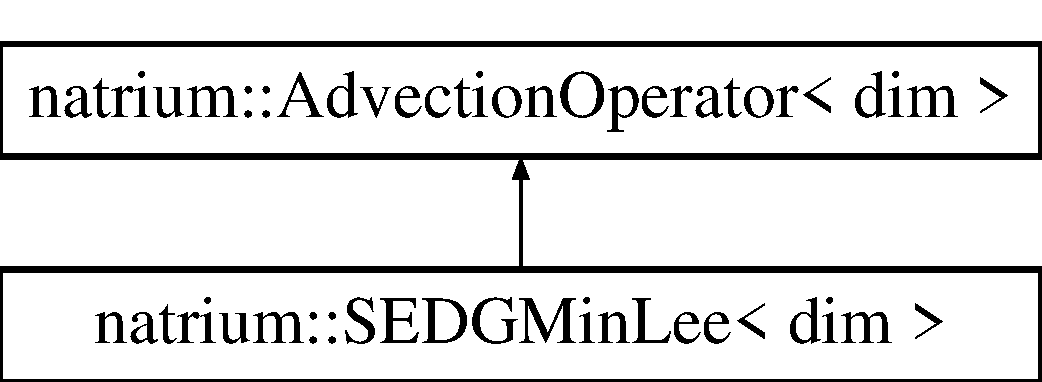
\includegraphics[height=2.000000cm]{classnatrium_1_1SEDGMinLee}
\end{center}
\end{figure}
\subsection*{Public Member Functions}
\begin{DoxyCompactItemize}
\item 
\hyperlink{classnatrium_1_1SEDGMinLee_a5bcf88b62420136630f78323b9b161b8}{S\-E\-D\-G\-Min\-Lee} (shared\-\_\-ptr$<$ dealii\-::\-Triangulation$<$ dim $>$ $>$ triangulation, shared\-\_\-ptr$<$ \hyperlink{classnatrium_1_1BoundaryCollection}{Boundary\-Collection}$<$ dim $>$ $>$ boundaries, size\-\_\-t order\-Of\-Finite\-Element, shared\-\_\-ptr$<$ \hyperlink{classnatrium_1_1BoltzmannModel}{Boltzmann\-Model} $>$ boltzmann\-Model, string input\-Directory=\char`\"{}\char`\"{}, bool use\-Central\-Flux=false)
\begin{DoxyCompactList}\small\item\em constructor \end{DoxyCompactList}\item 
\hypertarget{classnatrium_1_1SEDGMinLee_a6c55a31bc4cb0e314876af7251ad8ce3}{virtual \hyperlink{classnatrium_1_1SEDGMinLee_a6c55a31bc4cb0e314876af7251ad8ce3}{$\sim$\-S\-E\-D\-G\-Min\-Lee} ()}\label{classnatrium_1_1SEDGMinLee_a6c55a31bc4cb0e314876af7251ad8ce3}

\begin{DoxyCompactList}\small\item\em destructor \end{DoxyCompactList}\item 
virtual void \hyperlink{classnatrium_1_1SEDGMinLee_a5fa8b34df3c3bdd9f492a1e555effbe4}{reassemble} ()
\begin{DoxyCompactList}\small\item\em function to (re-\/)assemble linear system \end{DoxyCompactList}\item 
\hypertarget{classnatrium_1_1SEDGMinLee_a04707d696f7f466f17e3de055187ecd9}{virtual void \hyperlink{classnatrium_1_1SEDGMinLee_a04707d696f7f466f17e3de055187ecd9}{stream} ()}\label{classnatrium_1_1SEDGMinLee_a04707d696f7f466f17e3de055187ecd9}

\begin{DoxyCompactList}\small\item\em make streaming step \end{DoxyCompactList}\item 
virtual void \hyperlink{classnatrium_1_1SEDGMinLee_ab3cf80e18230ee7f08f4ed9883b9dadd}{save\-Checkpoint} (const string \&directory) const 
\begin{DoxyCompactList}\small\item\em save matrices and status to files \end{DoxyCompactList}\item 
\hypertarget{classnatrium_1_1SEDGMinLee_adcf3f6321cbf27f6c540a6c5f21c7cb0}{virtual const \\*
distributed\-\_\-sparse\-\_\-block\-\_\-matrix \& \hyperlink{classnatrium_1_1SEDGMinLee_adcf3f6321cbf27f6c540a6c5f21c7cb0}{get\-System\-Matrix} () const }\label{classnatrium_1_1SEDGMinLee_adcf3f6321cbf27f6c540a6c5f21c7cb0}

\begin{DoxyCompactList}\small\item\em get global system matrix \end{DoxyCompactList}\item 
\hypertarget{classnatrium_1_1SEDGMinLee_ab01fe7f989aed26cb5547eaba8ddb4ee}{virtual void {\bfseries map\-Do\-Fs\-To\-Support\-Points} (vector$<$ dealii\-::\-Point$<$ dim $>$ $>$ \&support\-Points) const }\label{classnatrium_1_1SEDGMinLee_ab01fe7f989aed26cb5547eaba8ddb4ee}

\item 
\hypertarget{classnatrium_1_1SEDGMinLee_a3ffd3d7bc5aae9dbb5a021d7e4913f65}{virtual const shared\-\_\-ptr\\*
$<$ dealii\-::\-Do\-F\-Handler$<$ dim $>$ $>$ \& {\bfseries get\-Do\-F\-Handler} () const }\label{classnatrium_1_1SEDGMinLee_a3ffd3d7bc5aae9dbb5a021d7e4913f65}

\item 
\hypertarget{classnatrium_1_1SEDGMinLee_a10acabaac20a992130e88fb9bd395d31}{const \\*
dealii\-::\-Block\-Sparsity\-Pattern \& {\bfseries get\-Block\-Sparsity\-Pattern} () const }\label{classnatrium_1_1SEDGMinLee_a10acabaac20a992130e88fb9bd395d31}

\item 
\hypertarget{classnatrium_1_1SEDGMinLee_ac9392932aaab8186b427b9d12bc64771}{const dealii\-::\-Sparsity\-Pattern \& {\bfseries get\-Sparsity\-Pattern} (size\-\_\-t i) const }\label{classnatrium_1_1SEDGMinLee_ac9392932aaab8186b427b9d12bc64771}

\item 
\hypertarget{classnatrium_1_1SEDGMinLee_a7d093da19c6796a3021f5d3f4beab542}{const dealii\-::\-Mapping\-Q1$<$ dim $>$ \& {\bfseries get\-Mapping} () const }\label{classnatrium_1_1SEDGMinLee_a7d093da19c6796a3021f5d3f4beab542}

\item 
\hypertarget{classnatrium_1_1SEDGMinLee_a8947d4078fadf1f71fcd7304210fa75c}{const std\-::map$<$ size\-\_\-t, size\-\_\-t $>$ \& {\bfseries get\-Celldof\-To\-Q\-Index} () const }\label{classnatrium_1_1SEDGMinLee_a8947d4078fadf1f71fcd7304210fa75c}

\item 
\hypertarget{classnatrium_1_1SEDGMinLee_a8b7d94c90ccfa5e341d854059d883f57}{const vector$<$ std\-::map$<$ size\-\_\-t, \\*
size\-\_\-t $>$ $>$ \& {\bfseries get\-Facedof\-To\-Q\-Index} () const }\label{classnatrium_1_1SEDGMinLee_a8b7d94c90ccfa5e341d854059d883f57}

\item 
\hypertarget{classnatrium_1_1SEDGMinLee_a653928dc9f0dd3715389b28196cab7bb}{const shared\-\_\-ptr\\*
$<$ dealii\-::\-Q\-Gauss\-Lobatto$<$ dim-\/1 $>$ $>$ \& {\bfseries get\-Face\-Quadrature} () const }\label{classnatrium_1_1SEDGMinLee_a653928dc9f0dd3715389b28196cab7bb}

\item 
\hypertarget{classnatrium_1_1SEDGMinLee_adb3df3ea790cb6a4d58dd9bed2e1ce1c}{const shared\-\_\-ptr\\*
$<$ dealii\-::\-F\-E\-\_\-\-D\-G\-Q\-Arbitrary\-Nodes\\*
$<$ dim $>$ $>$ \& {\bfseries get\-Fe} () const }\label{classnatrium_1_1SEDGMinLee_adb3df3ea790cb6a4d58dd9bed2e1ce1c}

\item 
\hypertarget{classnatrium_1_1SEDGMinLee_ad3ca0f23194a27d69d82d0f3ba89e345}{const shared\-\_\-ptr\\*
$<$ dealii\-::\-Q\-Gauss\-Lobatto$<$ dim $>$ $>$ \& {\bfseries get\-Quadrature} () const }\label{classnatrium_1_1SEDGMinLee_ad3ca0f23194a27d69d82d0f3ba89e345}

\item 
\hypertarget{classnatrium_1_1SEDGMinLee_a745a65de3ee72a250c0706e6c7fcc361}{size\-\_\-t {\bfseries get\-Order\-Of\-Finite\-Element} () const }\label{classnatrium_1_1SEDGMinLee_a745a65de3ee72a250c0706e6c7fcc361}

\item 
\hypertarget{classnatrium_1_1SEDGMinLee_af667cda1a894340f614da67c0a0ae5da}{virtual size\-\_\-t {\bfseries get\-Number\-Of\-Do\-Fs} () const }\label{classnatrium_1_1SEDGMinLee_af667cda1a894340f614da67c0a0ae5da}

\end{DoxyCompactItemize}


\subsection{Detailed Description}
\subsubsection*{template$<$size\-\_\-t dim$>$class natrium\-::\-S\-E\-D\-G\-Min\-Lee$<$ dim $>$}

This class solves the linear advection equations by a scheme which is used, e.\-g., by Min and Lee (2011)\-: A spectral-\/element discontinuous Galerkin lattice Boltzmann method for nearly incompressible flows, J\-C\-P 230 pp. 245-\/259. The advection equations used in the Lattice Boltzmann on unstructured grids are \[ \partial_t f_i + e_i \partial_x f_i = 0,\quad \forall i = 1,\dots,Q-1 \] where $ f_i(x,t) $ are the particle distribution functions, and $ e_i $ are the particle velocities. The discontinuous Galerkin (D\-G) method turns these P\-D\-Es into a large system of O\-D\-Es which can then be solved by a time integration scheme. Whereas this class implements the S\-E\-D\-G spatial discretization, the time integration is done by a subclass of \hyperlink{classnatrium_1_1TimeIntegrator}{Time\-Integrator}, e.\-g. \hyperlink{classnatrium_1_1RungeKutta5LowStorage}{Runge\-Kutta5\-Low\-Storage}. In other Finite Element schemes, degrees of freedom can belong to different elements (e.\-g. at corners of elements). In contrast, D\-G methods have the degrees of freedom belonging to a single element, which can lead to discontinuities at the element faces. To connect neighbor cells, the integral over the boundary of each cell incorporates the solution on neighbor cells. These contributions are called numerical fluxes. The D\-G scheme uses the weak formulation of the above equations on quadrilateral elements \$\$\-: \[ \left( \partial_t f_i + \partial_x (e_i f_i), \Phi \right)_{\Omega_e} = \left(n \left[ e_i f_i - F^{\ast}_{i}(f) \right], \Phi \right)_{\partial \Omega_e}. \] In this formulation $ F^{\ast}_{i}(f) $ denotes the numerical fluxes. They can be be calculated as central fluxes or Lax-\/\-Friedrichs fluxes. Lax-\/\-Friedrichs is in general more accurate for the advection equation. For detailed information on the fluxes, see the cited paper. For spatial integration a Gauss-\/\-Lobatto quadrature is used, which has the advantage that the resulting mass matrix M\-\_\-i = (, )\-\_\-\{\} is diagonal. This circumvents the solution of a linear equation system. including particle distributions f, system matrix L, diagonal mass matrix M, gradient matrices Dx, Dy, (Dz) and boundary matrix R. 


\begin{DoxyTemplParams}{Template Parameters}
{\em dim} & The dimension of the flow (2 or 3). \\
\hline
\end{DoxyTemplParams}


\subsection{Constructor \& Destructor Documentation}
\hypertarget{classnatrium_1_1SEDGMinLee_a5bcf88b62420136630f78323b9b161b8}{\index{natrium\-::\-S\-E\-D\-G\-Min\-Lee@{natrium\-::\-S\-E\-D\-G\-Min\-Lee}!S\-E\-D\-G\-Min\-Lee@{S\-E\-D\-G\-Min\-Lee}}
\index{S\-E\-D\-G\-Min\-Lee@{S\-E\-D\-G\-Min\-Lee}!natrium::SEDGMinLee@{natrium\-::\-S\-E\-D\-G\-Min\-Lee}}
\subsubsection[{S\-E\-D\-G\-Min\-Lee}]{\setlength{\rightskip}{0pt plus 5cm}template$<$size\-\_\-t dim$>$ template {\bf natrium\-::\-S\-E\-D\-G\-Min\-Lee}$<$ dim $>$\-::{\bf S\-E\-D\-G\-Min\-Lee} (
\begin{DoxyParamCaption}
\item[{shared\-\_\-ptr$<$ dealii\-::\-Triangulation$<$ dim $>$ $>$}]{triangulation, }
\item[{shared\-\_\-ptr$<$ {\bf Boundary\-Collection}$<$ dim $>$ $>$}]{boundaries, }
\item[{size\-\_\-t}]{order\-Of\-Finite\-Element, }
\item[{shared\-\_\-ptr$<$ {\bf Boltzmann\-Model} $>$}]{boltzmann\-Model, }
\item[{string}]{input\-Directory = {\ttfamily \char`\"{}\char`\"{}}, }
\item[{bool}]{use\-Central\-Flux = {\ttfamily false}}
\end{DoxyParamCaption}
)}}\label{classnatrium_1_1SEDGMinLee_a5bcf88b62420136630f78323b9b161b8}


constructor 

The template parameter must be made explicit in order for the code to compile.

Constructor 
\begin{DoxyParams}[1]{Parameters}
\mbox{\tt in}  & {\em triangulation} & The global mesh. \\
\hline
\mbox{\tt in}  & {\em order\-Of\-Finite\-Element} & The number of nodes element and dimension \\
\hline
\mbox{\tt in}  & {\em boltzmann\-Model} & the D\-Q model \\
\hline
\end{DoxyParams}


\subsection{Member Function Documentation}
\hypertarget{classnatrium_1_1SEDGMinLee_a5fa8b34df3c3bdd9f492a1e555effbe4}{\index{natrium\-::\-S\-E\-D\-G\-Min\-Lee@{natrium\-::\-S\-E\-D\-G\-Min\-Lee}!reassemble@{reassemble}}
\index{reassemble@{reassemble}!natrium::SEDGMinLee@{natrium\-::\-S\-E\-D\-G\-Min\-Lee}}
\subsubsection[{reassemble}]{\setlength{\rightskip}{0pt plus 5cm}template$<$size\-\_\-t dim$>$ template void {\bf natrium\-::\-S\-E\-D\-G\-Min\-Lee}$<$ dim $>$\-::reassemble (
\begin{DoxyParamCaption}
{}
\end{DoxyParamCaption}
)\hspace{0.3cm}{\ttfamily [virtual]}}}\label{classnatrium_1_1SEDGMinLee_a5fa8b34df3c3bdd9f492a1e555effbe4}


function to (re-\/)assemble linear system 

The template parameter must be made explicit in order for the code to compile. 

Implements \hyperlink{classnatrium_1_1AdvectionOperator_a89c25c3dae9a1e5973cd89fab8c2c052}{natrium\-::\-Advection\-Operator$<$ dim $>$}.

\hypertarget{classnatrium_1_1SEDGMinLee_ab3cf80e18230ee7f08f4ed9883b9dadd}{\index{natrium\-::\-S\-E\-D\-G\-Min\-Lee@{natrium\-::\-S\-E\-D\-G\-Min\-Lee}!save\-Checkpoint@{save\-Checkpoint}}
\index{save\-Checkpoint@{save\-Checkpoint}!natrium::SEDGMinLee@{natrium\-::\-S\-E\-D\-G\-Min\-Lee}}
\subsubsection[{save\-Checkpoint}]{\setlength{\rightskip}{0pt plus 5cm}template$<$size\-\_\-t dim$>$ template void {\bf natrium\-::\-S\-E\-D\-G\-Min\-Lee}$<$ dim $>$\-::save\-Checkpoint (
\begin{DoxyParamCaption}
\item[{const string \&}]{directory}
\end{DoxyParamCaption}
) const\hspace{0.3cm}{\ttfamily [virtual]}}}\label{classnatrium_1_1SEDGMinLee_ab3cf80e18230ee7f08f4ed9883b9dadd}


save matrices and status to files 


\begin{DoxyParams}[1]{Parameters}
\mbox{\tt in}  & {\em directory} & directory to save the matrix files to \\
\hline
\end{DoxyParams}

\begin{DoxyExceptions}{Exceptions}
{\em \hyperlink{classnatrium_1_1AdvectionSolverException}{Advection\-Solver\-Exception}} & \\
\hline
\end{DoxyExceptions}


Implements \hyperlink{classnatrium_1_1AdvectionOperator_aca14260bae100874b0050a2a96d7a564}{natrium\-::\-Advection\-Operator$<$ dim $>$}.



The documentation for this class was generated from the following files\-:\begin{DoxyCompactItemize}
\item 
/home/kraemer/eclipse\-\_\-workspace/\-N\-A\-Triu\-M/src/natrium/advection/\hyperlink{SEDGMinLee_8h}{S\-E\-D\-G\-Min\-Lee.\-h}\item 
/home/kraemer/eclipse\-\_\-workspace/\-N\-A\-Triu\-M/src/natrium/advection/\hyperlink{SEDGMinLee_8cpp}{S\-E\-D\-G\-Min\-Lee.\-cpp}\end{DoxyCompactItemize}

\hypertarget{classnatrium_1_1SolverConfiguration}{\section{natrium\-:\-:Solver\-Configuration Class Reference}
\label{classnatrium_1_1SolverConfiguration}\index{natrium\-::\-Solver\-Configuration@{natrium\-::\-Solver\-Configuration}}
}


Class that stores the configuration for a C\-F\-D simulation based on the Discrete Boltzmann Equation (D\-B\-E).  




{\ttfamily \#include $<$Solver\-Configuration.\-h$>$}

\subsection*{Public Member Functions}
\begin{DoxyCompactItemize}
\item 
\hypertarget{classnatrium_1_1SolverConfiguration_a9aa7109e2eac9b8a7b424a35509ccdb0}{\hyperlink{classnatrium_1_1SolverConfiguration_a9aa7109e2eac9b8a7b424a35509ccdb0}{Solver\-Configuration} ()}\label{classnatrium_1_1SolverConfiguration_a9aa7109e2eac9b8a7b424a35509ccdb0}

\begin{DoxyCompactList}\small\item\em constructor \end{DoxyCompactList}\item 
\hypertarget{classnatrium_1_1SolverConfiguration_ac1b521d8c205b8774dbb7c038304336d}{virtual \hyperlink{classnatrium_1_1SolverConfiguration_ac1b521d8c205b8774dbb7c038304336d}{$\sim$\-Solver\-Configuration} ()}\label{classnatrium_1_1SolverConfiguration_ac1b521d8c205b8774dbb7c038304336d}

\begin{DoxyCompactList}\small\item\em destructor \end{DoxyCompactList}\item 
void \hyperlink{classnatrium_1_1SolverConfiguration_a06547d0908d22a6f4f0bde286ba0c4fc}{check\-Configuration} ()
\begin{DoxyCompactList}\small\item\em Check if the configuration is consistent. \end{DoxyCompactList}\item 
void \hyperlink{classnatrium_1_1SolverConfiguration_a49e6c9cd57689289c79b47a6104b483a}{check\-Problem} (shared\-\_\-ptr$<$ \hyperlink{classnatrium_1_1ProblemDescription}{Problem\-Description}$<$ 2 $>$ $>$ c\-F\-D\-Problem)
\begin{DoxyCompactList}\small\item\em Check if the problem definition is in accordance with the solver configuration. \end{DoxyCompactList}\item 
void \hyperlink{classnatrium_1_1SolverConfiguration_af13da3022a9f995ce09b0918092da0c9}{check\-Problem} (shared\-\_\-ptr$<$ \hyperlink{classnatrium_1_1ProblemDescription}{Problem\-Description}$<$ 3 $>$ $>$ c\-F\-D\-Problem)
\begin{DoxyCompactList}\small\item\em Check if the problem definition is in accordance with the solver configuration. \end{DoxyCompactList}\item 
\hypertarget{classnatrium_1_1SolverConfiguration_a80b7bb1348a80859262bcd6c2bd9a92b}{Collision\-Type {\bfseries get\-Collision\-Type} () const }\label{classnatrium_1_1SolverConfiguration_a80b7bb1348a80859262bcd6c2bd9a92b}

\item 
\hypertarget{classnatrium_1_1SolverConfiguration_a81229d6067b27d7d5e3c2f54433a7356}{void {\bfseries set\-Collision\-Type} (Collision\-Type collision\-Type)}\label{classnatrium_1_1SolverConfiguration_a81229d6067b27d7d5e3c2f54433a7356}

\item 
\hypertarget{classnatrium_1_1SolverConfiguration_aa322f097289b1bf070f2eebac9a18dd2}{Stencil\-Type {\bfseries get\-Stencil\-Type} () const }\label{classnatrium_1_1SolverConfiguration_aa322f097289b1bf070f2eebac9a18dd2}

\item 
\hypertarget{classnatrium_1_1SolverConfiguration_a6551279c5aeff9df5a5b6580ae69434a}{void {\bfseries set\-Stencil\-Type} (Stencil\-Type stencil\-Type)}\label{classnatrium_1_1SolverConfiguration_a6551279c5aeff9df5a5b6580ae69434a}

\item 
\hypertarget{classnatrium_1_1SolverConfiguration_a7bee4e8ec36c072d0007df5596fdba62}{double {\bfseries get\-Time\-Step} () const }\label{classnatrium_1_1SolverConfiguration_a7bee4e8ec36c072d0007df5596fdba62}

\item 
\hypertarget{classnatrium_1_1SolverConfiguration_a07640346bb1525ed2e0c6272977920af}{void {\bfseries set\-Time\-Step} (double time\-Step)}\label{classnatrium_1_1SolverConfiguration_a07640346bb1525ed2e0c6272977920af}

\item 
\hypertarget{classnatrium_1_1SolverConfiguration_ac15089081763003182b3b60de135f0d4}{size\-\_\-t {\bfseries get\-Order\-Of\-Finite\-Element} () const }\label{classnatrium_1_1SolverConfiguration_ac15089081763003182b3b60de135f0d4}

\item 
\hypertarget{classnatrium_1_1SolverConfiguration_a4ac66a94dc9a300ce780ce17e3de8705}{void {\bfseries set\-Order\-Of\-Finite\-Element} (size\-\_\-t order\-Of\-Finite\-Element)}\label{classnatrium_1_1SolverConfiguration_a4ac66a94dc9a300ce780ce17e3de8705}

\item 
\hypertarget{classnatrium_1_1SolverConfiguration_a4f00a02f85ffd33640160e1adf894b2e}{Time\-Integrator\-Type {\bfseries get\-Time\-Integrator\-Type} () const }\label{classnatrium_1_1SolverConfiguration_a4f00a02f85ffd33640160e1adf894b2e}

\item 
\hypertarget{classnatrium_1_1SolverConfiguration_afaafedeee6d6bfad773b931c5373e969}{void {\bfseries set\-Time\-Integrator\-Type} (Time\-Integrator\-Type time\-Integrator\-Type)}\label{classnatrium_1_1SolverConfiguration_afaafedeee6d6bfad773b931c5373e969}

\item 
\hypertarget{classnatrium_1_1SolverConfiguration_a4fcdac4c96a9ad187b977cc5c1828e0e}{Advection\-Operator\-Type {\bfseries get\-Advection\-Operator\-Type} () const }\label{classnatrium_1_1SolverConfiguration_a4fcdac4c96a9ad187b977cc5c1828e0e}

\item 
\hypertarget{classnatrium_1_1SolverConfiguration_ae29272c0bf8fb87893ca9f4490b1e532}{void {\bfseries set\-Advection\-Operator\-Type} (Advection\-Operator\-Type advection\-Operator\-Type)}\label{classnatrium_1_1SolverConfiguration_ae29272c0bf8fb87893ca9f4490b1e532}

\item 
\hypertarget{classnatrium_1_1SolverConfiguration_a17f8418a66eb2df556ada3ac0897e3c4}{size\-\_\-t {\bfseries get\-Number\-Of\-Time\-Steps} () const }\label{classnatrium_1_1SolverConfiguration_a17f8418a66eb2df556ada3ac0897e3c4}

\item 
\hypertarget{classnatrium_1_1SolverConfiguration_a3e82a2c57d7a952f8f6e26838f07eefb}{void {\bfseries set\-Number\-Of\-Time\-Steps} (size\-\_\-t number\-Of\-Time\-Steps)}\label{classnatrium_1_1SolverConfiguration_a3e82a2c57d7a952f8f6e26838f07eefb}

\item 
\hypertarget{classnatrium_1_1SolverConfiguration_a8cb8f579ce1a4e9d5619795ae3598126}{Flux\-Type {\bfseries get\-Flux\-Type} () const }\label{classnatrium_1_1SolverConfiguration_a8cb8f579ce1a4e9d5619795ae3598126}

\item 
\hypertarget{classnatrium_1_1SolverConfiguration_aeef6044ffe9400d2214078b79a44343e}{void {\bfseries set\-Flux\-Type} (Flux\-Type flux\-Type)}\label{classnatrium_1_1SolverConfiguration_aeef6044ffe9400d2214078b79a44343e}

\item 
\hypertarget{classnatrium_1_1SolverConfiguration_a418057140bd0717a2e276a41328e043f}{const std\-::string \& {\bfseries get\-Output\-Directory} () const }\label{classnatrium_1_1SolverConfiguration_a418057140bd0717a2e276a41328e043f}

\item 
\hypertarget{classnatrium_1_1SolverConfiguration_acd249488bb83773514c4d6917b5bfc3a}{void {\bfseries set\-Output\-Directory} (const std\-::string \&output\-Directory)}\label{classnatrium_1_1SolverConfiguration_acd249488bb83773514c4d6917b5bfc3a}

\item 
\hypertarget{classnatrium_1_1SolverConfiguration_a2c71a2baa4134c00a9d51962c0858608}{double {\bfseries get\-D\-Q\-Scaling} () const }\label{classnatrium_1_1SolverConfiguration_a2c71a2baa4134c00a9d51962c0858608}

\item 
\hypertarget{classnatrium_1_1SolverConfiguration_a25f4b8ac9b325f455c5c273d75ed7551}{void {\bfseries set\-D\-Q\-Scaling} (double d\-Q\-Scaling)}\label{classnatrium_1_1SolverConfiguration_a25f4b8ac9b325f455c5c273d75ed7551}

\item 
\hypertarget{classnatrium_1_1SolverConfiguration_ac2edb568e16cf38fc7fa5aa0b45532ff}{int {\bfseries get\-Output\-Flags} () const }\label{classnatrium_1_1SolverConfiguration_ac2edb568e16cf38fc7fa5aa0b45532ff}

\item 
\hypertarget{classnatrium_1_1SolverConfiguration_a098031e207af99ebfadee20b4341eabd}{void {\bfseries set\-Output\-Flags} (int output\-Flags)}\label{classnatrium_1_1SolverConfiguration_a098031e207af99ebfadee20b4341eabd}

\item 
\hypertarget{classnatrium_1_1SolverConfiguration_a6bd8b754c338c4505b51c0ef3a1ebe37}{bool {\bfseries is\-Restart} () const }\label{classnatrium_1_1SolverConfiguration_a6bd8b754c338c4505b51c0ef3a1ebe37}

\item 
\hypertarget{classnatrium_1_1SolverConfiguration_afa537a3371bd51a7a042481df76a7c3b}{void {\bfseries set\-Restart} (bool restart)}\label{classnatrium_1_1SolverConfiguration_afa537a3371bd51a7a042481df76a7c3b}

\item 
\hypertarget{classnatrium_1_1SolverConfiguration_aada76bc5babb994525964b8a1143bb15}{Distribution\-Init\-Type {\bfseries get\-Distribution\-Init\-Type} () const }\label{classnatrium_1_1SolverConfiguration_aada76bc5babb994525964b8a1143bb15}

\item 
\hypertarget{classnatrium_1_1SolverConfiguration_aed9dc4e2b88e7a76998fed4e69b6c5dc}{void {\bfseries set\-Distribution\-Init\-Type} (Distribution\-Init\-Type distribution\-Init\-Type)}\label{classnatrium_1_1SolverConfiguration_aed9dc4e2b88e7a76998fed4e69b6c5dc}

\item 
\hypertarget{classnatrium_1_1SolverConfiguration_af1d809d9a559efda0a66736dcb64c430}{size\-\_\-t {\bfseries get\-Max\-Distribution\-Init\-Iterations} () const }\label{classnatrium_1_1SolverConfiguration_af1d809d9a559efda0a66736dcb64c430}

\item 
\hypertarget{classnatrium_1_1SolverConfiguration_a96aa9a31e4d4bee62df8d7bceccd6854}{void {\bfseries set\-Max\-Distribution\-Init\-Iterations} (size\-\_\-t max\-Distribution\-Init\-Iterations)}\label{classnatrium_1_1SolverConfiguration_a96aa9a31e4d4bee62df8d7bceccd6854}

\item 
\hypertarget{classnatrium_1_1SolverConfiguration_a26e733da8edd36afa784a19141dfa11e}{double {\bfseries get\-Stop\-Distribution\-Init\-Residual} () const }\label{classnatrium_1_1SolverConfiguration_a26e733da8edd36afa784a19141dfa11e}

\item 
\hypertarget{classnatrium_1_1SolverConfiguration_ad9689ce7a643360688906af1725f9105}{void {\bfseries set\-Stop\-Distribution\-Init\-Residual} (double stop\-Distribution\-Init\-Residual)}\label{classnatrium_1_1SolverConfiguration_ad9689ce7a643360688906af1725f9105}

\item 
\hypertarget{classnatrium_1_1SolverConfiguration_a00d3f2d230004ae0043c317222a8822e}{size\-\_\-t {\bfseries get\-Output\-Checkpoint\-Every} () const }\label{classnatrium_1_1SolverConfiguration_a00d3f2d230004ae0043c317222a8822e}

\item 
\hypertarget{classnatrium_1_1SolverConfiguration_a3d33552c3a6fb7cbdef3d63a739e5228}{void {\bfseries set\-Output\-Checkpoint\-Every} (size\-\_\-t output\-Checkpoint\-Every)}\label{classnatrium_1_1SolverConfiguration_a3d33552c3a6fb7cbdef3d63a739e5228}

\item 
\hypertarget{classnatrium_1_1SolverConfiguration_ab4da4ef57be63ec9c38d3f1d09d62402}{size\-\_\-t {\bfseries get\-Output\-Vector\-Fields\-Every} () const }\label{classnatrium_1_1SolverConfiguration_ab4da4ef57be63ec9c38d3f1d09d62402}

\item 
\hypertarget{classnatrium_1_1SolverConfiguration_a05d21fe7e83132ce9d216df3ff0e1e16}{void {\bfseries set\-Output\-Vector\-Fields\-Every} (size\-\_\-t output\-Vector\-Fields\-Every)}\label{classnatrium_1_1SolverConfiguration_a05d21fe7e83132ce9d216df3ff0e1e16}

\end{DoxyCompactItemize}


\subsection{Detailed Description}
Class that stores the configuration for a C\-F\-D simulation based on the Discrete Boltzmann Equation (D\-B\-E). 


\begin{DoxyTemplParams}{Template Parameters}
{\em dim} & The dimension of the flow (2 or 3). \\
\hline
\end{DoxyTemplParams}


\subsection{Member Function Documentation}
\hypertarget{classnatrium_1_1SolverConfiguration_a06547d0908d22a6f4f0bde286ba0c4fc}{\index{natrium\-::\-Solver\-Configuration@{natrium\-::\-Solver\-Configuration}!check\-Configuration@{check\-Configuration}}
\index{check\-Configuration@{check\-Configuration}!natrium::SolverConfiguration@{natrium\-::\-Solver\-Configuration}}
\subsubsection[{check\-Configuration}]{\setlength{\rightskip}{0pt plus 5cm}void natrium\-::\-Solver\-Configuration\-::check\-Configuration (
\begin{DoxyParamCaption}
{}
\end{DoxyParamCaption}
)\hspace{0.3cm}{\ttfamily [inline]}}}\label{classnatrium_1_1SolverConfiguration_a06547d0908d22a6f4f0bde286ba0c4fc}


Check if the configuration is consistent. 

Test writing permission on output directory If no restart\-: Check if checkpoint exists. If yes -\/$>$ ask for overwrite \hypertarget{classnatrium_1_1SolverConfiguration_a49e6c9cd57689289c79b47a6104b483a}{\index{natrium\-::\-Solver\-Configuration@{natrium\-::\-Solver\-Configuration}!check\-Problem@{check\-Problem}}
\index{check\-Problem@{check\-Problem}!natrium::SolverConfiguration@{natrium\-::\-Solver\-Configuration}}
\subsubsection[{check\-Problem}]{\setlength{\rightskip}{0pt plus 5cm}void natrium\-::\-Solver\-Configuration\-::check\-Problem (
\begin{DoxyParamCaption}
\item[{shared\-\_\-ptr$<$ {\bf Problem\-Description}$<$ 2 $>$ $>$}]{c\-F\-D\-Problem}
\end{DoxyParamCaption}
)\hspace{0.3cm}{\ttfamily [inline]}}}\label{classnatrium_1_1SolverConfiguration_a49e6c9cd57689289c79b47a6104b483a}


Check if the problem definition is in accordance with the solver configuration. 


\begin{DoxyParams}[1]{Parameters}
\mbox{\tt in}  & {\em c\-F\-D\-Problem} & Shared pointer to a problem description\\
\hline
\end{DoxyParams}

\begin{DoxyExceptions}{Exceptions}
{\em ...} & //\-T\-O\-D\-O implement custom exception \\
\hline
\end{DoxyExceptions}
\hypertarget{classnatrium_1_1SolverConfiguration_af13da3022a9f995ce09b0918092da0c9}{\index{natrium\-::\-Solver\-Configuration@{natrium\-::\-Solver\-Configuration}!check\-Problem@{check\-Problem}}
\index{check\-Problem@{check\-Problem}!natrium::SolverConfiguration@{natrium\-::\-Solver\-Configuration}}
\subsubsection[{check\-Problem}]{\setlength{\rightskip}{0pt plus 5cm}void natrium\-::\-Solver\-Configuration\-::check\-Problem (
\begin{DoxyParamCaption}
\item[{shared\-\_\-ptr$<$ {\bf Problem\-Description}$<$ 3 $>$ $>$}]{c\-F\-D\-Problem}
\end{DoxyParamCaption}
)\hspace{0.3cm}{\ttfamily [inline]}}}\label{classnatrium_1_1SolverConfiguration_af13da3022a9f995ce09b0918092da0c9}


Check if the problem definition is in accordance with the solver configuration. 


\begin{DoxyParams}[1]{Parameters}
\mbox{\tt in}  & {\em c\-F\-D\-Problem} & Shared pointer to a problem description\\
\hline
\end{DoxyParams}

\begin{DoxyExceptions}{Exceptions}
{\em ...} & //\-T\-O\-D\-O implement custom exception \\
\hline
\end{DoxyExceptions}


The documentation for this class was generated from the following file\-:\begin{DoxyCompactItemize}
\item 
/home/kraemer/eclipse\-\_\-workspace/\-N\-A\-Triu\-M/src/natrium/solver/\hyperlink{SolverConfiguration_8h}{Solver\-Configuration.\-h}\end{DoxyCompactItemize}

\hypertarget{classnatrium_1_1SteadyPeriodicTestFlow2D}{
\section{natrium::SteadyPeriodicTestFlow2D Class Reference}
\label{classnatrium_1_1SteadyPeriodicTestFlow2D}\index{natrium::SteadyPeriodicTestFlow2D@{natrium::SteadyPeriodicTestFlow2D}}
}


Description of a simple Periodic Flow (flow in square domain). The domain is \mbox{[}0,1\mbox{]}$^\wedge$2. The domain consists of 8 x 8 = 64 Elements (contrast to Min and Lee, who have 6 x 6).  


{\ttfamily \#include $<$PeriodicTestFlow2D.h$>$}Inheritance diagram for natrium::SteadyPeriodicTestFlow2D::\begin{figure}[H]
\begin{center}
\leavevmode
\includegraphics[height=3cm]{classnatrium_1_1SteadyPeriodicTestFlow2D}
\end{center}
\end{figure}
\subsection*{Classes}
\begin{DoxyCompactItemize}
\item 
class \hyperlink{classnatrium_1_1SteadyPeriodicTestFlow2D_1_1InitialVelocity}{InitialVelocity}
\end{DoxyCompactItemize}
\subsection*{Public Member Functions}
\begin{DoxyCompactItemize}
\item 
\hyperlink{classnatrium_1_1SteadyPeriodicTestFlow2D_a7db4598e86b34158612497ea2ff0ca74}{SteadyPeriodicTestFlow2D} (double viscosity, size\_\-t refinementLevel)
\begin{DoxyCompactList}\small\item\em constructor \item\end{DoxyCompactList}\item 
\hypertarget{classnatrium_1_1SteadyPeriodicTestFlow2D_a7344b71a404f2c4bbc73c1c738fdfa22}{
virtual \hyperlink{classnatrium_1_1SteadyPeriodicTestFlow2D_a7344b71a404f2c4bbc73c1c738fdfa22}{$\sim$SteadyPeriodicTestFlow2D} ()}
\label{classnatrium_1_1SteadyPeriodicTestFlow2D_a7344b71a404f2c4bbc73c1c738fdfa22}

\begin{DoxyCompactList}\small\item\em destructor \item\end{DoxyCompactList}\end{DoxyCompactItemize}


\subsection{Detailed Description}
Description of a simple Periodic Flow (flow in square domain). The domain is \mbox{[}0,1\mbox{]}$^\wedge$2. The domain consists of 8 x 8 = 64 Elements (contrast to Min and Lee, who have 6 x 6). 

\subsection{Constructor \& Destructor Documentation}
\hypertarget{classnatrium_1_1SteadyPeriodicTestFlow2D_a7db4598e86b34158612497ea2ff0ca74}{
\index{natrium::SteadyPeriodicTestFlow2D@{natrium::SteadyPeriodicTestFlow2D}!SteadyPeriodicTestFlow2D@{SteadyPeriodicTestFlow2D}}
\index{SteadyPeriodicTestFlow2D@{SteadyPeriodicTestFlow2D}!natrium::SteadyPeriodicTestFlow2D@{natrium::SteadyPeriodicTestFlow2D}}
\subsubsection[{SteadyPeriodicTestFlow2D}]{\setlength{\rightskip}{0pt plus 5cm}natrium::SteadyPeriodicTestFlow2D::SteadyPeriodicTestFlow2D (double {\em viscosity}, \/  size\_\-t {\em refinementLevel})\hspace{0.3cm}{\ttfamily  \mbox{[}inline\mbox{]}}}}
\label{classnatrium_1_1SteadyPeriodicTestFlow2D_a7db4598e86b34158612497ea2ff0ca74}


constructor 

apply boundary values 

The documentation for this class was generated from the following file:\begin{DoxyCompactItemize}
\item 
/mnt/fdrive/akraem3m/workspace/NATriuM/src/test/solver/\hyperlink{PeriodicTestFlow2D_8h}{PeriodicTestFlow2D.h}\end{DoxyCompactItemize}

\hypertarget{classnatrium_1_1TaylorGreenVortex2D}{
\section{natrium::TaylorGreenVortex2D Class Reference}
\label{classnatrium_1_1TaylorGreenVortex2D}\index{natrium::TaylorGreenVortex2D@{natrium::TaylorGreenVortex2D}}
}


Description of a simple Periodic Flow (flow in square domain). The domain is \mbox{[}0,1\mbox{]}$^\wedge$2. The domain consists of 8 x 8 = 64 Elements (contrast to Min and Lee, who have 6 x 6).  


{\ttfamily \#include $<$TaylorGreenVortex2D.h$>$}Inheritance diagram for natrium::TaylorGreenVortex2D::\begin{figure}[H]
\begin{center}
\leavevmode
\includegraphics[height=3cm]{classnatrium_1_1TaylorGreenVortex2D}
\end{center}
\end{figure}
\subsection*{Classes}
\begin{DoxyCompactItemize}
\item 
class \hyperlink{classnatrium_1_1TaylorGreenVortex2D_1_1AnalyticDensity}{AnalyticDensity}
\begin{DoxyCompactList}\small\item\em class to describe the y-\/component of the analytic solution \item\end{DoxyCompactList}\item 
class \hyperlink{classnatrium_1_1TaylorGreenVortex2D_1_1AnalyticVelocity}{AnalyticVelocity}
\begin{DoxyCompactList}\small\item\em class to describe the x-\/component of the analytic solution \item\end{DoxyCompactList}\end{DoxyCompactItemize}
\subsection*{Public Member Functions}
\begin{DoxyCompactItemize}
\item 
\hyperlink{classnatrium_1_1TaylorGreenVortex2D_a48410d029b8a0f9801b66efda45aa77f}{TaylorGreenVortex2D} (double viscosity, size\_\-t refinementLevel, double cs=0.57735026919, bool init\_\-rho\_\-analytically=false)
\begin{DoxyCompactList}\small\item\em constructor (with default cs=1/sqrt(3)) \item\end{DoxyCompactList}\item 
\hypertarget{classnatrium_1_1TaylorGreenVortex2D_abb6099f4f9791f7decabb35ccd3dbe49}{
virtual \hyperlink{classnatrium_1_1TaylorGreenVortex2D_abb6099f4f9791f7decabb35ccd3dbe49}{$\sim$TaylorGreenVortex2D} ()}
\label{classnatrium_1_1TaylorGreenVortex2D_abb6099f4f9791f7decabb35ccd3dbe49}

\begin{DoxyCompactList}\small\item\em destructor \item\end{DoxyCompactList}\end{DoxyCompactItemize}


\subsection{Detailed Description}
Description of a simple Periodic Flow (flow in square domain). The domain is \mbox{[}0,1\mbox{]}$^\wedge$2. The domain consists of 8 x 8 = 64 Elements (contrast to Min and Lee, who have 6 x 6). 

\subsection{Constructor \& Destructor Documentation}
\hypertarget{classnatrium_1_1TaylorGreenVortex2D_a48410d029b8a0f9801b66efda45aa77f}{
\index{natrium::TaylorGreenVortex2D@{natrium::TaylorGreenVortex2D}!TaylorGreenVortex2D@{TaylorGreenVortex2D}}
\index{TaylorGreenVortex2D@{TaylorGreenVortex2D}!natrium::TaylorGreenVortex2D@{natrium::TaylorGreenVortex2D}}
\subsubsection[{TaylorGreenVortex2D}]{\setlength{\rightskip}{0pt plus 5cm}natrium::TaylorGreenVortex2D::TaylorGreenVortex2D (double {\em viscosity}, \/  size\_\-t {\em refinementLevel}, \/  double {\em cs} = {\ttfamily 0.57735026919}, \/  bool {\em init\_\-rho\_\-analytically} = {\ttfamily false})}}
\label{classnatrium_1_1TaylorGreenVortex2D_a48410d029b8a0f9801b66efda45aa77f}


constructor (with default cs=1/sqrt(3)) 

apply boundary values 

The documentation for this class was generated from the following files:\begin{DoxyCompactItemize}
\item 
/mnt/fdrive/akraem3m/workspace/NATriuM/src/library/natrium/benchmarks/\hyperlink{TaylorGreenVortex2D_8h}{TaylorGreenVortex2D.h}\item 
/mnt/fdrive/akraem3m/workspace/NATriuM/src/library/natrium/benchmarks/\hyperlink{TaylorGreenVortex2D_8cpp}{TaylorGreenVortex2D.cpp}\end{DoxyCompactItemize}

\hypertarget{classnatrium_1_1TimeIntegrator}{
\section{natrium::TimeIntegrator$<$ MATRIX, VECTOR $>$ Class Template Reference}
\label{classnatrium_1_1TimeIntegrator}\index{natrium::TimeIntegrator@{natrium::TimeIntegrator}}
}


Abstract class for time integration (solution of ordinary differential equations (ODE)).  


{\ttfamily \#include $<$TimeIntegrator.h$>$}Inheritance diagram for natrium::TimeIntegrator$<$ MATRIX, VECTOR $>$::\begin{figure}[H]
\begin{center}
\leavevmode
\includegraphics[height=0.816327cm]{classnatrium_1_1TimeIntegrator}
\end{center}
\end{figure}
\subsection*{Public Member Functions}
\begin{DoxyCompactItemize}
\item 
\hypertarget{classnatrium_1_1TimeIntegrator_a420ea9baabf0839bc8ecb5f5e02ce95b}{
\hyperlink{classnatrium_1_1TimeIntegrator_a420ea9baabf0839bc8ecb5f5e02ce95b}{TimeIntegrator} (double timeStepSize)}
\label{classnatrium_1_1TimeIntegrator_a420ea9baabf0839bc8ecb5f5e02ce95b}

\begin{DoxyCompactList}\small\item\em constructor \item\end{DoxyCompactList}\item 
\hypertarget{classnatrium_1_1TimeIntegrator_a8795d06c5322b72a5a2a1f30aa7a051d}{
virtual \hyperlink{classnatrium_1_1TimeIntegrator_a8795d06c5322b72a5a2a1f30aa7a051d}{$\sim$TimeIntegrator} ()}
\label{classnatrium_1_1TimeIntegrator_a8795d06c5322b72a5a2a1f30aa7a051d}

\begin{DoxyCompactList}\small\item\em destructor \item\end{DoxyCompactList}\item 
\hypertarget{classnatrium_1_1TimeIntegrator_a6e763133e114cdd758307ca30b65f161}{
double {\bfseries getTimeStepSize} () const }
\label{classnatrium_1_1TimeIntegrator_a6e763133e114cdd758307ca30b65f161}

\item 
\hypertarget{classnatrium_1_1TimeIntegrator_a18592866e946c63ab1595d3ab688ea6b}{
void {\bfseries setTimeStepSize} (double timeStepSize)}
\label{classnatrium_1_1TimeIntegrator_a18592866e946c63ab1595d3ab688ea6b}

\item 
virtual double \hyperlink{classnatrium_1_1TimeIntegrator_a1c438e41d183d172d524aa5dc97785fb}{step} (VECTOR \&f, const MATRIX \&systemMatrix, const VECTOR \&systemVector, double t=0, double dt=0)=0
\begin{DoxyCompactList}\small\item\em make one time integration step on f: \[ \frac{df}{dt} = Af+b \]. \item\end{DoxyCompactList}\end{DoxyCompactItemize}


\subsection{Detailed Description}
\subsubsection*{template$<$class MATRIX, class VECTOR$>$ class natrium::TimeIntegrator$<$ MATRIX, VECTOR $>$}

Abstract class for time integration (solution of ordinary differential equations (ODE)). \begin{DoxyNote}{Note}
The ODEs arise from the space discretization of the DBE, which is basically a partial differential equation (PDE). By application of a space discretization scheme (like discontinuous Galerkin or standard FEM methods) the space derivatives in the PDE are replaced with arithmetic expressions. The only remaining derivative is then the time derivative, which makes the equation an ODE. The latter can be solved using classical time integration methods like Runge-\/Kutta or Adams-\/Moulton. 
\end{DoxyNote}


\subsection{Member Function Documentation}
\hypertarget{classnatrium_1_1TimeIntegrator_a1c438e41d183d172d524aa5dc97785fb}{
\index{natrium::TimeIntegrator@{natrium::TimeIntegrator}!step@{step}}
\index{step@{step}!natrium::TimeIntegrator@{natrium::TimeIntegrator}}
\subsubsection[{step}]{\setlength{\rightskip}{0pt plus 5cm}template$<$class MATRIX , class VECTOR $>$ virtual double {\bf natrium::TimeIntegrator}$<$ MATRIX, VECTOR $>$::step (VECTOR \& {\em f}, \/  const MATRIX \& {\em systemMatrix}, \/  const VECTOR \& {\em systemVector}, \/  double {\em t} = {\ttfamily 0}, \/  double {\em dt} = {\ttfamily 0})\hspace{0.3cm}{\ttfamily  \mbox{[}pure virtual\mbox{]}}}}
\label{classnatrium_1_1TimeIntegrator_a1c438e41d183d172d524aa5dc97785fb}


make one time integration step on f: \[ \frac{df}{dt} = Af+b \]. 
\begin{DoxyParams}{Parameters}
\item[{\em in/out\mbox{]}}]f Vector of degrees of freedom \item[\mbox{$\leftarrow$} {\em systemMatrix}]Matrix A \item[\mbox{$\leftarrow$} {\em systemVector}]Vector b \item[\mbox{$\leftarrow$} {\em double}]t global time \item[\mbox{$\leftarrow$} {\em double}]dt time step size. Required to interface deal.II's embedded RK methods \end{DoxyParams}
\begin{DoxyReturn}{Returns}
new global time 
\end{DoxyReturn}
\begin{DoxyNote}{Note}
fully virtual method. Overloaded by subclasses. 
\end{DoxyNote}


Implemented in \hyperlink{classnatrium_1_1DealIIWrapper_a62621205ff77a46c4f3ef01c3aefb06d}{natrium::DealIIWrapper$<$ MATRIX, VECTOR $>$}, \hyperlink{classnatrium_1_1ExponentialTimeIntegrator_ae0a9cff9bdafab123016db72d1439ef8}{natrium::ExponentialTimeIntegrator$<$ MATRIX, VECTOR $>$}, \hyperlink{classnatrium_1_1RungeKutta5LowStorage_a11ed7e7ef3b4a5e575452261bc783a21}{natrium::RungeKutta5LowStorage$<$ MATRIX, VECTOR $>$}, and \hyperlink{classnatrium_1_1ThetaMethod_a247c639f49a05904dae01b05115bc7e4}{natrium::ThetaMethod$<$ MATRIX, VECTOR $>$}.

The documentation for this class was generated from the following files:\begin{DoxyCompactItemize}
\item 
/mnt/fdrive/akraem3m/workspace/NATriuM/src/library/natrium/timeintegration/\hyperlink{TimeIntegrator_8h}{TimeIntegrator.h}\item 
/mnt/fdrive/akraem3m/workspace/NATriuM/src/library/natrium/timeintegration/\hyperlink{TimeIntegrator_8cpp}{TimeIntegrator.cpp}\end{DoxyCompactItemize}

\hypertarget{classnatrium_1_1UnsteadyPeriodicTestFlow2D}{
\section{natrium::UnsteadyPeriodicTestFlow2D Class Reference}
\label{classnatrium_1_1UnsteadyPeriodicTestFlow2D}\index{natrium::UnsteadyPeriodicTestFlow2D@{natrium::UnsteadyPeriodicTestFlow2D}}
}
Inheritance diagram for natrium::UnsteadyPeriodicTestFlow2D::\begin{figure}[H]
\begin{center}
\leavevmode
\includegraphics[height=3cm]{classnatrium_1_1UnsteadyPeriodicTestFlow2D}
\end{center}
\end{figure}
\subsection*{Classes}
\begin{DoxyCompactItemize}
\item 
class \hyperlink{classnatrium_1_1UnsteadyPeriodicTestFlow2D_1_1UnsteadyInitialVelocity}{UnsteadyInitialVelocity}
\end{DoxyCompactItemize}
\subsection*{Public Member Functions}
\begin{DoxyCompactItemize}
\item 
\hypertarget{classnatrium_1_1UnsteadyPeriodicTestFlow2D_a3a513d06c9018e78041cf8179ef2d80f}{
\hyperlink{classnatrium_1_1UnsteadyPeriodicTestFlow2D_a3a513d06c9018e78041cf8179ef2d80f}{UnsteadyPeriodicTestFlow2D} (double viscosity, size\_\-t refinementLevel)}
\label{classnatrium_1_1UnsteadyPeriodicTestFlow2D_a3a513d06c9018e78041cf8179ef2d80f}

\begin{DoxyCompactList}\small\item\em constructor \item\end{DoxyCompactList}\item 
\hypertarget{classnatrium_1_1UnsteadyPeriodicTestFlow2D_aa91ea175e2993bf00f8a48fded987c54}{
virtual \hyperlink{classnatrium_1_1UnsteadyPeriodicTestFlow2D_aa91ea175e2993bf00f8a48fded987c54}{$\sim$UnsteadyPeriodicTestFlow2D} ()}
\label{classnatrium_1_1UnsteadyPeriodicTestFlow2D_aa91ea175e2993bf00f8a48fded987c54}

\begin{DoxyCompactList}\small\item\em destructor \item\end{DoxyCompactList}\end{DoxyCompactItemize}


The documentation for this class was generated from the following file:\begin{DoxyCompactItemize}
\item 
/mnt/fdrive/akraem3m/workspace/NATriuM/src/test/solver/\hyperlink{PeriodicTestFlow2D_8h}{PeriodicTestFlow2D.h}\end{DoxyCompactItemize}

\chapter{File Documentation}
\hypertarget{advectionConvergence_8cpp}{
\section{/mnt/fdrive/akraem3m/workspace/NATriuM/src/analysis/convergence-\/analysis-\/advection-\/solver/advectionConvergence.cpp File Reference}
\label{advectionConvergence_8cpp}\index{/mnt/fdrive/akraem3m/workspace/NATriuM/src/analysis/convergence-\/analysis-\/advection-\/solver/advectionConvergence.cpp@{/mnt/fdrive/akraem3m/workspace/NATriuM/src/analysis/convergence-\/analysis-\/advection-\/solver/advectionConvergence.cpp}}
}


Checks the convergence of the SEDG advection solver, analyzes the local discretization error in dependence of dt, dx and fe\_\-order.  
{\ttfamily \#include $<$fstream$>$}\par
{\ttfamily \#include $<$dirent.h$>$}\par
{\ttfamily \#include $<$sys/stat.h$>$}\par
{\ttfamily \#include $<$stdlib.h$>$}\par
{\ttfamily \#include \char`\"{}natrium/benchmarks/AdvectionBenchmark.h\char`\"{}}\par
\subsection*{Functions}
\begin{DoxyCompactItemize}
\item 
\hypertarget{advectionConvergence_8cpp_ae66f6b31b5ad750f1fe042a706a4e3d4}{
int {\bfseries main} ()}
\label{advectionConvergence_8cpp_ae66f6b31b5ad750f1fe042a706a4e3d4}

\end{DoxyCompactItemize}
\subsection*{Variables}
\begin{DoxyCompactItemize}
\item 
\hypertarget{advectionConvergence_8cpp_a51723df66b6d2d73c6a170e78775ae94}{
const bool {\bfseries OUTPUT} = false}
\label{advectionConvergence_8cpp_a51723df66b6d2d73c6a170e78775ae94}

\item 
\hypertarget{advectionConvergence_8cpp_a4cc6e74830c62cdcf030d4548e929d7a}{
const bool {\bfseries SMOOTH} = true}
\label{advectionConvergence_8cpp_a4cc6e74830c62cdcf030d4548e929d7a}

\end{DoxyCompactItemize}


\subsection{Detailed Description}
Checks the convergence of the SEDG advection solver, analyzes the local discretization error in dependence of dt, dx and fe\_\-order. \begin{DoxyDate}{Date}
13.02.2014 
\end{DoxyDate}
\begin{DoxyAuthor}{Author}
Andreas Kraemer, Bonn-\/Rhein-\/Sieg University of Applied Sciences, Sankt Augustin 
\end{DoxyAuthor}

\hypertarget{step-1_8cpp}{\section{/home/kraemer/eclipse\-\_\-workspace/\-N\-A\-Triu\-M/src/examples/step-\/1/step-\/1.cpp File Reference}
\label{step-1_8cpp}\index{/home/kraemer/eclipse\-\_\-workspace/\-N\-A\-Triu\-M/src/examples/step-\/1/step-\/1.\-cpp@{/home/kraemer/eclipse\-\_\-workspace/\-N\-A\-Triu\-M/src/examples/step-\/1/step-\/1.\-cpp}}
}


Taylor-\/\-Green vortex in 2\-D (only periodic walls)  


{\ttfamily \#include $<$fstream$>$}\\*
{\ttfamily \#include $<$time.\-h$>$}\\*
{\ttfamily \#include $<$stdlib.\-h$>$}\\*
{\ttfamily \#include \char`\"{}deal.\-I\-I/numerics/data\-\_\-out.\-h\char`\"{}}\\*
{\ttfamily \#include \char`\"{}solver/\-Benchmark\-C\-F\-D\-Solver.\-h\char`\"{}}\\*
{\ttfamily \#include \char`\"{}solver/\-Solver\-Configuration.\-h\char`\"{}}\\*
{\ttfamily \#include \char`\"{}problemdescription/\-Benchmark.\-h\char`\"{}}\\*
{\ttfamily \#include \char`\"{}utilities/\-Basic\-Names.\-h\char`\"{}}\\*
{\ttfamily \#include \char`\"{}Taylor\-Green\-Vortex2\-D.\-h\char`\"{}}\\*
\subsection*{Functions}
\begin{DoxyCompactItemize}
\item 
\hypertarget{step-1_8cpp_ae66f6b31b5ad750f1fe042a706a4e3d4}{int {\bfseries main} ()}\label{step-1_8cpp_ae66f6b31b5ad750f1fe042a706a4e3d4}

\end{DoxyCompactItemize}


\subsection{Detailed Description}
Taylor-\/\-Green vortex in 2\-D (only periodic walls) \begin{DoxyDate}{Date}
05.\-06.\-2014 
\end{DoxyDate}
\begin{DoxyAuthor}{Author}
Andreas Kraemer, Bonn-\/\-Rhein-\/\-Sieg University of Applied Sciences, Sankt Augustin 
\end{DoxyAuthor}

\hypertarget{TaylorGreenVortex2D_8cpp}{
\section{/mnt/fdrive/akraem3m/workspace/NATriuM/src/library/natrium/benchmarks/TaylorGreenVortex2D.cpp File Reference}
\label{TaylorGreenVortex2D_8cpp}\index{/mnt/fdrive/akraem3m/workspace/NATriuM/src/library/natrium/benchmarks/TaylorGreenVortex2D.cpp@{/mnt/fdrive/akraem3m/workspace/NATriuM/src/library/natrium/benchmarks/TaylorGreenVortex2D.cpp}}
}
{\ttfamily \#include \char`\"{}TaylorGreenVortex2D.h\char`\"{}}\par
{\ttfamily \#include \char`\"{}deal.II/grid/grid\_\-generator.h\char`\"{}}\par
{\ttfamily \#include \char`\"{}deal.II/grid/tria\_\-accessor.h\char`\"{}}\par
{\ttfamily \#include \char`\"{}deal.II/grid/tria\_\-iterator.h\char`\"{}}\par
{\ttfamily \#include \char`\"{}../boundaries/PeriodicBoundary.h\char`\"{}}\par
{\ttfamily \#include \char`\"{}../utilities/Math.h\char`\"{}}\par
\subsection*{Namespaces}
\begin{DoxyCompactItemize}
\item 
namespace \hyperlink{namespacenatrium}{natrium}


\begin{DoxyCompactList}\small\item\em Definition of Grad's function to reconstruct missing distribution functions, e.g. at boundaries. \item\end{DoxyCompactList}\end{DoxyCompactItemize}


\subsection{Detailed Description}
\begin{DoxyDate}{Date}
29.05.2013 
\end{DoxyDate}
\begin{DoxyAuthor}{Author}
Andreas Kraemer, Bonn-\/Rhein-\/Sieg University of Applied Sciences, Sankt Augustin 
\end{DoxyAuthor}

\hypertarget{TaylorGreenVortex2D_8h}{\section{/home/kraemer/eclipse\-\_\-workspace/\-N\-A\-Triu\-M/src/examples/step-\/1/\-Taylor\-Green\-Vortex2\-D.h File Reference}
\label{TaylorGreenVortex2D_8h}\index{/home/kraemer/eclipse\-\_\-workspace/\-N\-A\-Triu\-M/src/examples/step-\/1/\-Taylor\-Green\-Vortex2\-D.\-h@{/home/kraemer/eclipse\-\_\-workspace/\-N\-A\-Triu\-M/src/examples/step-\/1/\-Taylor\-Green\-Vortex2\-D.\-h}}
}


Description of a simple Periodic Flow (in rectangular domain).  


{\ttfamily \#include \char`\"{}deal.\-I\-I/grid/tria.\-h\char`\"{}}\\*
{\ttfamily \#include \char`\"{}problemdescription/\-Problem\-Description.\-h\char`\"{}}\\*
{\ttfamily \#include \char`\"{}utilities/\-Basic\-Names.\-h\char`\"{}}\\*
\subsection*{Classes}
\begin{DoxyCompactItemize}
\item 
class \hyperlink{classnatrium_1_1TaylorGreenVortex2D}{natrium\-::\-Taylor\-Green\-Vortex2\-D}
\begin{DoxyCompactList}\small\item\em Description of a simple Periodic Flow (flow in square domain). The domain is \mbox{[}0,1\mbox{]}$^\wedge$2. The domain consists of 8 x 8 = 64 Elements (contrast to Min and Lee, who have 6 x 6). \end{DoxyCompactList}\end{DoxyCompactItemize}


\subsection{Detailed Description}
Description of a simple Periodic Flow (in rectangular domain). \begin{DoxyDate}{Date}
29.\-05.\-2013 
\end{DoxyDate}
\begin{DoxyAuthor}{Author}
Andreas Kraemer, Bonn-\/\-Rhein-\/\-Sieg University of Applied Sciences, Sankt Augustin 
\end{DoxyAuthor}

\hypertarget{PoiseuilleFlow2D_8cpp}{\section{/home/kraemer/eclipse\-\_\-workspace/\-N\-A\-Triu\-M/src/examples/step-\/5/\-Poiseuille\-Flow2\-D.cpp File Reference}
\label{PoiseuilleFlow2D_8cpp}\index{/home/kraemer/eclipse\-\_\-workspace/\-N\-A\-Triu\-M/src/examples/step-\/5/\-Poiseuille\-Flow2\-D.\-cpp@{/home/kraemer/eclipse\-\_\-workspace/\-N\-A\-Triu\-M/src/examples/step-\/5/\-Poiseuille\-Flow2\-D.\-cpp}}
}
{\ttfamily \#include \char`\"{}Poiseuille\-Flow2\-D.\-h\char`\"{}}\\*
{\ttfamily \#include \char`\"{}deal.\-I\-I/grid/grid\-\_\-generator.\-h\char`\"{}}\\*
{\ttfamily \#include \char`\"{}deal.\-I\-I/grid/tria\-\_\-accessor.\-h\char`\"{}}\\*
{\ttfamily \#include \char`\"{}deal.\-I\-I/grid/tria\-\_\-iterator.\-h\char`\"{}}\\*
{\ttfamily \#include \char`\"{}problemdescription/\-Periodic\-Boundary.\-h\char`\"{}}\\*
{\ttfamily \#include \char`\"{}utilities/\-Math.\-h\char`\"{}}\\*


\subsection{Detailed Description}
\begin{DoxyDate}{Date}
29.\-05.\-2013 
\end{DoxyDate}
\begin{DoxyAuthor}{Author}
Andreas Kraemer, Bonn-\/\-Rhein-\/\-Sieg University of Applied Sciences, Sankt Augustin 
\end{DoxyAuthor}

\hypertarget{PoiseuilleFlow2D_8h}{
\section{/mnt/fdrive/akraem3m/workspace/NATriuM/src/library/natrium/benchmarks/PoiseuilleFlow2D.h File Reference}
\label{PoiseuilleFlow2D_8h}\index{/mnt/fdrive/akraem3m/workspace/NATriuM/src/library/natrium/benchmarks/PoiseuilleFlow2D.h@{/mnt/fdrive/akraem3m/workspace/NATriuM/src/library/natrium/benchmarks/PoiseuilleFlow2D.h}}
}


Channel flow in 2D.  
{\ttfamily \#include \char`\"{}deal.II/grid/tria.h\char`\"{}}\par
{\ttfamily \#include \char`\"{}deal.II/base/function.h\char`\"{}}\par
{\ttfamily \#include \char`\"{}../problemdescription/Benchmark.h\char`\"{}}\par
{\ttfamily \#include \char`\"{}../utilities/BasicNames.h\char`\"{}}\par
\subsection*{Classes}
\begin{DoxyCompactItemize}
\item 
class \hyperlink{classnatrium_1_1PoiseuilleFlow2D}{natrium::PoiseuilleFlow2D}
\begin{DoxyCompactList}\small\item\em Description of a simple Channel Flow The domain is \mbox{[}0,5\mbox{]}x\mbox{[}0,1\mbox{]}. \item\end{DoxyCompactList}\item 
class \hyperlink{classnatrium_1_1PoiseuilleFlow2D_1_1AnalyticVelocity}{natrium::PoiseuilleFlow2D::AnalyticVelocity}
\begin{DoxyCompactList}\small\item\em class to describe the x-\/component of the analytic solution \item\end{DoxyCompactList}\end{DoxyCompactItemize}
\subsection*{Namespaces}
\begin{DoxyCompactItemize}
\item 
namespace \hyperlink{namespacenatrium}{natrium}


\begin{DoxyCompactList}\small\item\em Definition of Grad's function to reconstruct missing distribution functions, e.g. at boundaries. \item\end{DoxyCompactList}\end{DoxyCompactItemize}


\subsection{Detailed Description}
Channel flow in 2D. \begin{DoxyDate}{Date}
29.05.2013 
\end{DoxyDate}
\begin{DoxyAuthor}{Author}
Andreas Kraemer, Bonn-\/Rhein-\/Sieg University of Applied Sciences, Sankt Augustin 
\end{DoxyAuthor}

\hypertarget{CouetteFlow2D_8cpp}{
\section{/mnt/fdrive/akraem3m/workspace/NATriuM/src/library/natrium/benchmarks/CouetteFlow2D.cpp File Reference}
\label{CouetteFlow2D_8cpp}\index{/mnt/fdrive/akraem3m/workspace/NATriuM/src/library/natrium/benchmarks/CouetteFlow2D.cpp@{/mnt/fdrive/akraem3m/workspace/NATriuM/src/library/natrium/benchmarks/CouetteFlow2D.cpp}}
}
{\ttfamily \#include \char`\"{}CouetteFlow2D.h\char`\"{}}\par
{\ttfamily \#include \char`\"{}deal.II/grid/grid\_\-generator.h\char`\"{}}\par
{\ttfamily \#include \char`\"{}deal.II/grid/grid\_\-tools.h\char`\"{}}\par
{\ttfamily \#include \char`\"{}deal.II/grid/grid\_\-out.h\char`\"{}}\par
{\ttfamily \#include \char`\"{}deal.II/grid/tria\_\-accessor.h\char`\"{}}\par
{\ttfamily \#include \char`\"{}deal.II/grid/tria\_\-iterator.h\char`\"{}}\par
{\ttfamily \#include \char`\"{}deal.II/base/geometry\_\-info.h\char`\"{}}\par
{\ttfamily \#include \char`\"{}../problemdescription/PeriodicBoundary.h\char`\"{}}\par
{\ttfamily \#include \char`\"{}../problemdescription/LinearBoundaryRhoU.h\char`\"{}}\par
{\ttfamily \#include \char`\"{}../utilities/Logging.h\char`\"{}}\par
{\ttfamily \#include \char`\"{}../utilities/MPIGuard.h\char`\"{}}\par


\subsection{Detailed Description}
\begin{DoxyDate}{Date}
29.05.2013 
\end{DoxyDate}
\begin{DoxyAuthor}{Author}
Andreas Kraemer, Bonn-\/Rhein-\/Sieg University of Applied Sciences, Sankt Augustin 
\end{DoxyAuthor}

\hypertarget{CouetteFlow2D_8h}{\section{/home/kraemer/eclipse\-\_\-workspace/\-N\-A\-Triu\-M/src/examples/step-\/3/\-Couette\-Flow2\-D.h File Reference}
\label{CouetteFlow2D_8h}\index{/home/kraemer/eclipse\-\_\-workspace/\-N\-A\-Triu\-M/src/examples/step-\/3/\-Couette\-Flow2\-D.\-h@{/home/kraemer/eclipse\-\_\-workspace/\-N\-A\-Triu\-M/src/examples/step-\/3/\-Couette\-Flow2\-D.\-h}}
}


Description of a simple Couette Flow (regular channel flow in rectangular domain).  


{\ttfamily \#include \char`\"{}deal.\-I\-I/grid/tria.\-h\char`\"{}}\\*
{\ttfamily \#include \char`\"{}problemdescription/\-Problem\-Description.\-h\char`\"{}}\\*
{\ttfamily \#include \char`\"{}utilities/\-Basic\-Names.\-h\char`\"{}}\\*
\subsection*{Classes}
\begin{DoxyCompactItemize}
\item 
class \hyperlink{classnatrium_1_1CouetteFlow2D}{natrium\-::\-Couette\-Flow2\-D}
\begin{DoxyCompactList}\small\item\em Description of a simple Couette Flow (regular channel flow in square domain). The domain is \mbox{[}0,1\mbox{]}$^\wedge$2. The top plate is moved with constant velocity. The domain consists of 8 x 8 = 64 Elements (contrast to Min and Lee, who have 6 x 6). \end{DoxyCompactList}\end{DoxyCompactItemize}


\subsection{Detailed Description}
Description of a simple Couette Flow (regular channel flow in rectangular domain). \begin{DoxyDate}{Date}
29.\-05.\-2013 
\end{DoxyDate}
\begin{DoxyAuthor}{Author}
Andreas Kraemer, Bonn-\/\-Rhein-\/\-Sieg University of Applied Sciences, Sankt Augustin 
\end{DoxyAuthor}

\hypertarget{step-3_8cpp}{\section{/home/kraemer/eclipse\-\_\-workspace/\-N\-A\-Triu\-M/src/examples/step-\/5/step-\/3.cpp File Reference}
\label{step-3_8cpp}\index{/home/kraemer/eclipse\-\_\-workspace/\-N\-A\-Triu\-M/src/examples/step-\/5/step-\/3.\-cpp@{/home/kraemer/eclipse\-\_\-workspace/\-N\-A\-Triu\-M/src/examples/step-\/5/step-\/3.\-cpp}}
}


Tutorial\-: Lid-\/\-Driven Cavity in 2\-D This example is thoroughly commented to introduce you to the key concepts in fluid flow simulations with N\-A\-Triu\-M. There are three main classes that are used in a N\-A\-Triu\-M simulation\-:  


{\ttfamily \#include $<$fstream$>$}\\*
{\ttfamily \#include \char`\"{}deal.\-I\-I/numerics/data\-\_\-out.\-h\char`\"{}}\\*
{\ttfamily \#include \char`\"{}solver/\-C\-F\-D\-Solver.\-h\char`\"{}}\\*
{\ttfamily \#include \char`\"{}solver/\-Solver\-Configuration.\-h\char`\"{}}\\*
{\ttfamily \#include \char`\"{}problemdescription/\-Problem\-Description.\-h\char`\"{}}\\*
{\ttfamily \#include \char`\"{}utilities/\-Basic\-Names.\-h\char`\"{}}\\*
{\ttfamily \#include \char`\"{}Poiseuille\-Flow2\-D.\-h\char`\"{}}\\*
\subsection*{Functions}
\begin{DoxyCompactItemize}
\item 
\hypertarget{step-3_8cpp_a34a3c1505f1afc2a3d8186abd7b11475}{void {\bfseries get\-Analytic\-Solution} (double time, distributed\-\_\-vector \&analytic\-Solution1, distributed\-\_\-vector \&analytic\-Solution2, const vector$<$ dealii\-::\-Point$<$ 2 $>$ $>$ \&support\-Points, const \hyperlink{classnatrium_1_1PoiseuilleFlow2D}{Poiseuille\-Flow2\-D} \&poi\-Flow)}\label{step-3_8cpp_a34a3c1505f1afc2a3d8186abd7b11475}

\item 
\hypertarget{step-3_8cpp_ae66f6b31b5ad750f1fe042a706a4e3d4}{int {\bfseries main} ()}\label{step-3_8cpp_ae66f6b31b5ad750f1fe042a706a4e3d4}

\end{DoxyCompactItemize}


\subsection{Detailed Description}
Tutorial\-: Lid-\/\-Driven Cavity in 2\-D This example is thoroughly commented to introduce you to the key concepts in fluid flow simulations with N\-A\-Triu\-M. There are three main classes that are used in a N\-A\-Triu\-M simulation\-: 
\begin{DoxyItemize}
\item Solver\-Configuration\-: Contains all the simulation preferences.
\item Problem\-Description\-: Contains the computation grid, initial conditions and boundary conditions. Problem\-Description is an abstract class with the purely virtual functions appy\-Initial\-Densities and apply\-Initial\-Velocities. When you use N\-A\-Triu\-M as a library, this class has to be overriden by a problem specific child class (here the class Lid\-Driven\-Cavity2\-D), which implements the virtual functions.
\item C\-F\-D\-Solver\-: The C\-F\-D\-Solver is the central class in the N\-A\-Triu\-M framework. It creates all necessary classes and runs the simulation. \begin{DoxyDate}{Date}
31.\-03.\-2014 
\end{DoxyDate}
\begin{DoxyAuthor}{Author}
Andreas Kraemer, Bonn-\/\-Rhein-\/\-Sieg University of Applied Sciences, Sankt Augustin 
\end{DoxyAuthor}

\end{DoxyItemize}
\hypertarget{AdvectionOperator_8cpp}{
\section{/mnt/fdrive/akraem3m/workspace/NATriuM/src/library/natrium/advection/AdvectionOperator.cpp File Reference}
\label{AdvectionOperator_8cpp}\index{/mnt/fdrive/akraem3m/workspace/NATriuM/src/library/natrium/advection/AdvectionOperator.cpp@{/mnt/fdrive/akraem3m/workspace/NATriuM/src/library/natrium/advection/AdvectionOperator.cpp}}
}
{\ttfamily \#include \char`\"{}AdvectionOperator.h\char`\"{}}\par


\subsection{Detailed Description}
\begin{DoxyDate}{Date}
29.05.2013 
\end{DoxyDate}
\begin{DoxyAuthor}{Author}
Andreas Kraemer, Bonn-\/Rhein-\/Sieg University of Applied Sciences, Sankt Augustin 
\end{DoxyAuthor}

\hypertarget{AdvectionOperator_8h}{\section{/home/kraemer/eclipse\-\_\-workspace/\-N\-A\-Triu\-M/src/natrium/advection/\-Advection\-Operator.h File Reference}
\label{AdvectionOperator_8h}\index{/home/kraemer/eclipse\-\_\-workspace/\-N\-A\-Triu\-M/src/natrium/advection/\-Advection\-Operator.\-h@{/home/kraemer/eclipse\-\_\-workspace/\-N\-A\-Triu\-M/src/natrium/advection/\-Advection\-Operator.\-h}}
}


Abstract class for spatial part of the Advection Operator e\-\_\-i $\ast$ dx\-\_\-i f.  


{\ttfamily \#include \char`\"{}../utilities/\-Basic\-Names.\-h\char`\"{}}\\*
\subsection*{Classes}
\begin{DoxyCompactItemize}
\item 
class \hyperlink{classnatrium_1_1AdvectionOperator}{natrium\-::\-Advection\-Operator$<$ dim $>$}
\begin{DoxyCompactList}\small\item\em Abstract class for spatial part of the Advection Operator e\-\_\-i $\ast$ dx\-\_\-i f. \end{DoxyCompactList}\end{DoxyCompactItemize}


\subsection{Detailed Description}
Abstract class for spatial part of the Advection Operator e\-\_\-i $\ast$ dx\-\_\-i f. \begin{DoxyDate}{Date}
29.\-05.\-2013 
\end{DoxyDate}
\begin{DoxyAuthor}{Author}
Andreas Kraemer, Bonn-\/\-Rhein-\/\-Sieg University of Applied Sciences, Sankt Augustin 
\end{DoxyAuthor}

\hypertarget{SEDGMinLee_8cpp}{
\section{/mnt/fdrive/akraem3m/workspace/NATriuM/src/library/natrium/advection/SEDGMinLee.cpp File Reference}
\label{SEDGMinLee_8cpp}\index{/mnt/fdrive/akraem3m/workspace/NATriuM/src/library/natrium/advection/SEDGMinLee.cpp@{/mnt/fdrive/akraem3m/workspace/NATriuM/src/library/natrium/advection/SEDGMinLee.cpp}}
}


Advection scheme proposed by Min and Lee (2011).  
{\ttfamily \#include \char`\"{}SEDGMinLee.h\char`\"{}}\par
{\ttfamily \#include $<$fstream$>$}\par
{\ttfamily \#include \char`\"{}deal.II/lac/dynamic\_\-sparsity\_\-pattern.h\char`\"{}}\par
{\ttfamily \#include \char`\"{}deal.II/dofs/dof\_\-renumbering.h\char`\"{}}\par
{\ttfamily \#include \char`\"{}deal.II/grid/tria\_\-accessor.h\char`\"{}}\par
{\ttfamily \#include \char`\"{}deal.II/grid/tria\_\-iterator.h\char`\"{}}\par
{\ttfamily \#include \char`\"{}deal.II/fe/fe\_\-update\_\-flags.h\char`\"{}}\par
{\ttfamily \#include \char`\"{}deal.II/lac/matrix\_\-iterator.h\char`\"{}}\par
{\ttfamily \#include \char`\"{}deal.II/lac/sparsity\_\-tools.h\char`\"{}}\par
{\ttfamily \#include \char`\"{}deal.II/base/utilities.h\char`\"{}}\par
{\ttfamily \#include \char`\"{}deal.II/lac/constraint\_\-matrix.h\char`\"{}}\par
{\ttfamily \#include \char`\"{}../problemdescription/PeriodicBoundary.h\char`\"{}}\par
{\ttfamily \#include \char`\"{}../problemdescription/LinearBoundary.h\char`\"{}}\par
{\ttfamily \#include \char`\"{}../stencils/Stencil.h\char`\"{}}\par
{\ttfamily \#include \char`\"{}../utilities/DealiiExtensions.h\char`\"{}}\par


\subsection{Detailed Description}
Advection scheme proposed by Min and Lee (2011). \begin{DoxyDate}{Date}
29.05.2013 
\end{DoxyDate}
\begin{DoxyAuthor}{Author}
Andreas Kraemer, Bonn-\/Rhein-\/Sieg University of Applied Sciences, Sankt Augustin 
\end{DoxyAuthor}

\hypertarget{SEDGMinLee_8h}{\section{/home/kraemer/eclipse\-\_\-workspace/\-N\-A\-Triu\-M/src/natrium/advection/\-S\-E\-D\-G\-Min\-Lee.h File Reference}
\label{SEDGMinLee_8h}\index{/home/kraemer/eclipse\-\_\-workspace/\-N\-A\-Triu\-M/src/natrium/advection/\-S\-E\-D\-G\-Min\-Lee.\-h@{/home/kraemer/eclipse\-\_\-workspace/\-N\-A\-Triu\-M/src/natrium/advection/\-S\-E\-D\-G\-Min\-Lee.\-h}}
}


Advection operator proposed by Min and Lee (2011)\-: A spectral-\/elemennt discontinuous Galerkin lattice Boltzmann method for nearly incompressible flows, J\-C\-P 230 pp. 245-\/259.  


{\ttfamily \#include $<$map$>$}\\*
{\ttfamily \#include \char`\"{}deal.\-I\-I/grid/tria.\-h\char`\"{}}\\*
{\ttfamily \#include \char`\"{}deal.\-I\-I/fe/fe\-\_\-dgq.\-h\char`\"{}}\\*
{\ttfamily \#include \char`\"{}deal.\-I\-I/dofs/dof\-\_\-handler.\-h\char`\"{}}\\*
{\ttfamily \#include $<$deal.\-I\-I/dofs/dof\-\_\-tools.\-h$>$}\\*
{\ttfamily \#include \char`\"{}deal.\-I\-I/lac/sparse\-\_\-matrix.\-h\char`\"{}}\\*
{\ttfamily \#include \char`\"{}deal.\-I\-I/lac/block\-\_\-sparsity\-\_\-pattern.\-h\char`\"{}}\\*
{\ttfamily \#include \char`\"{}deal.\-I\-I/base/quadrature\-\_\-lib.\-h\char`\"{}}\\*
{\ttfamily \#include \char`\"{}Advection\-Operator.\-h\char`\"{}}\\*
{\ttfamily \#include \char`\"{}../problemdescription/\-Boundary\-Collection.\-h\char`\"{}}\\*
{\ttfamily \#include \char`\"{}../boltzmannmodels/\-Boltzmann\-Model.\-h\char`\"{}}\\*
{\ttfamily \#include \char`\"{}../utilities/\-Basic\-Names.\-h\char`\"{}}\\*
\subsection*{Classes}
\begin{DoxyCompactItemize}
\item 
class \hyperlink{classnatrium_1_1AdvectionSolverException}{natrium\-::\-Advection\-Solver\-Exception}
\begin{DoxyCompactList}\small\item\em Exception class for Advection\-Solver. \end{DoxyCompactList}\item 
class \hyperlink{classnatrium_1_1SEDGMinLee}{natrium\-::\-S\-E\-D\-G\-Min\-Lee$<$ dim $>$}
\begin{DoxyCompactList}\small\item\em This class solves the linear advection equations by a scheme which is used, e.\-g., by Min and Lee (2011)\-: A spectral-\/element discontinuous Galerkin lattice Boltzmann method for nearly incompressible flows, J\-C\-P 230 pp. 245-\/259. The advection equations used in the Lattice Boltzmann on unstructured grids are \[ \partial_t f_i + e_i \partial_x f_i = 0,\quad \forall i = 1,\dots,Q-1 \] where $ f_i(x,t) $ are the particle distribution functions, and $ e_i $ are the particle velocities. The discontinuous Galerkin (D\-G) method turns these P\-D\-Es into a large system of O\-D\-Es which can then be solved by a time integration scheme. Whereas this class implements the S\-E\-D\-G spatial discretization, the time integration is done by a subclass of \hyperlink{classnatrium_1_1TimeIntegrator}{Time\-Integrator}, e.\-g. \hyperlink{classnatrium_1_1RungeKutta5LowStorage}{Runge\-Kutta5\-Low\-Storage}. In other Finite Element schemes, degrees of freedom can belong to different elements (e.\-g. at corners of elements). In contrast, D\-G methods have the degrees of freedom belonging to a single element, which can lead to discontinuities at the element faces. To connect neighbor cells, the integral over the boundary of each cell incorporates the solution on neighbor cells. These contributions are called numerical fluxes. The D\-G scheme uses the weak formulation of the above equations on quadrilateral elements \$\$\-: \[ \left( \partial_t f_i + \partial_x (e_i f_i), \Phi \right)_{\Omega_e} = \left(n \left[ e_i f_i - F^{\ast}_{i}(f) \right], \Phi \right)_{\partial \Omega_e}. \] In this formulation $ F^{\ast}_{i}(f) $ denotes the numerical fluxes. They can be be calculated as central fluxes or Lax-\/\-Friedrichs fluxes. Lax-\/\-Friedrichs is in general more accurate for the advection equation. For detailed information on the fluxes, see the cited paper. For spatial integration a Gauss-\/\-Lobatto quadrature is used, which has the advantage that the resulting mass matrix M\-\_\-i = (, )\-\_\-\{\} is diagonal. This circumvents the solution of a linear equation system. Each advection equation leads to a O\-D\-E \[ \partial_t f_i = M_i^{-1}(- e_{ix} D_{ix} - e_{iy} D_{iy} + R_i) f_i + B_i f_{i^{\ast}} + b_i.\] Altogether, for the example of the D2\-Q9, the system becomes \[ \partial_t f_{1,\dots,Q} = \left( \matrix{ L_1 & 0 & B_1 & 0 & 0 & 0 & 0 & 0 \cr 0 & L_2 & 0 & B_2 & 0 & 0 & 0 & 0 \cr B_3 & 0 & L_3 & 0 & 0 & 0 & 0 & 0 \cr 0 & B_4 & 0 & L_4 & 0 & 0 & 0 & 0 \cr 0 & 0 & 0 & 0 & L_5 & 0 & B_5 & 0 \cr 0 & 0 & 0 & 0 & 0 & L_6 & 0 & B_6\cr 0 & 0 & 0 & 0 & B_7 & 0 & L_7 & 0 \cr 0 & 0 & 0 & 0 & 0 & B_8 & 0 & L_8 } \right) f_{1,\dots,Q} + \left( \matrix{ b_1 \cr b_2 \cr b_3 \cr b_4 \cr b_5 \cr b_6 \cr b_7 \cr b_8 }\right), \] where $ L_i = M_i^{-1}(- e_{ix} D_{ix} - e_{iy} D_{iy} + R_i) $. \end{DoxyCompactList}\end{DoxyCompactItemize}


\subsection{Detailed Description}
Advection operator proposed by Min and Lee (2011)\-: A spectral-\/elemennt discontinuous Galerkin lattice Boltzmann method for nearly incompressible flows, J\-C\-P 230 pp. 245-\/259. \begin{DoxyDate}{Date}
29.\-05.\-2013 
\end{DoxyDate}
\begin{DoxyAuthor}{Author}
Andreas Kraemer, Bonn-\/\-Rhein-\/\-Sieg University of Applied Sciences, Sankt Augustin 
\end{DoxyAuthor}

\hypertarget{BoltzmannModel_8cpp}{\section{/home/kraemer/eclipse\-\_\-workspace/\-N\-A\-Triu\-M/src/natrium/boltzmannmodels/\-Boltzmann\-Model.cpp File Reference}
\label{BoltzmannModel_8cpp}\index{/home/kraemer/eclipse\-\_\-workspace/\-N\-A\-Triu\-M/src/natrium/boltzmannmodels/\-Boltzmann\-Model.\-cpp@{/home/kraemer/eclipse\-\_\-workspace/\-N\-A\-Triu\-M/src/natrium/boltzmannmodels/\-Boltzmann\-Model.\-cpp}}
}


Abstract class for the description of a boltzmann model.  


{\ttfamily \#include \char`\"{}Boltzmann\-Model.\-h\char`\"{}}\\*


\subsection{Detailed Description}
Abstract class for the description of a boltzmann model. \begin{DoxyDate}{Date}
04.\-06.\-2013 
\end{DoxyDate}
\begin{DoxyAuthor}{Author}
Andreas Kraemer, Bonn-\/\-Rhein-\/\-Sieg University of Applied Sciences, Sankt Augustin 
\end{DoxyAuthor}

\hypertarget{BoltzmannModel_8h}{\section{/home/kraemer/eclipse\-\_\-workspace/\-N\-A\-Triu\-M/src/natrium/boltzmannmodels/\-Boltzmann\-Model.h File Reference}
\label{BoltzmannModel_8h}\index{/home/kraemer/eclipse\-\_\-workspace/\-N\-A\-Triu\-M/src/natrium/boltzmannmodels/\-Boltzmann\-Model.\-h@{/home/kraemer/eclipse\-\_\-workspace/\-N\-A\-Triu\-M/src/natrium/boltzmannmodels/\-Boltzmann\-Model.\-h}}
}


Abstract class for the description of a boltzmann model.  


{\ttfamily \#include \char`\"{}assert.\-h\char`\"{}}\\*
{\ttfamily \#include \char`\"{}../utilities/\-Math.\-h\char`\"{}}\\*
{\ttfamily \#include \char`\"{}../utilities/\-Basic\-Names.\-h\char`\"{}}\\*
\subsection*{Classes}
\begin{DoxyCompactItemize}
\item 
class \hyperlink{classnatrium_1_1BoltzmannModel}{natrium\-::\-Boltzmann\-Model}
\begin{DoxyCompactList}\small\item\em Abstract class for the description of a boltzmann model, e.\-g. D2\-Q9. \end{DoxyCompactList}\end{DoxyCompactItemize}
\subsection*{Enumerations}
\begin{DoxyCompactItemize}
\item 
enum {\bfseries Stencil\-Type} \{ {\bfseries natrium\-::\-Stencil\-\_\-\-D2\-Q9}
 \}
\begin{DoxyCompactList}\small\item\em Enum type for the difference stencil. \end{DoxyCompactList}\end{DoxyCompactItemize}


\subsection{Detailed Description}
Abstract class for the description of a boltzmann model. \begin{DoxyDate}{Date}
04.\-06.\-2013 
\end{DoxyDate}
\begin{DoxyAuthor}{Author}
Andreas Kraemer, Bonn-\/\-Rhein-\/\-Sieg University of Applied Sciences, Sankt Augustin 
\end{DoxyAuthor}

\hypertarget{D2Q9Model_8cpp}{\section{/home/kraemer/eclipse\-\_\-workspace/\-N\-A\-Triu\-M/src/natrium/boltzmannmodels/\-D2\-Q9\-Model.cpp File Reference}
\label{D2Q9Model_8cpp}\index{/home/kraemer/eclipse\-\_\-workspace/\-N\-A\-Triu\-M/src/natrium/boltzmannmodels/\-D2\-Q9\-Model.\-cpp@{/home/kraemer/eclipse\-\_\-workspace/\-N\-A\-Triu\-M/src/natrium/boltzmannmodels/\-D2\-Q9\-Model.\-cpp}}
}
{\ttfamily \#include \char`\"{}D2\-Q9\-Model.\-h\char`\"{}}\\*
{\ttfamily \#include $<$math.\-h$>$}\\*
{\ttfamily \#include \char`\"{}boost/assign/std/vector.\-hpp\char`\"{}}\\*


\subsection{Detailed Description}
\begin{DoxyDate}{Date}
30.\-08.\-2013 
\end{DoxyDate}
\begin{DoxyAuthor}{Author}
Andreas Kraemer, Bonn-\/\-Rhein-\/\-Sieg University of Applied Sciences, Sankt Augustin 
\end{DoxyAuthor}

\hypertarget{D2Q9Model_8h}{\section{/home/kraemer/eclipse\-\_\-workspace/\-N\-A\-Triu\-M/src/natrium/boltzmannmodels/\-D2\-Q9\-Model.h File Reference}
\label{D2Q9Model_8h}\index{/home/kraemer/eclipse\-\_\-workspace/\-N\-A\-Triu\-M/src/natrium/boltzmannmodels/\-D2\-Q9\-Model.\-h@{/home/kraemer/eclipse\-\_\-workspace/\-N\-A\-Triu\-M/src/natrium/boltzmannmodels/\-D2\-Q9\-Model.\-h}}
}


D2\-Q9 Boltzmann Model.  


{\ttfamily \#include \char`\"{}Boltzmann\-Model.\-h\char`\"{}}\\*
{\ttfamily \#include \char`\"{}../utilities/\-Basic\-Names.\-h\char`\"{}}\\*
\subsection*{Classes}
\begin{DoxyCompactItemize}
\item 
class \hyperlink{classnatrium_1_1D2Q9Model}{natrium\-::\-D2\-Q9\-Model}
\begin{DoxyCompactList}\small\item\em D2\-Q9 Model. \end{DoxyCompactList}\end{DoxyCompactItemize}


\subsection{Detailed Description}
D2\-Q9 Boltzmann Model. \begin{DoxyDate}{Date}
02.\-06.\-2013 
\end{DoxyDate}
\begin{DoxyAuthor}{Author}
Andreas Kraemer, Bonn-\/\-Rhein-\/\-Sieg University of Applied Sciences, Sankt Augustin 
\end{DoxyAuthor}

\hypertarget{BGKTransformed_8cpp}{\section{/home/kraemer/eclipse\-\_\-workspace/\-N\-A\-Triu\-M/src/collisionmodels/\-B\-G\-K\-Transformed.cpp \-File \-Reference}
\label{BGKTransformed_8cpp}\index{/home/kraemer/eclipse\-\_\-workspace/\-N\-A\-Triu\-M/src/collisionmodels/\-B\-G\-K\-Transformed.\-cpp@{/home/kraemer/eclipse\-\_\-workspace/\-N\-A\-Triu\-M/src/collisionmodels/\-B\-G\-K\-Transformed.\-cpp}}
}
{\ttfamily \#include \char`\"{}\-B\-G\-K\-Transformed.\-h\char`\"{}}\*


\subsection{\-Detailed \-Description}
\begin{DoxyDate}{\-Date}
29.\-05.\-2013 
\end{DoxyDate}
\begin{DoxyAuthor}{\-Author}
\-Andreas \-Kraemer, \-Bonn-\/\-Rhein-\/\-Sieg \-University of \-Applied \-Sciences, \-Sankt \-Augustin 
\end{DoxyAuthor}

\hypertarget{BGKTransformed_8h}{\section{/home/kraemer/eclipse\-\_\-workspace/\-N\-A\-Triu\-M/src/natrium/collisionmodels/\-B\-G\-K\-Transformed.h File Reference}
\label{BGKTransformed_8h}\index{/home/kraemer/eclipse\-\_\-workspace/\-N\-A\-Triu\-M/src/natrium/collisionmodels/\-B\-G\-K\-Transformed.\-h@{/home/kraemer/eclipse\-\_\-workspace/\-N\-A\-Triu\-M/src/natrium/collisionmodels/\-B\-G\-K\-Transformed.\-h}}
}


Description of the B\-G\-K model for the transformed particle distributions, as described in Global data which is used by Min and Lee (2011)\-: A spectral-\/elemennt discontinuous Galerkin lattice Boltzmann method for nearly incompressible flows, J\-C\-P 230 pp. 245-\/259.  


{\ttfamily \#include \char`\"{}Collision\-Model.\-h\char`\"{}}\\*
{\ttfamily \#include \char`\"{}../utilities/\-Basic\-Names.\-h\char`\"{}}\\*
\subsection*{Classes}
\begin{DoxyCompactItemize}
\item 
class \hyperlink{classnatrium_1_1BGKTransformed}{natrium\-::\-B\-G\-K\-Transformed}
\begin{DoxyCompactList}\small\item\em Description of the B\-G\-K model for the transformed particle distributions, as described in Global data which is used by Min and Lee (2011)\-: A spectral-\/element discontinuous Galerkin lattice Boltzmann method for nearly incompressible flows, J\-C\-P 230 pp. 245-\/259. \end{DoxyCompactList}\end{DoxyCompactItemize}


\subsection{Detailed Description}
Description of the B\-G\-K model for the transformed particle distributions, as described in Global data which is used by Min and Lee (2011)\-: A spectral-\/elemennt discontinuous Galerkin lattice Boltzmann method for nearly incompressible flows, J\-C\-P 230 pp. 245-\/259. \begin{DoxyDate}{Date}
29.\-05.\-2013 
\end{DoxyDate}
\begin{DoxyAuthor}{Author}
Andreas Kraemer, Bonn-\/\-Rhein-\/\-Sieg University of Applied Sciences, Sankt Augustin 
\end{DoxyAuthor}

\hypertarget{CollisionModel_8cpp}{
\section{/mnt/fdrive/akraem3m/workspace/NATriuM/src/library/natrium/collision/CollisionModel.cpp File Reference}
\label{CollisionModel_8cpp}\index{/mnt/fdrive/akraem3m/workspace/NATriuM/src/library/natrium/collision/CollisionModel.cpp@{/mnt/fdrive/akraem3m/workspace/NATriuM/src/library/natrium/collision/CollisionModel.cpp}}
}
{\ttfamily \#include \char`\"{}CollisionModel.h\char`\"{}}\par


\subsection{Detailed Description}
\begin{DoxyDate}{Date}
29.05.2013 
\end{DoxyDate}
\begin{DoxyAuthor}{Author}
Andreas Kraemer, Bonn-\/Rhein-\/Sieg University of Applied Sciences, Sankt Augustin 
\end{DoxyAuthor}

\hypertarget{CollisionModel_8h}{\section{/home/kraemer/eclipse\-\_\-workspace/\-N\-A\-Triu\-M/src/collisionmodels/\-Collision\-Model.h \-File \-Reference}
\label{CollisionModel_8h}\index{/home/kraemer/eclipse\-\_\-workspace/\-N\-A\-Triu\-M/src/collisionmodels/\-Collision\-Model.\-h@{/home/kraemer/eclipse\-\_\-workspace/\-N\-A\-Triu\-M/src/collisionmodels/\-Collision\-Model.\-h}}
}


\-Abstract class for the description of collision schemes.  


{\ttfamily \#include \char`\"{}boost/shared\-\_\-ptr.\-hpp\char`\"{}}\*
{\ttfamily \#include \char`\"{}../boltzmannmodels/\-Boltzmann\-Model.\-h\char`\"{}}\*
{\ttfamily \#include \char`\"{}../utilities/\-Basic\-Names.\-h\char`\"{}}\*
\subsection*{\-Classes}
\begin{DoxyCompactItemize}
\item 
class \hyperlink{classnatrium_1_1CollisionModel}{natrium\-::\-Collision\-Model}
\begin{DoxyCompactList}\small\item\em \-Abstract class for the description of collision schemes. \end{DoxyCompactList}\end{DoxyCompactItemize}


\subsection{\-Detailed \-Description}
\-Abstract class for the description of collision schemes. \begin{DoxyDate}{\-Date}
29.\-05.\-2013 
\end{DoxyDate}
\begin{DoxyAuthor}{\-Author}
\-Andreas \-Kraemer, \-Bonn-\/\-Rhein-\/\-Sieg \-University of \-Applied \-Sciences, \-Sankt \-Augustin 
\end{DoxyAuthor}

\hypertarget{Boundary_8cpp}{\section{/home/kraemer/eclipse\-\_\-workspace/\-N\-A\-Triu\-M/src/natrium/problemdescription/\-Boundary.cpp File Reference}
\label{Boundary_8cpp}\index{/home/kraemer/eclipse\-\_\-workspace/\-N\-A\-Triu\-M/src/natrium/problemdescription/\-Boundary.\-cpp@{/home/kraemer/eclipse\-\_\-workspace/\-N\-A\-Triu\-M/src/natrium/problemdescription/\-Boundary.\-cpp}}
}


Abstract class for the description of boundary conditions.  


{\ttfamily \#include \char`\"{}Boundary.\-h\char`\"{}}\\*


\subsection{Detailed Description}
Abstract class for the description of boundary conditions. \begin{DoxyDate}{Date}
24.\-10.\-2013 
\end{DoxyDate}
\begin{DoxyAuthor}{Author}
Andreas Kraemer, Bonn-\/\-Rhein-\/\-Sieg University of Applied Sciences, Sankt Augustin 
\end{DoxyAuthor}

\hypertarget{Boundary_8h}{\section{/home/kraemer/eclipse\-\_\-workspace/\-N\-A\-Triu\-M/src/natrium/problemdescription/\-Boundary.h File Reference}
\label{Boundary_8h}\index{/home/kraemer/eclipse\-\_\-workspace/\-N\-A\-Triu\-M/src/natrium/problemdescription/\-Boundary.\-h@{/home/kraemer/eclipse\-\_\-workspace/\-N\-A\-Triu\-M/src/natrium/problemdescription/\-Boundary.\-h}}
}


Abstract class for Description of a Boundary object.  


{\ttfamily \#include \char`\"{}deal.\-I\-I/grid/tria.\-h\char`\"{}}\\*
{\ttfamily \#include \char`\"{}deal.\-I\-I/dofs/dof\-\_\-handler.\-h\char`\"{}}\\*
{\ttfamily \#include \char`\"{}deal.\-I\-I/fe/fe\-\_\-values.\-h\char`\"{}}\\*
{\ttfamily \#include \char`\"{}../utilities/\-Basic\-Names.\-h\char`\"{}}\\*
\subsection*{Classes}
\begin{DoxyCompactItemize}
\item 
class \hyperlink{classnatrium_1_1Boundary}{natrium\-::\-Boundary$<$ dim $>$}
\begin{DoxyCompactList}\small\item\em Abstract class for the description of boundaries. Base class of \hyperlink{classnatrium_1_1PeriodicBoundary}{Periodic\-Boundary}, Inflow\-Boundary, etc. \end{DoxyCompactList}\end{DoxyCompactItemize}


\subsection{Detailed Description}
Abstract class for Description of a Boundary object. \begin{DoxyDate}{Date}
24.\-10.\-2013 
\end{DoxyDate}
\begin{DoxyAuthor}{Author}
Andreas Kraemer, Bonn-\/\-Rhein-\/\-Sieg University of Applied Sciences, Sankt Augustin 
\end{DoxyAuthor}

\hypertarget{BoundaryTools_8cpp}{\section{/home/kraemer/eclipse\-\_\-workspace/\-N\-A\-Triu\-M/src/natrium/problemdescription/\-Boundary\-Tools.cpp File Reference}
\label{BoundaryTools_8cpp}\index{/home/kraemer/eclipse\-\_\-workspace/\-N\-A\-Triu\-M/src/natrium/problemdescription/\-Boundary\-Tools.\-cpp@{/home/kraemer/eclipse\-\_\-workspace/\-N\-A\-Triu\-M/src/natrium/problemdescription/\-Boundary\-Tools.\-cpp}}
}
{\ttfamily \#include \char`\"{}Boundary\-Tools.\-h\char`\"{}}\\*
{\ttfamily \#include \char`\"{}../utilities/\-Math.\-h\char`\"{}}\\*


\subsection{Detailed Description}
\begin{DoxyDate}{Date}
14.\-11.\-2013 
\end{DoxyDate}
\begin{DoxyAuthor}{Author}
Andreas Kraemer, Bonn-\/\-Rhein-\/\-Sieg University of Applied Sciences, Sankt Augustin 
\end{DoxyAuthor}

\hypertarget{BoundaryTools_8h}{
\section{/mnt/fdrive/akraem3m/workspace/NATriuM/src/library/natrium/problemdescription/BoundaryTools.h File Reference}
\label{BoundaryTools_8h}\index{/mnt/fdrive/akraem3m/workspace/NATriuM/src/library/natrium/problemdescription/BoundaryTools.h@{/mnt/fdrive/akraem3m/workspace/NATriuM/src/library/natrium/problemdescription/BoundaryTools.h}}
}
{\ttfamily \#include $<$string$>$}\par
{\ttfamily \#include \char`\"{}deal.II/base/point.h\char`\"{}}\par
{\ttfamily \#include \char`\"{}../utilities/BasicNames.h\char`\"{}}\par
\subsection*{Classes}
\begin{DoxyCompactItemize}
\item 
class \hyperlink{classnatrium_1_1BoundaryTools_1_1point__sorter}{natrium::BoundaryTools::point\_\-sorter}
\begin{DoxyCompactList}\small\item\em function to compare points as map keys; the points with smaller x components fall before others. in case of equal x, the points with smaller y components will be placed first. \item\end{DoxyCompactList}\end{DoxyCompactItemize}
\subsection*{Functions}
\begin{DoxyCompactItemize}
\item 
bool \hyperlink{namespacenatrium_1_1BoundaryTools_a64669bd0ddcea4f0eb21121beebcf76f}{natrium::BoundaryTools::checkParallelLines} (const dealii::Point$<$ 2 $>$ \&beginLine1, const dealii::Point$<$ 2 $>$ \&endLine1, dealii::Point$<$ 2 $>$ \&beginLine2, dealii::Point$<$ 2 $>$ \&endLine2, std::string \&errorMessage)
\begin{DoxyCompactList}\small\item\em Check if two lines in a 2D plane are parallel and not equal to each other. If they are antiparallel, swap begin and end of the second line. \item\end{DoxyCompactList}\item 
bool \hyperlink{namespacenatrium_1_1BoundaryTools_a4e8c575691fa9a235b59807cc3d2686a}{natrium::BoundaryTools::getInterfacialLinesByBoundaryIndicator} (size\_\-t boundaryIndicator1, size\_\-t boundaryIndicator2, shared\_\-ptr$<$ Mesh$<$ 2 $>$ $>$ triangulation, dealii::Point$<$ 2 $>$ \&beginLine1, dealii::Point$<$ 2 $>$ \&endLine1, dealii::Point$<$ 2 $>$ \&beginLine2, dealii::Point$<$ 2 $>$ \&endLine2, std::string \&errorMessage)
\begin{DoxyCompactList}\small\item\em Get the positions of the lines that define interfaces from the defining \hyperlink{classnatrium_1_1Boundary}{Boundary} indicators. \item\end{DoxyCompactList}\end{DoxyCompactItemize}


\subsection{Detailed Description}
\begin{DoxyDate}{Date}
14.11.2013 
\end{DoxyDate}
\begin{DoxyAuthor}{Author}
Andreas Kraemer, Bonn-\/Rhein-\/Sieg University of Applied Sciences, Sankt Augustin 
\end{DoxyAuthor}

\hypertarget{PeriodicBoundary_8cpp}{\section{/home/kraemer/eclipse\-\_\-workspace/\-N\-A\-Triu\-M/src/natrium/problemdescription/\-Periodic\-Boundary.cpp File Reference}
\label{PeriodicBoundary_8cpp}\index{/home/kraemer/eclipse\-\_\-workspace/\-N\-A\-Triu\-M/src/natrium/problemdescription/\-Periodic\-Boundary.\-cpp@{/home/kraemer/eclipse\-\_\-workspace/\-N\-A\-Triu\-M/src/natrium/problemdescription/\-Periodic\-Boundary.\-cpp}}
}


Description of a periodic boundary.  


{\ttfamily \#include \char`\"{}Periodic\-Boundary.\-h\char`\"{}}\\*
{\ttfamily \#include $<$iterator$>$}\\*
{\ttfamily \#include \char`\"{}deal.\-I\-I/grid/tria\-\_\-iterator.\-h\char`\"{}}\\*
{\ttfamily \#include \char`\"{}deal.\-I\-I/base/geometry\-\_\-info.\-h\char`\"{}}\\*
{\ttfamily \#include \char`\"{}deal.\-I\-I/dofs/dof\-\_\-tools.\-h\char`\"{}}\\*
{\ttfamily \#include \char`\"{}deal.\-I\-I/lac/constraint\-\_\-matrix.\-h\char`\"{}}\\*
{\ttfamily \#include \char`\"{}../utilities/\-Basic\-Names.\-h\char`\"{}}\\*
{\ttfamily \#include \char`\"{}../utilities/\-Math.\-h\char`\"{}}\\*
{\ttfamily \#include \char`\"{}Boundary\-Tools.\-h\char`\"{}}\\*


\subsection{Detailed Description}
Description of a periodic boundary. \begin{DoxyDate}{Date}
25.\-10.\-2013 
\end{DoxyDate}
\begin{DoxyAuthor}{Author}
Andreas Kraemer, Bonn-\/\-Rhein-\/\-Sieg University of Applied Sciences, Sankt Augustin 
\end{DoxyAuthor}

\hypertarget{PeriodicBoundary_8h}{\section{/home/kraemer/eclipse\-\_\-workspace/\-N\-A\-Triu\-M/src/natrium/problemdescription/\-Periodic\-Boundary.h File Reference}
\label{PeriodicBoundary_8h}\index{/home/kraemer/eclipse\-\_\-workspace/\-N\-A\-Triu\-M/src/natrium/problemdescription/\-Periodic\-Boundary.\-h@{/home/kraemer/eclipse\-\_\-workspace/\-N\-A\-Triu\-M/src/natrium/problemdescription/\-Periodic\-Boundary.\-h}}
}


Description of a periodic boundary on a line.  


{\ttfamily \#include $<$exception$>$}\\*
{\ttfamily \#include $<$string$>$}\\*
{\ttfamily \#include $<$map$>$}\\*
{\ttfamily \#include \char`\"{}deal.\-I\-I/base/point.\-h\char`\"{}}\\*
{\ttfamily \#include \char`\"{}deal.\-I\-I/grid/tria\-\_\-accessor.\-h\char`\"{}}\\*
{\ttfamily \#include \char`\"{}deal.\-I\-I/grid/tria\-\_\-iterator.\-h\char`\"{}}\\*
{\ttfamily \#include \char`\"{}deal.\-I\-I/dofs/dof\-\_\-handler.\-h\char`\"{}}\\*
{\ttfamily \#include \char`\"{}Boundary.\-h\char`\"{}}\\*
\subsection*{Classes}
\begin{DoxyCompactItemize}
\item 
class \hyperlink{classnatrium_1_1PeriodicBoundaryNotPossible}{natrium\-::\-Periodic\-Boundary\-Not\-Possible}
\begin{DoxyCompactList}\small\item\em Exception for impossible periodic boundary, e.\-g. when the interfaces don't have the same length. \end{DoxyCompactList}\item 
class \hyperlink{classnatrium_1_1PeriodicBoundary}{natrium\-::\-Periodic\-Boundary$<$ dim $>$}
\begin{DoxyCompactList}\small\item\em A periodic boundary condition,. \end{DoxyCompactList}\end{DoxyCompactItemize}


\subsection{Detailed Description}
Description of a periodic boundary on a line. \begin{DoxyDate}{Date}
25.\-10.\-2013 
\end{DoxyDate}
\begin{DoxyAuthor}{Author}
Andreas Kraemer, Bonn-\/\-Rhein-\/\-Sieg University of Applied Sciences, Sankt Augustin 
\end{DoxyAuthor}

\hypertarget{ProblemDescription_8h}{\section{/home/kraemer/eclipse\-\_\-workspace/\-N\-A\-Triu\-M/src/problemdescription/\-Problem\-Description.h \-File \-Reference}
\label{ProblemDescription_8h}\index{/home/kraemer/eclipse\-\_\-workspace/\-N\-A\-Triu\-M/src/problemdescription/\-Problem\-Description.\-h@{/home/kraemer/eclipse\-\_\-workspace/\-N\-A\-Triu\-M/src/problemdescription/\-Problem\-Description.\-h}}
}


\-Abstract class for the description of a \-C\-F\-D problem. \-The description includes the computational mesh, boundary description, viscosity and initial values.  


\subsection*{\-Classes}
\begin{DoxyCompactItemize}
\item 
class \hyperlink{classnatrium_1_1ProblemDescription}{natrium\-::\-Problem\-Description$<$ dim $>$}
\begin{DoxyCompactList}\small\item\em \-Abstract class for the description of a \-C\-F\-D problem. \-The description includes the computational mesh, boundary description, viscosity and initial values. \end{DoxyCompactList}\end{DoxyCompactItemize}


\subsection{\-Detailed \-Description}
\-Abstract class for the description of a \-C\-F\-D problem. \-The description includes the computational mesh, boundary description, viscosity and initial values. \begin{DoxyDate}{\-Date}
29.\-05.\-2013 
\end{DoxyDate}
\begin{DoxyAuthor}{\-Author}
\-Andreas \-Kraemer, \-Bonn-\/\-Rhein-\/\-Sieg \-University of \-Applied \-Sciences, \-Sankt \-Augustin 
\end{DoxyAuthor}

\hypertarget{CFDSolver_8cpp}{\section{/home/kraemer/eclipse\-\_\-workspace/\-N\-A\-Triu\-M/src/solver/\-C\-F\-D\-Solver.cpp \-File \-Reference}
\label{CFDSolver_8cpp}\index{/home/kraemer/eclipse\-\_\-workspace/\-N\-A\-Triu\-M/src/solver/\-C\-F\-D\-Solver.\-cpp@{/home/kraemer/eclipse\-\_\-workspace/\-N\-A\-Triu\-M/src/solver/\-C\-F\-D\-Solver.\-cpp}}
}
{\ttfamily \#include \char`\"{}\-C\-F\-D\-Solver.\-h\char`\"{}}\*


\subsection{\-Detailed \-Description}
\begin{DoxyDate}{\-Date}
29.\-05.\-2013 
\end{DoxyDate}
\begin{DoxyAuthor}{\-Author}
\-Andreas \-Kraemer, \-Bonn-\/\-Rhein-\/\-Sieg \-University of \-Applied \-Sciences, \-Sankt \-Augustin 
\end{DoxyAuthor}

\hypertarget{CFDSolver_8h}{\section{/home/kraemer/eclipse\-\_\-workspace/\-N\-A\-Triu\-M/src/natrium/solver/\-C\-F\-D\-Solver.h File Reference}
\label{CFDSolver_8h}\index{/home/kraemer/eclipse\-\_\-workspace/\-N\-A\-Triu\-M/src/natrium/solver/\-C\-F\-D\-Solver.\-h@{/home/kraemer/eclipse\-\_\-workspace/\-N\-A\-Triu\-M/src/natrium/solver/\-C\-F\-D\-Solver.\-h}}
}


Central class of the C\-F\-D Simulation based on the Discrete Boltzmann Equation (D\-B\-E)  


{\ttfamily \#include $<$exception$>$}\\*
{\ttfamily \#include \char`\"{}Solver\-Configuration.\-h\char`\"{}}\\*
{\ttfamily \#include \char`\"{}Distribution\-Functions.\-h\char`\"{}}\\*
{\ttfamily \#include \char`\"{}../problemdescription/\-Problem\-Description.\-h\char`\"{}}\\*
{\ttfamily \#include \char`\"{}../advection/\-Advection\-Operator.\-h\char`\"{}}\\*
{\ttfamily \#include \char`\"{}../advection/\-S\-E\-D\-G\-Min\-Lee.\-h\char`\"{}}\\*
{\ttfamily \#include \char`\"{}../boltzmannmodels/\-Boltzmann\-Model.\-h\char`\"{}}\\*
{\ttfamily \#include \char`\"{}../boltzmannmodels/\-D2\-Q9\-Incompressible\-Model.\-h\char`\"{}}\\*
{\ttfamily \#include \char`\"{}../collisionmodels/\-Collision\-Model.\-h\char`\"{}}\\*
{\ttfamily \#include \char`\"{}../collisionmodels/\-B\-G\-K\-Transformed.\-h\char`\"{}}\\*
{\ttfamily \#include \char`\"{}../timeintegration/\-Time\-Integrator.\-h\char`\"{}}\\*
{\ttfamily \#include \char`\"{}../timeintegration/\-Runge\-Kutta5\-Low\-Storage.\-h\char`\"{}}\\*
{\ttfamily \#include \char`\"{}../utilities/\-Basic\-Names.\-h\char`\"{}}\\*
\subsection*{Classes}
\begin{DoxyCompactItemize}
\item 
class \hyperlink{classnatrium_1_1CFDSolverException}{natrium\-::\-C\-F\-D\-Solver\-Exception}
\begin{DoxyCompactList}\small\item\em Exception class for \hyperlink{classnatrium_1_1CFDSolver}{C\-F\-D\-Solver}. \end{DoxyCompactList}\item 
class \hyperlink{classnatrium_1_1CFDSolver}{natrium\-::\-C\-F\-D\-Solver$<$ dim $>$}
\begin{DoxyCompactList}\small\item\em The central class for the C\-F\-D simulation based on the D\-B\-E. \end{DoxyCompactList}\end{DoxyCompactItemize}


\subsection{Detailed Description}
Central class of the C\-F\-D Simulation based on the Discrete Boltzmann Equation (D\-B\-E) \begin{DoxyDate}{Date}
29.\-05.\-2013 
\end{DoxyDate}
\begin{DoxyAuthor}{Author}
Andreas Kraemer, Bonn-\/\-Rhein-\/\-Sieg University of Applied Sciences, Sankt Augustin 
\end{DoxyAuthor}

\hypertarget{SolverConfiguration_8cpp}{\section{/home/kraemer/eclipse\-\_\-workspace/\-N\-A\-Triu\-M/src/natrium/solver/\-Solver\-Configuration.cpp File Reference}
\label{SolverConfiguration_8cpp}\index{/home/kraemer/eclipse\-\_\-workspace/\-N\-A\-Triu\-M/src/natrium/solver/\-Solver\-Configuration.\-cpp@{/home/kraemer/eclipse\-\_\-workspace/\-N\-A\-Triu\-M/src/natrium/solver/\-Solver\-Configuration.\-cpp}}
}
{\ttfamily \#include \char`\"{}Solver\-Configuration.\-h\char`\"{}}\\*


\subsection{Detailed Description}
\begin{DoxyDate}{Date}
29.\-05.\-2013 
\end{DoxyDate}
\begin{DoxyAuthor}{Author}
Andreas Kraemer, Bonn-\/\-Rhein-\/\-Sieg University of Applied Sciences, Sankt Augustin 
\end{DoxyAuthor}

\hypertarget{SolverConfiguration_8h}{\section{/home/kraemer/eclipse\-\_\-workspace/\-N\-A\-Triu\-M/src/natrium/solver/\-Solver\-Configuration.h File Reference}
\label{SolverConfiguration_8h}\index{/home/kraemer/eclipse\-\_\-workspace/\-N\-A\-Triu\-M/src/natrium/solver/\-Solver\-Configuration.\-h@{/home/kraemer/eclipse\-\_\-workspace/\-N\-A\-Triu\-M/src/natrium/solver/\-Solver\-Configuration.\-h}}
}


Class that stores the configuration for a C\-F\-D simulation based on the Discrete Boltzmann Equation (D\-B\-E).  


{\ttfamily \#include $<$ctime$>$}\\*
{\ttfamily \#include $<$fstream$>$}\\*
{\ttfamily \#include $<$sstream$>$}\\*
{\ttfamily \#include \char`\"{}deal.\-I\-I/base/parameter\-\_\-handler.\-h\char`\"{}}\\*
{\ttfamily \#include \char`\"{}../problemdescription/\-Problem\-Description.\-h\char`\"{}}\\*
{\ttfamily \#include \char`\"{}../boltzmannmodels/\-Boltzmann\-Model.\-h\char`\"{}}\\*
{\ttfamily \#include \char`\"{}../utilities/\-Basic\-Names.\-h\char`\"{}}\\*
{\ttfamily \#include \char`\"{}../utilities/\-Logging.\-h\char`\"{}}\\*
\subsection*{Classes}
\begin{DoxyCompactItemize}
\item 
class \hyperlink{classnatrium_1_1ConfigurationException}{natrium\-::\-Configuration\-Exception}
\begin{DoxyCompactList}\small\item\em Exception class for \hyperlink{classnatrium_1_1CFDSolver}{C\-F\-D\-Solver}. \end{DoxyCompactList}\item 
class \hyperlink{classnatrium_1_1SolverConfiguration}{natrium\-::\-Solver\-Configuration}
\begin{DoxyCompactList}\small\item\em Class that stores the configuration for a C\-F\-D simulation based on the Discrete Boltzmann Equation (D\-B\-E). \end{DoxyCompactList}\end{DoxyCompactItemize}
\subsection*{Enumerations}
\begin{DoxyCompactItemize}
\item 
enum {\bfseries Advection\-Scheme\-Name} \{ {\bfseries S\-E\-D\-G}
 \}
\begin{DoxyCompactList}\small\item\em Implemented streaming data types. \end{DoxyCompactList}\item 
enum {\bfseries Collision\-Scheme\-Name} \{ {\bfseries B\-G\-K\-\_\-\-W\-I\-T\-H\-\_\-\-T\-R\-A\-N\-S\-F\-O\-R\-M\-E\-D\-\_\-\-D\-I\-S\-T\-R\-I\-B\-U\-T\-I\-O\-N\-\_\-\-F\-U\-N\-C\-T\-I\-O\-N\-S}
 \}
\begin{DoxyCompactList}\small\item\em Implemented collision models. \end{DoxyCompactList}\item 
enum {\bfseries Time\-Integrator\-Name} \{ {\bfseries R\-U\-N\-G\-E\-\_\-\-K\-U\-T\-T\-A\-\_\-5\-S\-T\-A\-G\-E}
 \}
\begin{DoxyCompactList}\small\item\em Implemented time integrators. \end{DoxyCompactList}\item 
enum {\bfseries Flux\-Type\-Name} \{ {\bfseries L\-A\-X\-\_\-\-F\-R\-I\-E\-D\-R\-I\-C\-H\-S}, 
{\bfseries C\-E\-N\-T\-R\-A\-L}
 \}
\begin{DoxyCompactList}\small\item\em the numerical flux used to calculate the advection operator \end{DoxyCompactList}\item 
enum {\bfseries Initialization\-Scheme\-Name} \{ {\bfseries E\-Q\-U\-I\-L\-I\-B\-R\-I\-U\-M}, 
{\bfseries I\-T\-E\-R\-A\-T\-I\-V\-E}
 \}
\begin{DoxyCompactList}\small\item\em the initialization procedure for the distribution functions \end{DoxyCompactList}\end{DoxyCompactItemize}


\subsection{Detailed Description}
Class that stores the configuration for a C\-F\-D simulation based on the Discrete Boltzmann Equation (D\-B\-E). \begin{DoxyDate}{Date}
29.\-05.\-2013 
\end{DoxyDate}
\begin{DoxyAuthor}{Author}
Andreas Kraemer, Bonn-\/\-Rhein-\/\-Sieg University of Applied Sciences, Sankt Augustin 
\end{DoxyAuthor}

\hypertarget{ExponentialTimeIntegrator_8cpp}{\section{/home/kraemer/eclipse\-\_\-workspace/\-N\-A\-Triu\-M/src/timeintegration/\-Exponential\-Time\-Integrator.cpp \-File \-Reference}
\label{ExponentialTimeIntegrator_8cpp}\index{/home/kraemer/eclipse\-\_\-workspace/\-N\-A\-Triu\-M/src/timeintegration/\-Exponential\-Time\-Integrator.\-cpp@{/home/kraemer/eclipse\-\_\-workspace/\-N\-A\-Triu\-M/src/timeintegration/\-Exponential\-Time\-Integrator.\-cpp}}
}
{\ttfamily \#include \char`\"{}\-Exponential\-Time\-Integrator.\-h\char`\"{}}\*


\subsection{\-Detailed \-Description}
\begin{DoxyDate}{\-Date}
29.\-05.\-2013 
\end{DoxyDate}
\begin{DoxyAuthor}{\-Author}
\-Andreas \-Kraemer, \-Bonn-\/\-Rhein-\/\-Sieg \-University of \-Applied \-Sciences, \-Sankt \-Augustin 
\end{DoxyAuthor}

\hypertarget{ExponentialTimeIntegrator_8h}{\section{/home/kraemer/eclipse\-\_\-workspace/\-N\-A\-Triu\-M/src/timeintegration/\-Exponential\-Time\-Integrator.h \-File \-Reference}
\label{ExponentialTimeIntegrator_8h}\index{/home/kraemer/eclipse\-\_\-workspace/\-N\-A\-Triu\-M/src/timeintegration/\-Exponential\-Time\-Integrator.\-h@{/home/kraemer/eclipse\-\_\-workspace/\-N\-A\-Triu\-M/src/timeintegration/\-Exponential\-Time\-Integrator.\-h}}
}


\-Exponential time integration scheme for the solution of f' = \-L$\ast$f.  


{\ttfamily \#include \char`\"{}\-Time\-Integrator.\-h\char`\"{}}\*
\subsection*{\-Classes}
\begin{DoxyCompactItemize}
\item 
class \hyperlink{classnatrium_1_1ExponentialTimeIntegrator}{natrium\-::\-Exponential\-Time\-Integrator}
\begin{DoxyCompactList}\small\item\em \-Exponential time integration scheme for the solution of f' = \-L$\ast$f, as used in \-Uga etal. (2012) \-Spectral-\/element discontinuous \-Galerkin lattice \-Boltzmann simulation of flow past two cylinders in tandem with an exponential time integrator, \-C\-M\-W\-A 65 pp. 239-\/251. \end{DoxyCompactList}\end{DoxyCompactItemize}


\subsection{\-Detailed \-Description}
\-Exponential time integration scheme for the solution of f' = \-L$\ast$f. \begin{DoxyDate}{\-Date}
29.\-05.\-2013 
\end{DoxyDate}
\begin{DoxyAuthor}{\-Author}
\-Andreas \-Kraemer, \-Bonn-\/\-Rhein-\/\-Sieg \-University of \-Applied \-Sciences, \-Sankt \-Augustin 
\end{DoxyAuthor}

\hypertarget{RungeKutta5LowStorage_8cpp}{
\section{/mnt/fdrive/akraem3m/workspace/NATriuM/src/library/natrium/timeintegration/RungeKutta5LowStorage.cpp File Reference}
\label{RungeKutta5LowStorage_8cpp}\index{/mnt/fdrive/akraem3m/workspace/NATriuM/src/library/natrium/timeintegration/RungeKutta5LowStorage.cpp@{/mnt/fdrive/akraem3m/workspace/NATriuM/src/library/natrium/timeintegration/RungeKutta5LowStorage.cpp}}
}
{\ttfamily \#include \char`\"{}RungeKutta5LowStorage.h\char`\"{}}\par
{\ttfamily \#include $<$cassert$>$}\par
{\ttfamily \#include \char`\"{}../utilities/Logging.h\char`\"{}}\par


\subsection{Detailed Description}
\begin{DoxyDate}{Date}
29.05.2013 
\end{DoxyDate}
\begin{DoxyAuthor}{Author}
Andreas Kraemer, Bonn-\/Rhein-\/Sieg University of Applied Sciences, Sankt Augustin 
\end{DoxyAuthor}

\hypertarget{RungeKutta5LowStorage_8h}{\section{/home/kraemer/eclipse\-\_\-workspace/\-N\-A\-Triu\-M/src/timeintegration/\-Runge\-Kutta5\-Low\-Storage.h \-File \-Reference}
\label{RungeKutta5LowStorage_8h}\index{/home/kraemer/eclipse\-\_\-workspace/\-N\-A\-Triu\-M/src/timeintegration/\-Runge\-Kutta5\-Low\-Storage.\-h@{/home/kraemer/eclipse\-\_\-workspace/\-N\-A\-Triu\-M/src/timeintegration/\-Runge\-Kutta5\-Low\-Storage.\-h}}
}


\-Fifth-\/order \-Runge-\/\-Kutta time integration scheme with low storage consumption.  


{\ttfamily \#include \char`\"{}\-Time\-Integrator.\-h\char`\"{}}\*
\subsection*{\-Classes}
\begin{DoxyCompactItemize}
\item 
class \hyperlink{classnatrium_1_1RungeKutta5LowStorage}{natrium\-::\-Runge\-Kutta5\-Low\-Storage}
\begin{DoxyCompactList}\small\item\em \-Implementation of the fifth-\/order \-Runge-\/\-Kutta time integration scheme with low storage consumption. \end{DoxyCompactList}\end{DoxyCompactItemize}


\subsection{\-Detailed \-Description}
\-Fifth-\/order \-Runge-\/\-Kutta time integration scheme with low storage consumption. \begin{DoxyDate}{\-Date}
29.\-05.\-2013 
\end{DoxyDate}
\begin{DoxyAuthor}{\-Author}
\-Andreas \-Kraemer, \-Bonn-\/\-Rhein-\/\-Sieg \-University of \-Applied \-Sciences, \-Sankt \-Augustin 
\end{DoxyAuthor}

\hypertarget{TimeIntegrator_8cpp}{\section{/home/kraemer/eclipse\-\_\-workspace/\-N\-A\-Triu\-M/src/timeintegration/\-Time\-Integrator.cpp \-File \-Reference}
\label{TimeIntegrator_8cpp}\index{/home/kraemer/eclipse\-\_\-workspace/\-N\-A\-Triu\-M/src/timeintegration/\-Time\-Integrator.\-cpp@{/home/kraemer/eclipse\-\_\-workspace/\-N\-A\-Triu\-M/src/timeintegration/\-Time\-Integrator.\-cpp}}
}
{\ttfamily \#include \char`\"{}\-Time\-Integrator.\-h\char`\"{}}\*


\subsection{\-Detailed \-Description}
\begin{DoxyDate}{\-Date}
29.\-05.\-2013 
\end{DoxyDate}
\begin{DoxyAuthor}{\-Author}
\-Andreas \-Kraemer, \-Bonn-\/\-Rhein-\/\-Sieg \-University of \-Applied \-Sciences, \-Sankt \-Augustin 
\end{DoxyAuthor}

\hypertarget{TimeIntegrator_8h}{
\section{/mnt/fdrive/akraem3m/workspace/NATriuM/src/library/natrium/timeintegration/TimeIntegrator.h File Reference}
\label{TimeIntegrator_8h}\index{/mnt/fdrive/akraem3m/workspace/NATriuM/src/library/natrium/timeintegration/TimeIntegrator.h@{/mnt/fdrive/akraem3m/workspace/NATriuM/src/library/natrium/timeintegration/TimeIntegrator.h}}
}


Abstract class for time integrationof ordinary differential equations (ODEs).  
{\ttfamily \#include \char`\"{}../utilities/BasicNames.h\char`\"{}}\par
{\ttfamily \#include \char`\"{}../problemdescription/BoundaryCollection.h\char`\"{}}\par
\subsection*{Classes}
\begin{DoxyCompactItemize}
\item 
class \hyperlink{classnatrium_1_1TimeIntegrator}{natrium::TimeIntegrator$<$ MATRIX, VECTOR $>$}
\begin{DoxyCompactList}\small\item\em Abstract class for time integration (solution of ordinary differential equations (ODE)). \item\end{DoxyCompactList}\end{DoxyCompactItemize}
\subsection*{Namespaces}
\begin{DoxyCompactItemize}
\item 
namespace \hyperlink{namespacenatrium}{natrium}


\begin{DoxyCompactList}\small\item\em Definition of Grad's function to reconstruct missing distribution functions, e.g. at boundaries. \item\end{DoxyCompactList}\end{DoxyCompactItemize}


\subsection{Detailed Description}
Abstract class for time integrationof ordinary differential equations (ODEs). \begin{DoxyDate}{Date}
29.05.2013 
\end{DoxyDate}
\begin{DoxyAuthor}{Author}
Andreas Kraemer, Bonn-\/Rhein-\/Sieg University of Applied Sciences, Sankt Augustin 
\end{DoxyAuthor}

\hypertarget{BasicNames_8h}{\section{/home/kraemer/eclipse\-\_\-workspace/\-N\-A\-Triu\-M/src/natrium/utilities/\-Basic\-Names.h File Reference}
\label{BasicNames_8h}\index{/home/kraemer/eclipse\-\_\-workspace/\-N\-A\-Triu\-M/src/natrium/utilities/\-Basic\-Names.\-h@{/home/kraemer/eclipse\-\_\-workspace/\-N\-A\-Triu\-M/src/natrium/utilities/\-Basic\-Names.\-h}}
}


Definition of the basic typedefs and names used in the Code.  


{\ttfamily \#include $<$vector$>$}\\*
{\ttfamily \#include $<$iostream$>$}\\*
{\ttfamily \#include $<$math.\-h$>$}\\*
{\ttfamily \#include \char`\"{}boost/shared\-\_\-ptr.\-hpp\char`\"{}}\\*
{\ttfamily \#include \char`\"{}boost/make\-\_\-shared.\-hpp\char`\"{}}\\*
{\ttfamily \#include \char`\"{}deal.\-I\-I/base/point.\-h\char`\"{}}\\*
{\ttfamily \#include \char`\"{}deal.\-I\-I/numerics/vector\-\_\-tools.\-h\char`\"{}}\\*
{\ttfamily \#include \char`\"{}deal.\-I\-I/lac/block\-\_\-sparse\-\_\-matrix.\-h\char`\"{}}\\*
{\ttfamily \#include \char`\"{}deal.\-I\-I/lac/petsc\-\_\-vector.\-h\char`\"{}}\\*
{\ttfamily \#include \char`\"{}deal.\-I\-I/lac/petsc\-\_\-parallel\-\_\-vector.\-h\char`\"{}}\\*
\subsection*{Typedefs}
\begin{DoxyCompactItemize}
\item 
\hypertarget{namespacenatrium_a67c39077adc6634f8fa3762b8eef24c4}{typedef dealii\-::\-Vector$<$ double $>$ {\bfseries natrium\-::numeric\-\_\-vector}}\label{namespacenatrium_a67c39077adc6634f8fa3762b8eef24c4}

\begin{DoxyCompactList}\small\item\em vector for numeric operations \end{DoxyCompactList}\item 
\hypertarget{namespacenatrium_af033b61eba66ee890834d17f01c2ecb3}{typedef dealii\-::\-Block\-Vector\\*
$<$ double $>$ {\bfseries natrium\-::block\-\_\-vector}}\label{namespacenatrium_af033b61eba66ee890834d17f01c2ecb3}

\item 
\hypertarget{namespacenatrium_ad8cbec7aab93a74837b06ded39615d47}{typedef dealii\-::\-Full\-Matrix\\*
$<$ double $>$ {\bfseries natrium\-::numeric\-\_\-matrix}}\label{namespacenatrium_ad8cbec7aab93a74837b06ded39615d47}

\begin{DoxyCompactList}\small\item\em matrix for numeric operations \end{DoxyCompactList}\item 
\hypertarget{namespacenatrium_acd63e25d68fdb74dd9b789bb2e836cb8}{typedef \\*
dealii\-::\-Block\-Sparse\-Matrix\\*
$<$ double $>$ {\bfseries natrium\-::sparse\-\_\-block\-\_\-matrix}}\label{namespacenatrium_acd63e25d68fdb74dd9b789bb2e836cb8}

\begin{DoxyCompactList}\small\item\em sparse matrix \end{DoxyCompactList}\item 
\hypertarget{namespacenatrium_ab028bf9ec4c04790f1851c2351d4ae5b}{typedef dealii\-::\-Sparse\-Matrix\\*
$<$ double $>$ {\bfseries natrium\-::sparse\-\_\-matrix}}\label{namespacenatrium_ab028bf9ec4c04790f1851c2351d4ae5b}

\item 
\hypertarget{namespacenatrium_a38766b5d2684504febaf4c4a3770049a}{typedef numeric\-\_\-vector {\bfseries natrium\-::distributed\-\_\-vector}}\label{namespacenatrium_a38766b5d2684504febaf4c4a3770049a}

\begin{DoxyCompactList}\small\item\em vector which can be distributed over different cores \end{DoxyCompactList}\item 
\hypertarget{namespacenatrium_a60736b7916da17ac8f25cb99b6f9aaac}{typedef block\-\_\-vector {\bfseries natrium\-::distributed\-\_\-block\-\_\-vector}}\label{namespacenatrium_a60736b7916da17ac8f25cb99b6f9aaac}

\item 
\hypertarget{namespacenatrium_a860e92befb23651241c8b3d61a0d4034}{typedef sparse\-\_\-matrix {\bfseries natrium\-::distributed\-\_\-sparse\-\_\-matrix}}\label{namespacenatrium_a860e92befb23651241c8b3d61a0d4034}

\begin{DoxyCompactList}\small\item\em matrix which can be distributed over different cores \end{DoxyCompactList}\item 
\hypertarget{namespacenatrium_a70f1738fc69761e34e1df08e0708d2f3}{typedef sparse\-\_\-block\-\_\-matrix {\bfseries natrium\-::distributed\-\_\-sparse\-\_\-block\-\_\-matrix}}\label{namespacenatrium_a70f1738fc69761e34e1df08e0708d2f3}

\end{DoxyCompactItemize}


\subsection{Detailed Description}
Definition of the basic typedefs and names used in the Code. \begin{DoxyDate}{Date}
30.\-08.\-2013 
\end{DoxyDate}
\begin{DoxyAuthor}{Author}
Andreas Kraemer, Bonn-\/\-Rhein-\/\-Sieg University of Applied Sciences, Sankt Augustin 
\end{DoxyAuthor}

\hypertarget{Logging_8h}{\section{/home/kraemer/eclipse\-\_\-workspace/\-N\-A\-Triu\-M/src/natrium/utilities/\-Logging.h File Reference}
\label{Logging_8h}\index{/home/kraemer/eclipse\-\_\-workspace/\-N\-A\-Triu\-M/src/natrium/utilities/\-Logging.\-h@{/home/kraemer/eclipse\-\_\-workspace/\-N\-A\-Triu\-M/src/natrium/utilities/\-Logging.\-h}}
}


Definition of logging output streams.  


{\ttfamily \#include $<$fstream$>$}\\*
{\ttfamily \#include $<$iostream$>$}\\*
{\ttfamily \#include $<$boost/shared\-\_\-ptr.\-hpp$>$}\\*
{\ttfamily \#include \char`\"{}deal.\-I\-I/base/logstream.\-h\char`\"{}}\\*
{\ttfamily \#include \char`\"{}Basic\-Names.\-h\char`\"{}}\\*
\subsection*{Classes}
\begin{DoxyCompactItemize}
\item 
class \hyperlink{classnatrium_1_1Logging}{natrium\-::\-Logging}
\begin{DoxyCompactList}\small\item\em this class is responsible for output streams to the command line and log file \end{DoxyCompactList}\end{DoxyCompactItemize}
\subsection*{Enumerations}
\begin{DoxyCompactItemize}
\item 
enum {\bfseries Log\-Level} \{ \\*
{\bfseries S\-I\-L\-E\-N\-T}, 
{\bfseries E\-R\-R\-O\-R}, 
{\bfseries W\-A\-R\-N\-I\-N\-G}, 
{\bfseries W\-E\-L\-C\-O\-M\-E}, 
\\*
{\bfseries B\-A\-S\-I\-C}, 
{\bfseries D\-E\-T\-A\-I\-L\-E\-D}, 
{\bfseries D\-E\-A\-L\-\_\-\-I\-I\-\_\-\-B\-A\-S\-I\-C}, 
{\bfseries D\-E\-A\-L\-\_\-\-I\-I\-\_\-\-D\-E\-T\-A\-I\-L\-E\-D}, 
\\*
{\bfseries A\-L\-L}
 \}
\end{DoxyCompactItemize}
\subsection*{Functions}
\begin{DoxyCompactItemize}
\item 
Logging \& {\bfseries natrium\-::\-L\-O\-G} (Log\-Level level)
\begin{DoxyCompactList}\small\item\em can be used like \char`\"{}\-L\-O\-G(\-E\-R\-R\-O\-R) $<$$<$ ...;\char`\"{}, to write output to the log file and command line \end{DoxyCompactList}\item 
Logging \& {\bfseries natrium\-::\-L\-O\-G\-G\-E\-R} ()
\begin{DoxyCompactList}\small\item\em is used to access the default logging instance m\-\_\-\-L\-O\-G\-G\-E\-R; e.\-g. L\-O\-G\-G\-E\-R().set\-Log\-File(...) \end{DoxyCompactList}\end{DoxyCompactItemize}


\subsection{Detailed Description}
Definition of logging output streams. \begin{DoxyDate}{Date}
19.\-02.\-2014 
\end{DoxyDate}
\begin{DoxyAuthor}{Author}
Andreas Kraemer, Bonn-\/\-Rhein-\/\-Sieg University of Applied Sciences, Sankt Augustin
\end{DoxyAuthor}
\begin{DoxyDate}{Date}
18.\-02.\-2014 
\end{DoxyDate}
\begin{DoxyAuthor}{Author}
Andreas Kraemer, Bonn-\/\-Rhein-\/\-Sieg University of Applied Sciences, Sankt Augustin 
\end{DoxyAuthor}

\hypertarget{Math_8h}{\section{/home/kraemer/eclipse\-\_\-workspace/\-N\-A\-Triu\-M/src/natrium/utilities/\-Math.h File Reference}
\label{Math_8h}\index{/home/kraemer/eclipse\-\_\-workspace/\-N\-A\-Triu\-M/src/natrium/utilities/\-Math.\-h@{/home/kraemer/eclipse\-\_\-workspace/\-N\-A\-Triu\-M/src/natrium/utilities/\-Math.\-h}}
}


Definition of basic math functionality.  


{\ttfamily \#include $<$functional$>$}\\*
{\ttfamily \#include $<$math.\-h$>$}\\*
{\ttfamily \#include \char`\"{}Basic\-Names.\-h\char`\"{}}\\*
\subsection*{Classes}
\begin{DoxyCompactItemize}
\item 
class \hyperlink{classnatrium_1_1own__double__less}{natrium\-::own\-\_\-double\-\_\-less}
\begin{DoxyCompactList}\small\item\em function to compare doubles as map keys; regards two doubles equal if they are in a epsilon(=1e-\/7)-\/range. \end{DoxyCompactList}\end{DoxyCompactItemize}
\subsection*{Namespaces}
\begin{DoxyCompactItemize}
\item 
\hyperlink{namespacenatrium_1_1Math}{natrium\-::\-Math}
\begin{DoxyCompactList}\small\item\em namespace which contains basic math functions \end{DoxyCompactList}\end{DoxyCompactItemize}
\subsection*{Functions}
\begin{DoxyCompactItemize}
\item 
\hypertarget{namespacenatrium_1_1Math_a60a79394533003516ee1895b0cb93c73}{double \hyperlink{namespacenatrium_1_1Math_a60a79394533003516ee1895b0cb93c73}{natrium\-::\-Math\-::scalar\-\_\-product} (const numeric\-\_\-vector \&x, const numeric\-\_\-vector \&y)}\label{namespacenatrium_1_1Math_a60a79394533003516ee1895b0cb93c73}

\begin{DoxyCompactList}\small\item\em scalar product \end{DoxyCompactList}\item 
\hypertarget{namespacenatrium_1_1Math_a951fe967a78de6add632ac1944465bf3}{void \hyperlink{namespacenatrium_1_1Math_a951fe967a78de6add632ac1944465bf3}{natrium\-::\-Math\-::scale\-\_\-vector} (double a, numeric\-\_\-vector \&x)}\label{namespacenatrium_1_1Math_a951fe967a78de6add632ac1944465bf3}

\begin{DoxyCompactList}\small\item\em scale existing vector \end{DoxyCompactList}\item 
\hypertarget{namespacenatrium_1_1Math_af6c85a423e8c6ec87858a3d48669a271}{numeric\-\_\-vector \hyperlink{namespacenatrium_1_1Math_af6c85a423e8c6ec87858a3d48669a271}{natrium\-::\-Math\-::scalar\-\_\-vector} (double a, const numeric\-\_\-vector \&x)}\label{namespacenatrium_1_1Math_af6c85a423e8c6ec87858a3d48669a271}

\begin{DoxyCompactList}\small\item\em scalar times vector \end{DoxyCompactList}\item 
\hypertarget{namespacenatrium_1_1Math_adce2097ce0c14661aac3eaff3a03e183}{void {\bfseries natrium\-::\-Math\-::add\-\_\-vector} (numeric\-\_\-vector \&x, const numeric\-\_\-vector \&y)}\label{namespacenatrium_1_1Math_adce2097ce0c14661aac3eaff3a03e183}

\item 
\hypertarget{namespacenatrium_1_1Math_aa836548ce124ae68fe267d0c988add9b}{void {\bfseries natrium\-::\-Math\-::subtract\-\_\-vector} (numeric\-\_\-vector \&x, const numeric\-\_\-vector \&y)}\label{namespacenatrium_1_1Math_aa836548ce124ae68fe267d0c988add9b}

\item 
\hypertarget{namespacenatrium_1_1Math_a3fbf64e851a081a568d1fce928380074}{double {\bfseries natrium\-::\-Math\-::euclidean\-\_\-norm} (numeric\-\_\-vector \&x)}\label{namespacenatrium_1_1Math_a3fbf64e851a081a568d1fce928380074}

\item 
\hypertarget{namespacenatrium_1_1Math_a55469b55d9a0f80edfed2aecb95fe73d}{bool {\bfseries natrium\-::\-Math\-::is\-\_\-angle\-\_\-small} (dealii\-::\-Point$<$ 2 $>$ vector1, dealii\-::\-Point$<$ 2 $>$ vector2, double threshold\-Degrees=0.\-0)}\label{namespacenatrium_1_1Math_a55469b55d9a0f80edfed2aecb95fe73d}

\item 
\hypertarget{namespacenatrium_1_1Math_a9e700098d3aab2d0e0ed0b5be4b1137a}{double {\bfseries natrium\-::\-Math\-::max\-Velocity\-Norm} (const vector$<$ distributed\-\_\-vector $>$ \&velocity)}\label{namespacenatrium_1_1Math_a9e700098d3aab2d0e0ed0b5be4b1137a}

\item 
\hypertarget{namespacenatrium_1_1Math_a4d98cdb7fc5423722f75bf6e6440a1d3}{double {\bfseries natrium\-::\-Math\-::velocity2\-Norm} (const vector$<$ distributed\-\_\-vector $>$ \&velocity)}\label{namespacenatrium_1_1Math_a4d98cdb7fc5423722f75bf6e6440a1d3}

\end{DoxyCompactItemize}
\subsection*{Variables}
\begin{DoxyCompactItemize}
\item 
\hypertarget{namespacenatrium_1_1Math_a1ef5edf004cf147f3b3e9d36a7af4b00}{const double {\bfseries natrium\-::\-Math\-::\-P\-I} = 3.\-141592653589793238462}\label{namespacenatrium_1_1Math_a1ef5edf004cf147f3b3e9d36a7af4b00}

\end{DoxyCompactItemize}


\subsection{Detailed Description}
Definition of basic math functionality. \begin{DoxyDate}{Date}
18.\-02.\-2014 
\end{DoxyDate}
\begin{DoxyAuthor}{Author}
Andreas Kraemer, Bonn-\/\-Rhein-\/\-Sieg University of Applied Sciences, Sankt Augustin 
\end{DoxyAuthor}

\hypertarget{SEDGMinLee__test_8cpp}{
\section{/mnt/fdrive/akraem3m/workspace/NATriuM/src/test/advection/SEDGMinLee\_\-test.cpp File Reference}
\label{SEDGMinLee__test_8cpp}\index{/mnt/fdrive/akraem3m/workspace/NATriuM/src/test/advection/SEDGMinLee\_\-test.cpp@{/mnt/fdrive/akraem3m/workspace/NATriuM/src/test/advection/SEDGMinLee\_\-test.cpp}}
}
{\ttfamily \#include \char`\"{}natrium/advection/SEDGMinLee.h\char`\"{}}\par
{\ttfamily \#include $<$fstream$>$}\par
{\ttfamily \#include $<$map$>$}\par
{\ttfamily \#include $<$cstring$>$}\par
{\ttfamily \#include $<$string$>$}\par
{\ttfamily \#include $<$dirent.h$>$}\par
{\ttfamily \#include $<$sys/stat.h$>$}\par
{\ttfamily \#include $<$stdlib.h$>$}\par
{\ttfamily \#include \char`\"{}boost/test/unit\_\-test.hpp\char`\"{}}\par
{\ttfamily \#include \char`\"{}deal.II/numerics/data\_\-out.h\char`\"{}}\par
{\ttfamily \#include \char`\"{}deal.II/fe/fe\_\-dgq.h\char`\"{}}\par
{\ttfamily \#include \char`\"{}deal.II/fe/fe\_\-update\_\-flags.h\char`\"{}}\par
{\ttfamily \#include \char`\"{}deal.II/dofs/dof\_\-tools.h\char`\"{}}\par
{\ttfamily \#include \char`\"{}deal.II/base/quadrature\_\-lib.h\char`\"{}}\par
{\ttfamily \#include \char`\"{}deal.II/lac/lapack\_\-full\_\-matrix.h\char`\"{}}\par
{\ttfamily \#include \char`\"{}natrium/stencils/D2Q9.h\char`\"{}}\par
{\ttfamily \#include \char`\"{}natrium/stencils/D3Q19.h\char`\"{}}\par
{\ttfamily \#include \char`\"{}natrium/timeintegration/RungeKutta5LowStorage.h\char`\"{}}\par
{\ttfamily \#include \char`\"{}natrium/utilities/BasicNames.h\char`\"{}}\par
{\ttfamily \#include \char`\"{}natrium/benchmarks/PeriodicTestDomain2D.h\char`\"{}}\par
\subsection*{Functions}
\begin{DoxyCompactItemize}
\item 
\hypertarget{SEDGMinLee__test_8cpp_a33aed00b2aac933849df967da4204e82}{
{\bfseries BOOST\_\-AUTO\_\-TEST\_\-CASE} (SEDGMinLee\_\-Construction\_\-test)}
\label{SEDGMinLee__test_8cpp_a33aed00b2aac933849df967da4204e82}

\item 
\hypertarget{SEDGMinLee__test_8cpp_a077c7a8f99ae122fc7aceaf35119da5e}{
{\bfseries BOOST\_\-AUTO\_\-TEST\_\-CASE} (SEDGMinLee\_\-systemMatrix\_\-test)}
\label{SEDGMinLee__test_8cpp_a077c7a8f99ae122fc7aceaf35119da5e}

\item 
\hypertarget{SEDGMinLee__test_8cpp_ab852b09dca25d9e90d4f4c3310d3b656}{
{\bfseries BOOST\_\-AUTO\_\-TEST\_\-CASE} (SEDGMinLee\_\-steadyStreaming\_\-test)}
\label{SEDGMinLee__test_8cpp_ab852b09dca25d9e90d4f4c3310d3b656}

\item 
\hypertarget{SEDGMinLee__test_8cpp_ad8d60bb71e2414f4e8ae407552b3216d}{
{\bfseries BOOST\_\-AUTO\_\-TEST\_\-CASE} (SEDGMinLee\_\-streaming\_\-test)}
\label{SEDGMinLee__test_8cpp_ad8d60bb71e2414f4e8ae407552b3216d}

\item 
\hyperlink{SEDGMinLee__test_8cpp_a40a983027a23c6eca432cc73888aa977}{BOOST\_\-AUTO\_\-TEST\_\-CASE} (SEDGMinLee\_\-RKstreaming\_\-test)
\item 
\hypertarget{SEDGMinLee__test_8cpp_a272dc9a61bd1269355f8011a10c393ea}{
{\bfseries BOOST\_\-AUTO\_\-TEST\_\-CASE} (SEDGMinLee\_\-SaveAndLoadCheckpoints\_\-test)}
\label{SEDGMinLee__test_8cpp_a272dc9a61bd1269355f8011a10c393ea}

\end{DoxyCompactItemize}


\subsection{Detailed Description}
\begin{DoxyDate}{Date}
29.05.2013 
\end{DoxyDate}
\begin{DoxyAuthor}{Author}
Andreas Kraemer, Bonn-\/Rhein-\/Sieg University of Applied Sciences, Sankt Augustin 
\end{DoxyAuthor}


\subsection{Function Documentation}
\hypertarget{SEDGMinLee__test_8cpp_a40a983027a23c6eca432cc73888aa977}{
\index{SEDGMinLee\_\-test.cpp@{SEDGMinLee\_\-test.cpp}!BOOST\_\-AUTO\_\-TEST\_\-CASE@{BOOST\_\-AUTO\_\-TEST\_\-CASE}}
\index{BOOST\_\-AUTO\_\-TEST\_\-CASE@{BOOST\_\-AUTO\_\-TEST\_\-CASE}!SEDGMinLee_test.cpp@{SEDGMinLee\_\-test.cpp}}
\subsubsection[{BOOST\_\-AUTO\_\-TEST\_\-CASE}]{\setlength{\rightskip}{0pt plus 5cm}BOOST\_\-AUTO\_\-TEST\_\-CASE (SEDGMinLee\_\-RKstreaming\_\-test)}}
\label{SEDGMinLee__test_8cpp_a40a983027a23c6eca432cc73888aa977}


THIS WILL SHOW, if streaming is really correct

relaxationParamter and velocity have no impact; just needed for construction 
\hypertarget{BGKTransformed__test_8cpp}{\section{/home/kraemer/eclipse\-\_\-workspace/\-N\-A\-Triu\-M/src/test/collisionmodels/\-B\-G\-K\-Transformed\-\_\-test.cpp \-File \-Reference}
\label{BGKTransformed__test_8cpp}\index{/home/kraemer/eclipse\-\_\-workspace/\-N\-A\-Triu\-M/src/test/collisionmodels/\-B\-G\-K\-Transformed\-\_\-test.\-cpp@{/home/kraemer/eclipse\-\_\-workspace/\-N\-A\-Triu\-M/src/test/collisionmodels/\-B\-G\-K\-Transformed\-\_\-test.\-cpp}}
}
{\ttfamily \#include \char`\"{}../../collisionmodels/\-B\-G\-K\-Transformed.\-h\char`\"{}}\*
{\ttfamily \#include \char`\"{}boost/test/unit\-\_\-test.\-hpp\char`\"{}}\*
{\ttfamily \#include \char`\"{}boost/shared\-\_\-ptr.\-hpp\char`\"{}}\*
{\ttfamily \#include \char`\"{}boost/make\-\_\-shared.\-hpp\char`\"{}}\*
{\ttfamily \#include \char`\"{}../../boltzmannmodels/\-D2\-Q9\-Incompressible\-Model.\-h\char`\"{}}\*
{\ttfamily \#include \char`\"{}../../boltzmannmodels/\-Boltzmann\-Model.\-h\char`\"{}}\*
{\ttfamily \#include \char`\"{}../../utilities/\-Basic\-Names.\-h\char`\"{}}\*
\subsection*{\-Functions}
\begin{DoxyCompactItemize}
\item 
\hypertarget{namespacenatrium_a3a20117f2585387bac5810467d42a88d}{{\bfseries natrium\-::\-B\-O\-O\-S\-T\-\_\-\-A\-U\-T\-O\-\_\-\-T\-E\-S\-T\-\_\-\-C\-A\-S\-E} (\-B\-G\-K\-Transformed\-Construction\-\_\-test)}\label{namespacenatrium_a3a20117f2585387bac5810467d42a88d}

\item 
\hypertarget{namespacenatrium_a6ce1302a46e04fc5543da6b5be69cd2b}{{\bfseries natrium\-::\-B\-O\-O\-S\-T\-\_\-\-A\-U\-T\-O\-\_\-\-T\-E\-S\-T\-\_\-\-C\-A\-S\-E} (\-B\-G\-K\-Transformed\-Getter\-\_\-test)}\label{namespacenatrium_a6ce1302a46e04fc5543da6b5be69cd2b}

\item 
\hypertarget{namespacenatrium_ab581ebfe5bf0ba7ca697a2df4c541aac}{{\bfseries natrium\-::\-B\-O\-O\-S\-T\-\_\-\-A\-U\-T\-O\-\_\-\-T\-E\-S\-T\-\_\-\-C\-A\-S\-E} (\-B\-G\-K\-Transformed\-Collision\-Invariants\-\_\-test)}\label{namespacenatrium_ab581ebfe5bf0ba7ca697a2df4c541aac}

\end{DoxyCompactItemize}


\subsection{\-Detailed \-Description}
\begin{DoxyDate}{\-Date}
29.\-05.\-2013 
\end{DoxyDate}
\begin{DoxyAuthor}{\-Author}
\-Andreas \-Kraemer, \-Bonn-\/\-Rhein-\/\-Sieg \-University of \-Applied \-Sciences, \-Sankt \-Augustin 
\end{DoxyAuthor}

\input{CollisionModel__test_8cpp}
\hypertarget{MainTest_8cpp}{
\section{/mnt/fdrive/akraem3m/workspace/NATriuM/src/test/MainTest.cpp File Reference}
\label{MainTest_8cpp}\index{/mnt/fdrive/akraem3m/workspace/NATriuM/src/test/MainTest.cpp@{/mnt/fdrive/akraem3m/workspace/NATriuM/src/test/MainTest.cpp}}
}
{\ttfamily \#include \char`\"{}boost/test/unit\_\-test.hpp\char`\"{}}\par
{\ttfamily \#include \char`\"{}natrium/utilities/BasicNames.h\char`\"{}}\par
{\ttfamily \#include \char`\"{}natrium/utilities/MPIGuard.h\char`\"{}}\par
\subsection*{Classes}
\begin{DoxyCompactItemize}
\item 
struct \hyperlink{structnatrium_1_1InitMPI}{natrium::InitMPI}
\end{DoxyCompactItemize}
\subsection*{Defines}
\begin{DoxyCompactItemize}
\item 
\hypertarget{MainTest_8cpp_a139f00d2466d591f60b8d6a73c8273f1}{
\#define {\bfseries BOOST\_\-TEST\_\-DYN\_\-LINK}}
\label{MainTest_8cpp_a139f00d2466d591f60b8d6a73c8273f1}

\item 
\hypertarget{MainTest_8cpp_a6b2a3852db8bb19ab6909bac01859985}{
\#define {\bfseries BOOST\_\-TEST\_\-MODULE}~Main}
\label{MainTest_8cpp_a6b2a3852db8bb19ab6909bac01859985}

\end{DoxyCompactItemize}
\subsection*{Functions}
\begin{DoxyCompactItemize}
\item 
\hypertarget{namespacenatrium_ab123d146472bc24ce4cd36c5cb71e9a8}{
{\bfseries natrium::BOOST\_\-AUTO\_\-TEST\_\-CASE} (Boost\_\-test)}
\label{namespacenatrium_ab123d146472bc24ce4cd36c5cb71e9a8}

\end{DoxyCompactItemize}


\subsection{Detailed Description}
\begin{DoxyDate}{Date}
04.09.2013 
\end{DoxyDate}
\begin{DoxyAuthor}{Author}
Andreas Kraemer, Bonn-\/Rhein-\/Sieg University of Applied Sciences, Sankt Augustin 
\end{DoxyAuthor}

\hypertarget{BoundaryTools__test_8cpp}{
\section{/mnt/fdrive/akraem3m/workspace/NATriuM/src/test/boundaries/BoundaryTools\_\-test.cpp File Reference}
\label{BoundaryTools__test_8cpp}\index{/mnt/fdrive/akraem3m/workspace/NATriuM/src/test/boundaries/BoundaryTools\_\-test.cpp@{/mnt/fdrive/akraem3m/workspace/NATriuM/src/test/boundaries/BoundaryTools\_\-test.cpp}}
}


Unit tests for all functions ins \hyperlink{BoundaryTools_8h}{BoundaryTools.h}.  
{\ttfamily \#include \char`\"{}natrium/boundaries/BoundaryTools.h\char`\"{}}\par
{\ttfamily \#include $<$string$>$}\par
{\ttfamily \#include \char`\"{}boost/test/unit\_\-test.hpp\char`\"{}}\par
{\ttfamily \#include \char`\"{}deal.II/base/point.h\char`\"{}}\par
{\ttfamily \#include \char`\"{}natrium/utilities/BasicNames.h\char`\"{}}\par
\subsection*{Functions}
\begin{DoxyCompactItemize}
\item 
\hypertarget{BoundaryTools__test_8cpp_a07b4f459b06c2d69df892b8e098512c7}{
{\bfseries BOOST\_\-AUTO\_\-TEST\_\-CASE} (BoundaryTools\_\-CheckParallelLines\_\-test)}
\label{BoundaryTools__test_8cpp_a07b4f459b06c2d69df892b8e098512c7}

\end{DoxyCompactItemize}


\subsection{Detailed Description}
Unit tests for all functions ins \hyperlink{BoundaryTools_8h}{BoundaryTools.h}. \begin{DoxyDate}{Date}
29.05.2013 
\end{DoxyDate}
\begin{DoxyAuthor}{Author}
Andreas Kraemer, Bonn-\/Rhein-\/Sieg University of Applied Sciences, Sankt Augustin 
\end{DoxyAuthor}

\hypertarget{ProblemDescription__test_8cpp}{\section{/home/kraemer/eclipse\-\_\-workspace/\-N\-A\-Triu\-M/src/test/problemdescription/\-Problem\-Description\-\_\-test.cpp File Reference}
\label{ProblemDescription__test_8cpp}\index{/home/kraemer/eclipse\-\_\-workspace/\-N\-A\-Triu\-M/src/test/problemdescription/\-Problem\-Description\-\_\-test.\-cpp@{/home/kraemer/eclipse\-\_\-workspace/\-N\-A\-Triu\-M/src/test/problemdescription/\-Problem\-Description\-\_\-test.\-cpp}}
}
{\ttfamily \#include \char`\"{}../../problemdescription/\-Problem\-Description.\-h\char`\"{}}\\*


\subsection{Detailed Description}
\begin{DoxyDate}{Date}
29.\-05.\-2013 
\end{DoxyDate}
\begin{DoxyAuthor}{Author}
Andreas Kraemer, Bonn-\/\-Rhein-\/\-Sieg University of Applied Sciences, Sankt Augustin 
\end{DoxyAuthor}

\hypertarget{CFDSolver__test_8cpp}{\section{/home/kraemer/eclipse\-\_\-workspace/\-N\-A\-Triu\-M/src/test/solver/\-C\-F\-D\-Solver\-\_\-test.cpp \-File \-Reference}
\label{CFDSolver__test_8cpp}\index{/home/kraemer/eclipse\-\_\-workspace/\-N\-A\-Triu\-M/src/test/solver/\-C\-F\-D\-Solver\-\_\-test.\-cpp@{/home/kraemer/eclipse\-\_\-workspace/\-N\-A\-Triu\-M/src/test/solver/\-C\-F\-D\-Solver\-\_\-test.\-cpp}}
}
{\ttfamily \#include \char`\"{}../../solver/\-C\-F\-D\-Solver.\-h\char`\"{}}\*


\subsection{\-Detailed \-Description}
\begin{DoxyDate}{\-Date}
29.\-05.\-2013 
\end{DoxyDate}
\begin{DoxyAuthor}{\-Author}
\-Andreas \-Kraemer, \-Bonn-\/\-Rhein-\/\-Sieg \-University of \-Applied \-Sciences, \-Sankt \-Augustin 
\end{DoxyAuthor}

\hypertarget{PeriodicTestFlow2D_8h}{
\section{/mnt/fdrive/akraem3m/workspace/NATriuM/src/test/solver/PeriodicTestFlow2D.h File Reference}
\label{PeriodicTestFlow2D_8h}\index{/mnt/fdrive/akraem3m/workspace/NATriuM/src/test/solver/PeriodicTestFlow2D.h@{/mnt/fdrive/akraem3m/workspace/NATriuM/src/test/solver/PeriodicTestFlow2D.h}}
}


Description of a simple Periodic Flow (in rectangular domain).  
{\ttfamily \#include \char`\"{}deal.II/grid/tria.h\char`\"{}}\par
{\ttfamily \#include \char`\"{}deal.II/grid/grid\_\-generator.h\char`\"{}}\par
{\ttfamily \#include \char`\"{}deal.II/grid/tria\_\-accessor.h\char`\"{}}\par
{\ttfamily \#include \char`\"{}deal.II/grid/tria\_\-iterator.h\char`\"{}}\par
{\ttfamily \#include \char`\"{}natrium/problemdescription/PeriodicBoundary.h\char`\"{}}\par
{\ttfamily \#include \char`\"{}natrium/problemdescription/ProblemDescription.h\char`\"{}}\par
{\ttfamily \#include \char`\"{}natrium/utilities/BasicNames.h\char`\"{}}\par
\subsection*{Classes}
\begin{DoxyCompactItemize}
\item 
class \hyperlink{classnatrium_1_1SteadyPeriodicTestFlow2D}{natrium::SteadyPeriodicTestFlow2D}
\begin{DoxyCompactList}\small\item\em Description of a simple Periodic Flow (flow in square domain). The domain is \mbox{[}0,1\mbox{]}$^\wedge$2. The domain consists of 8 x 8 = 64 Elements (contrast to Min and Lee, who have 6 x 6). \item\end{DoxyCompactList}\item 
class \hyperlink{classnatrium_1_1SteadyPeriodicTestFlow2D_1_1InitialVelocity}{natrium::SteadyPeriodicTestFlow2D::InitialVelocity}
\item 
class \hyperlink{classnatrium_1_1UnsteadyPeriodicTestFlow2D}{natrium::UnsteadyPeriodicTestFlow2D}
\item 
class \hyperlink{classnatrium_1_1UnsteadyPeriodicTestFlow2D_1_1UnsteadyInitialVelocity}{natrium::UnsteadyPeriodicTestFlow2D::UnsteadyInitialVelocity}
\end{DoxyCompactItemize}


\subsection{Detailed Description}
Description of a simple Periodic Flow (in rectangular domain). \begin{DoxyDate}{Date}
29.05.2013 
\end{DoxyDate}
\begin{DoxyAuthor}{Author}
Andreas Kraemer, Bonn-\/Rhein-\/Sieg University of Applied Sciences, Sankt Augustin 
\end{DoxyAuthor}

\hypertarget{SolverConfiguration__test_8cpp}{\section{/home/kraemer/eclipse\-\_\-workspace/\-N\-A\-Triu\-M/src/test/solver/\-Solver\-Configuration\-\_\-test.cpp \-File \-Reference}
\label{SolverConfiguration__test_8cpp}\index{/home/kraemer/eclipse\-\_\-workspace/\-N\-A\-Triu\-M/src/test/solver/\-Solver\-Configuration\-\_\-test.\-cpp@{/home/kraemer/eclipse\-\_\-workspace/\-N\-A\-Triu\-M/src/test/solver/\-Solver\-Configuration\-\_\-test.\-cpp}}
}
{\ttfamily \#include \char`\"{}../../solver/\-Solver\-Configuration.\-h\char`\"{}}\*


\subsection{\-Detailed \-Description}
\begin{DoxyDate}{\-Date}
29.\-05.\-2013 
\end{DoxyDate}
\begin{DoxyAuthor}{\-Author}
\-Andreas \-Kraemer, \-Bonn-\/\-Rhein-\/\-Sieg \-University of \-Applied \-Sciences, \-Sankt \-Augustin 
\end{DoxyAuthor}

\hypertarget{ExponentialTimeIntegrator__test_8cpp}{
\section{/mnt/fdrive/akraem3m/workspace/NATriuM/src/test/timeintegration/ExponentialTimeIntegrator\_\-test.cpp File Reference}
\label{ExponentialTimeIntegrator__test_8cpp}\index{/mnt/fdrive/akraem3m/workspace/NATriuM/src/test/timeintegration/ExponentialTimeIntegrator\_\-test.cpp@{/mnt/fdrive/akraem3m/workspace/NATriuM/src/test/timeintegration/ExponentialTimeIntegrator\_\-test.cpp}}
}
{\ttfamily \#include $<$iostream$>$}\par
{\ttfamily \#include \char`\"{}boost/test/unit\_\-test.hpp\char`\"{}}\par
{\ttfamily \#include \char`\"{}deal.II/lac/sparsity\_\-pattern.h\char`\"{}}\par
{\ttfamily \#include \char`\"{}deal.II/lac/compressed\_\-sparsity\_\-pattern.h\char`\"{}}\par
{\ttfamily \#include \char`\"{}natrium/utilities/BasicNames.h\char`\"{}}\par
{\ttfamily \#include \char`\"{}natrium/timeintegration/ExponentialTimeIntegrator.h\char`\"{}}\par
{\ttfamily \#include \char`\"{}natrium/benchmarks/AdvectionBenchmark.h\char`\"{}}\par
\subsection*{Namespaces}
\begin{DoxyCompactItemize}
\item 
namespace \hyperlink{namespacenatrium}{natrium}


\begin{DoxyCompactList}\small\item\em Definition of Grad's function to reconstruct missing distribution functions, e.g. at boundaries. \item\end{DoxyCompactList}\end{DoxyCompactItemize}
\subsection*{Functions}
\begin{DoxyCompactItemize}
\item 
\hypertarget{namespacenatrium_a061f5535433c3c834eca7c3438d8d438}{
{\bfseries natrium::BOOST\_\-AUTO\_\-TEST\_\-CASE} (ExponentialTimeIntegrator\_\-test)}
\label{namespacenatrium_a061f5535433c3c834eca7c3438d8d438}

\item 
\hypertarget{namespacenatrium_a3ae22811692fba80a6a0de5b843877fe}{
{\bfseries natrium::BOOST\_\-AUTO\_\-TEST\_\-CASE} (ExponentialTimeIntegrator\_\-MPI\_\-test)}
\label{namespacenatrium_a3ae22811692fba80a6a0de5b843877fe}

\end{DoxyCompactItemize}


\subsection{Detailed Description}
\begin{DoxyDate}{Date}
29.05.2013 
\end{DoxyDate}
\begin{DoxyAuthor}{Author}
Andreas Kraemer, Bonn-\/Rhein-\/Sieg University of Applied Sciences, Sankt Augustin 
\end{DoxyAuthor}

\hypertarget{RungeKutta5LowStorage__test_8cpp}{\section{/home/kraemer/eclipse\-\_\-workspace/\-N\-A\-Triu\-M/src/test/timeintegration/\-Runge\-Kutta5\-Low\-Storage\-\_\-test.cpp File Reference}
\label{RungeKutta5LowStorage__test_8cpp}\index{/home/kraemer/eclipse\-\_\-workspace/\-N\-A\-Triu\-M/src/test/timeintegration/\-Runge\-Kutta5\-Low\-Storage\-\_\-test.\-cpp@{/home/kraemer/eclipse\-\_\-workspace/\-N\-A\-Triu\-M/src/test/timeintegration/\-Runge\-Kutta5\-Low\-Storage\-\_\-test.\-cpp}}
}
{\ttfamily \#include \char`\"{}timeintegration/\-Runge\-Kutta5\-Low\-Storage.\-h\char`\"{}}\\*
{\ttfamily \#include \char`\"{}boost/test/unit\-\_\-test.\-hpp\char`\"{}}\\*
{\ttfamily \#include \char`\"{}deal.\-I\-I/lac/sparsity\-\_\-pattern.\-h\char`\"{}}\\*
{\ttfamily \#include \char`\"{}deal.\-I\-I/lac/compressed\-\_\-sparsity\-\_\-pattern.\-h\char`\"{}}\\*
{\ttfamily \#include \char`\"{}utilities/\-Basic\-Names.\-h\char`\"{}}\\*
\subsection*{Functions}
\begin{DoxyCompactItemize}
\item 
\hypertarget{namespacenatrium_a11f2ca3b923a75460c139b6a8a5829ae}{{\bfseries natrium\-::\-B\-O\-O\-S\-T\-\_\-\-A\-U\-T\-O\-\_\-\-T\-E\-S\-T\-\_\-\-C\-A\-S\-E} (Runge\-Kutta5\-Low\-Storage\-\_\-\-Convergence\-\_\-test)}\label{namespacenatrium_a11f2ca3b923a75460c139b6a8a5829ae}

\end{DoxyCompactItemize}


\subsection{Detailed Description}
\begin{DoxyDate}{Date}
29.\-05.\-2013 
\end{DoxyDate}
\begin{DoxyAuthor}{Author}
Andreas Kraemer, Bonn-\/\-Rhein-\/\-Sieg University of Applied Sciences, Sankt Augustin 
\end{DoxyAuthor}

\hypertarget{TimeIntegrator__test_8cpp}{
\section{/mnt/fdrive/akraem3m/workspace/NATriuM/src/test/timeintegration/TimeIntegrator\_\-test.cpp File Reference}
\label{TimeIntegrator__test_8cpp}\index{/mnt/fdrive/akraem3m/workspace/NATriuM/src/test/timeintegration/TimeIntegrator\_\-test.cpp@{/mnt/fdrive/akraem3m/workspace/NATriuM/src/test/timeintegration/TimeIntegrator\_\-test.cpp}}
}
{\ttfamily \#include \char`\"{}natrium/timeintegration/TimeIntegrator.h\char`\"{}}\par


\subsection{Detailed Description}
\begin{DoxyDate}{Date}
29.05.2013 
\end{DoxyDate}
\begin{DoxyAuthor}{Author}
Andreas Kraemer, Bonn-\/Rhein-\/Sieg University of Applied Sciences, Sankt Augustin 
\end{DoxyAuthor}

\hypertarget{BasicNames__test_8cpp}{\section{/home/kraemer/eclipse\-\_\-workspace/\-N\-A\-Triu\-M/src/test/utilities/\-Basic\-Names\-\_\-test.cpp File Reference}
\label{BasicNames__test_8cpp}\index{/home/kraemer/eclipse\-\_\-workspace/\-N\-A\-Triu\-M/src/test/utilities/\-Basic\-Names\-\_\-test.\-cpp@{/home/kraemer/eclipse\-\_\-workspace/\-N\-A\-Triu\-M/src/test/utilities/\-Basic\-Names\-\_\-test.\-cpp}}
}
{\ttfamily \#include \char`\"{}utilities/\-Basic\-Names.\-h\char`\"{}}\\*
{\ttfamily \#include \char`\"{}boost/test/unit\-\_\-test.\-hpp\char`\"{}}\\*


\subsection{Detailed Description}
\begin{DoxyDate}{Date}
18.\-10.\-2013 
\end{DoxyDate}
\begin{DoxyAuthor}{Author}
Andreas Kraemer, Bonn-\/\-Rhein-\/\-Sieg University of Applied Sciences, Sankt Augustin 
\end{DoxyAuthor}

%--- End generated contents ---

% Index
\newpage
\phantomsection
\addcontentsline{toc}{part}{Index}
\printindex

\end{document}
